\documentclass[12pt]{article}        
\usepackage{epsfig}
\usepackage{fancyhdr}
\topmargin -0.3in
\headheight 0.0in
\headsep 0.5in
\textheight 9.4in
\oddsidemargin -.0in
\evensidemargin -.0in
\textwidth 6.6in
\renewcommand{\baselinestretch}{1.4}
\title{The CLAS12 High Threshold Cerenkov Detector Technical Design Report}


\author{I.Bedlinskiy$^{1}$, S.Boyarinov$^{2}$, V.Burkert$^{2}$, S.Christo$^{3}$, L.Elouadrhiri$^{2}$, G.Fedotov$^{4}$, \\ K.Hafidi$^{5}$, P.Hemler$^{2}$, G.Jacobs$^{2}$, J.Joo$^{6}$, D.Kashy$^{2}$,  V. Kubarovsky$^{2}$,  \\ K.Mikhaylov$^{1}$, R. Niyazov$^{7}$  J.Price$^{8}$, Y. Sharabian*$^{2}$, P.Stoler$^{7}$, A. Vlassov$^{1}$, \\ C. Wiggins$^{2}$, M.Zarecky$^{2}$}



\date{\today}
\begin{document}
\thispagestyle{empty}
\begin{center}
{\Huge \bf The CLAS12 High Threshold Cerenkov Detector Technical Design Report}
\end{center}
\vspace{2cm}
\begin{figure}[ht]
\begin{center}
\vspace{1cm}
\framebox{\epsfig{file=Youri/pictures/CD3_IDNTC_4.eps,width=10cm,angle=-90}}
\end{center}
\end{figure}

\begin{center}
\Large Version 1.2
\end{center}

\newpage



\pagenumbering{arabic}	
\maketitle



\vspace{2cm}

\begin{center}
$^{1}$Institute of Theoretical and Experimental Physics, Moscow, 117259, Russia\\
$^{2}$Thomas Jefferson National Accelerator Facility, Newport News, Virginia 23606\\ 
$^{3}$Christopher Newport University, Newport News, Virginia 23606\\
$^{4}$Moscow State University, General Nuclear Physics Institute, 119899 Moscow, Russia\\
$^{5}$Argonne National Laboratory, Argonne, Illinois, 60430\\
$^{6}$University of Connecticut, Storrs, Connecticut 06269\\
$^{7}$Rensselaer Polytechnic Institute, Troy, New York 12180-3590\\
$^{8}$University of California at Los Angeles, Los Angeles, California  90095-1547
\end{center}

	
\thispagestyle{empty}

\newpage

\tableofcontents

\newpage


\fancypagestyle{myheading}{%                % Redefining plain style
\fancyhf{} % clear all header and footer fields
\fancyhead[C]{\vspace{0.5cm}\line(1,0){500}\vspace{-0.5cm}}
\fancyhead[l]{\mbox{\bfseries CLAS12 Technical Design Report}}
\fancyhead[r]{\mbox{\bfseries Version 1.1  \date{\today}}}
\fancyfoot[C]{\mbox{\bfseries  \thepage }}
\fancyfoot[r]{\mbox{\bfseries HTCC}}
\fancyfoot[l]{\vspace{-1cm}\line(1,0){500}}
}
\renewcommand{\headrulewidth}{0pt}
\renewcommand{\footrulewidth}{0pt}
\pagestyle{myheading}


%\pagestyle{myheadings}
%\markright{CLAS12 technical design report document}
%\pagestyle{myfootings}
%\markboth{qqq}{qqq1}

\section{Introduction}
\label{Introduction}

The High Threshold {\v C}erenkov Counter (HTCC) is one of the major 
components of the {\tt CLAS12} spectrometer.  It will be used for 
electron identification in all experiments with electron beams.  In 
combination with the Low Threshold {\v C}erenkov Counter (LTCC), it 
will make possible the identification of charged $\pi$-mesons over 
the entire momentum range up to a maximum of 5~GeV.  An overall view 
of the {\tt CLAS12} spectrometer is given in Fig.~\ref{CLAS12}.  Part 
of the infrastructure in the Hall~B experimental area and other 
equipment are shown as well.

%%%%%%%%%%%%%%%%%%%%%%%%%%%%%%%%%%%%%%%%%%%%%%%%%%%%%%%%%%%%%%%%%%%%%%
\begin{figure}
\begin{center}
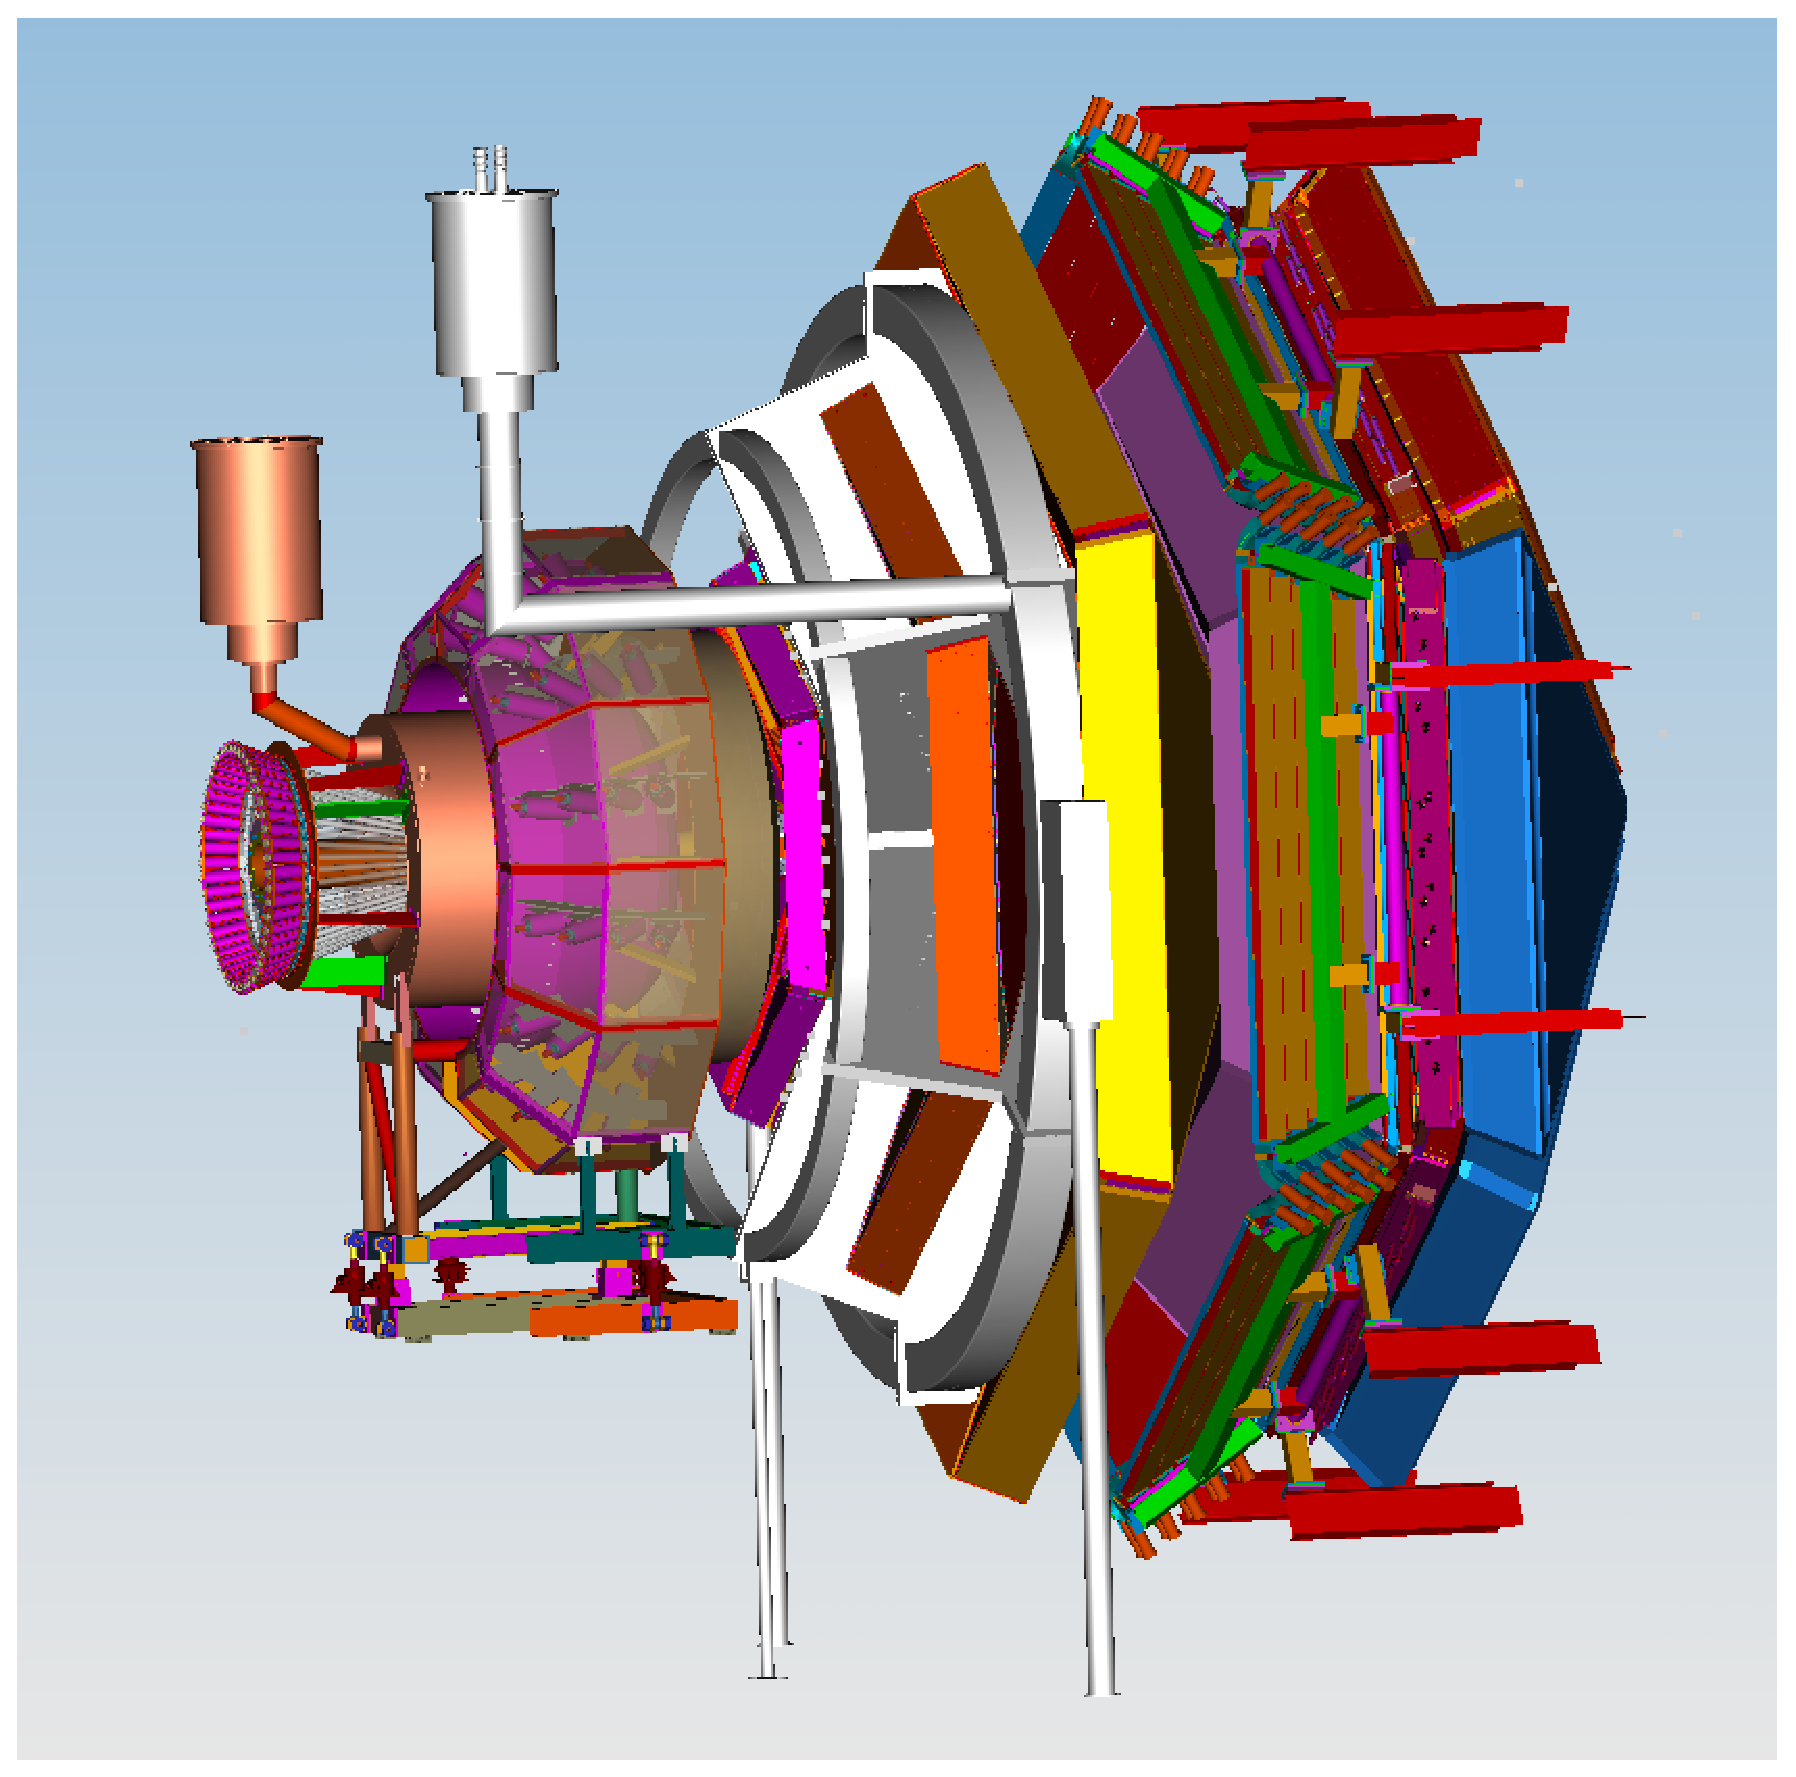
\epsfig{file=Youri/pictures/CD3_CLAS12.eps,width=10.5cm}
\caption{\small{{\tt CLAS12} spectrometer in experimental Hall~B. The
HTCC is shown mounted on the extension of Level-1 of the space frame
just downstream and outside of the solenoid.}}
\label{CLAS12}
\end{center}
\end{figure}
%%%%%%%%%%%%%%%%%%%%%%%%%%%%%%%%%%%%%%%%%%%%%%%%%%%%%%%%%%%%%%%%%%%%%%
   
The HTCC is located between the central and forward detectors of 
{\tt CLAS12}, and is mounted on a separate cart that can be moved along the 
beam direction.  The radiating gas for the HTCC is CO$_2$ at room 
temperature and pressure.  The threshold for the detection of charged 
$\pi$-mesons is 4.9~GeV.  In the entire momentum range below threshold in 
which the detection efficiency for electrons is 99.99\%, the pion rejection 
factor is greater than 300.  For 2.0~GeV pions, it is greater than 750. The 
optical configuration in the HTCC is chosen to be similar to the LTCC 
currently used in {\tt CLAS}.  However, since the detector is positioned 
upstream of the drift chambers and therefore has to be ``thin'', it was 
decided to use one reflection from a single mirror in a given module, as 
opposed to two for the LTCC.  The current design comprises 48 light 
reflection and collection modules.  The main working parameters of the 
HTCC are given in Table~\ref{htcc_parms}.  The overall performance 
requirements and the scope of the primary problems that need to be solved 
are shown in Table~\ref{htcc_reqs}.

%%%%%%%%%%%%%%%%%%%%%%%%%%%%%%%%%%%%%%%%%%%%%%%%%%%%%%%%%%%%%%%%%%%%%%
\begin{table}[htbp]
\begin{center}
\begin{tabular}{|c|c|}  \hline
Channels           & 48 (6 sectors of (2$\times$4) channels each) \\ \hline
Working Gas        & CO$_2$ at 1~atm and room temperature         \\ \hline
Mirror Type        & Ellipsoidal, 48 segments                     \\ \hline
Photomultipliers   & XP4508 (5~in, quartz face-plate)             \\ \hline
Pion Threshold     & 4.9 GeV                                      \\ \hline
Electron Threshold & 15 MeV (electrons)                           \\ \hline
Rejection Factor   & $>$300 at $p<$ 4.9 GeV                       \\ \hline
\end{tabular}
\end{center}
\caption{\small{The main working parameters for the design of the HTCC.}}
\label{htcc_parms}
\end{table}
%%%%%%%%%%%%%%%%%%%%%%%%%%%%%%%%%%%%%%%%%%%%%%%%%%%%%%%%%%%%%%%%%%%%%%

%%%%%%%%%%%%%%%%%%%%%%%%%%%%%%%%%%%%%%%%%%%%%%%%%%%%%%%%%%%%%%%%%%%%%%
\begin{table}[htbp]
\begin{center}
\begin{tabular}{|p{0.4\textwidth}|p{0.55\textwidth}|} \hline
Performance Requirement            & R\&D tasks to be addressed \\ \hline
High electron detection efficiency & Development of technology of ellipsoidal mirror construction. One reflection of {\v C}erenkov photons in most events. \\ \hline 
Run at luminosity $\geq 10^{35}$/cm$^2$s & 48 channels. Flexibility in assigning certain 
angular acceptance to a particular channel. \\ \hline
Acceptance $\Delta \phi = 2\pi$ in angular range $5^\circ \leq \theta \leq 
35^\circ$ & Designing mirrors with no support/alignment parts within the
acceptance.  No dead zones between mirror segments. \\ \hline
Total thickness $\leq$ 200~mg/cm$^2$ & Developing technology of mirror 
construction using components of low density and no residual stress. \\ \hline
Reliability & Safe maintenance and operation of the detector. PMTs and other components can be reached and 
replaced if necessary in-situ. \\ \hline
\end{tabular}
\end{center}
\caption{\small{The overall performance requirements of the HTCC and the
scope of the primary problems that need to be solved.}}
\label{htcc_reqs}
\end{table}
%%%%%%%%%%%%%%%%%%%%%%%%%%%%%%%%%%%%%%%%%%%%%%%%%%%%%%%%%%%%%%%%%%%%%%

\subsection{Optical Requirements}
\label{Optical Requirements}

The upgraded {\tt CLAS12} spectrometer incorporates several major components 
inherited from {\tt CLAS}, such as the Forward Time-of-Flight Counters, 
the Low Threshold {\v C}erenkov Counters, and the Forward Electromagnetic 
Calorimeters.  {\tt CLAS12} will be built in the same experimental area. 
This places constraints on the overall {\tt CLAS12} design, and consequently,
on all detector components, while requiring the most efficient acceptance 
coverage.

The HTCC occupies very limited space downstream of the central detector
and is mounted between the Silicon Vertex Tracker and the Region~1 drift 
chambers.  Fig.~\ref{geometry} illustrates the basic optics of the detector, 
and Fig.~\ref{3dview} shows a 3-dimensional view of the mirror and 
PMTs for one sector.  The design is such that the photons are reflected only 
once by one of the ellipsoidal mirrors and then directly impinge on the 
photocathode of a photomultiplier tube.  However, since the optical design 
must be forgiving in the sense that the light collection efficiency must be 
relatively insensitive to the target length and position, the 5-inch PMTs 
are equipped with {\it Winston} light collection cones to account for the
smearing of the photon distributions due to the influence of the magnetic 
field of the central solenoid on the particle trajectories, 

%%%%%%%%%%%%%%%%%%%%%%%%%%%%%%%%%%%%%%%%%%%%%%%%%%%%%%%%%%%%%%%%%%%%%%
\begin{figure}[ht]
\begin{center}
\epsfig{file=Youri/pictures/CD3_2D_GEO.eps,width=10cm,angle=-90}
\caption{\small{Geometry of the HTCC: an ellipsoidal mirror segment is 
obtained by revolving a corresponding ellipse about its major axis. 
Adjacent segments intersect along planes.  The resulting 4 ellipsoidal 
segments are revolved about the $y$-axis (the beam direction) through 
$\pm$15$^\circ$.  The two highlighted mirror portions are cut to accept 
polar angles from $5^\circ$ to $35^\circ$, and by the median and coil 
planes for one sector, as shown in the right figure.}}
\label{geometry}
\end{center}
\end{figure}
%%%%%%%%%%%%%%%%%%%%%%%%%%%%%%%%%%%%%%%%%%%%%%%%%%%%%%%%%%%%%%%%%%%%%%

%%%%%%%%%%%%%%%%%%%%%%%%%%%%%%%%%%%%%%%%%%%%%%%%%%%%%%%%%%%%%%%%%%%%%%
\begin{figure}
\begin{center}
\epsfig{file=Youri/pictures/CD3_3D_GEO.eps,width=10cm,angle=-90}
\caption{\small{3D-view of the mirror and the PMTs for one HTCC sector.}}
\label{3dview}
\end{center}
\end{figure}
%%%%%%%%%%%%%%%%%%%%%%%%%%%%%%%%%%%%%%%%%%%%%%%%%%%%%%%%%%%%%%%%%%%%%%

The optical properties of the mirrors, Winston cones, and PMTs are 
optimized for maximum reflection and detection of the {\v C}erenkov 
light.  Since much of the {\v C}erenkov light is in the ultraviolet (UV), 
the working surfaces of the mirrors and cones will consist of evaporated
coatings of aluminum, which has a high reflectivity from the near UV 
through the visible wavelength regions.  An evaporated magnesium fluoride 
(MgF$_2$) protective coating will be provided to prevent oxidation of the 
aluminum, while transmitting light through the required wavelength range. 
The photomultiplier tubes will be Photonis XP4508 units with a quartz 
face plate, again, to maximize efficiency in the UV range. 
 
\subsection{Physical Environment} 
\label{Physical Environment}

The HTCC is a single module detector covering all six sectors for scattering 
angles in the range $\theta = 5^\circ$ to $35^\circ$ in the entire 
$\Delta \phi = 2\pi$ range.  Since the detector is a single unit, it can be 
moved along the beam direction or removed from the beam if necessary.  It is 
located in the strong magnetic field of the superconducting solenoid of the 
central detector.  The light collection geometry of the HTCC is such that all 
48 PMTs are located in the fringe field domain at radial distances from
161.3~cm to 194.7~cm from the electron beam.  These distances are chosen to be 
maximal, while still small enough to fit in the Hall~B tunnel and space 
frame infrastructure, while allowing movement of the detector upstream for 
{\tt CLAS12} alignment and maintenance purposes.

The space occupied by the HTCC along the beam direction defines the 
intensity of the {\v C}erenkov photons expected at a given pressure of the 
working gas.  The design of {\tt CLAS12} specifies that the entrance window 
of the {\v C}erenkov counter is located $\sim$0.5~in downstream of the SVT 
of the central detector, and the exit window is 10~cm upstream of the Region~1 
drift chambers.  That leaves the distance that the scattered electrons travel 
in the CO$_2$ radiator of $\sim$131~cm at $\theta = 5^\circ$ and $\sim$181~cm 
at $\theta = 35^\circ$.  The geometry of the HTCC is optimized to keep the
differences in path lengths minimal.  The distribution of magnetic fringe 
fields was taken into consideration in locating the PMTs.  The optics and
estimated signal strength are discussed below.

The intrinsic angular and momentum resolutions of {\tt CLAS12}, along with 
its capability of running at high luminosities, puts serious constraints on 
both the thicknesses and materials that can be used in the HTCC mirror 
construction.  These limitations on materials and estimates of required and 
achievable mirror thicknesses are given in Section~\ref{Mirror}.
 
Another constraint comes from the acceptance specifications for the
Region~1, 2, and 3 (R1, R2, and R3, respectively) drift chambers, which are 
located downstream of the HTCC.  The polar angle acceptance for the drift 
chambers, $\theta = 5^\circ $ to $40^\circ$, is greater than for the HTCC. 
The support structure for the elliptical mirrors has to be located in the 
relatively narrow {\it shadow} region of the coil planes of the {\tt CLAS12} 
torus magnet, and the mirror substrate support built of as light materials 
as possible.
 
\subsection{Overall Design}
\label{Overall design}

The overall approach to working out the HTCC design is a two-fold task,
first to outline the general demands on the HTCC performance and then to 
define the ranges for critical parameters of the major components such 
as the ellipsoidal mirrors.

The main requirements are:

\begin{itemize}
\item High electron detection efficiency, low background;
\item Capability of running at a luminosity of 
$1 \times 10^{35}$~cm$^{-2}$s$^{-1}$;
\item Angular acceptance $5^\circ \leq \theta \leq 35^\circ$ and
$\Delta \phi \approx 2 \pi$;
\item Lightweight -- as little material as possible within the acceptance to 
meet the expected angular and momentum resolutions of {\tt CLAS12} ($\delta 
\theta \leq 1.5$~mrad, $\delta \phi \leq 5$~mrad, and $\Delta p/p \leq 1\%$).
\end{itemize}

%%%%%%%%%%%%%%%%%%%%%%%%%%%%%%%%%%%%%%%%%%%%%%%%%%%%%%%%%%%%%%%%%%%%%%
\begin{figure}
\begin{center}
\epsfig{file=Youri/pictures/CD3_FIG2_3_1.eps,width=7cm,angle=-90}
\caption{\small{A view of the front face of the HTCC showing the 
entrance window in red.}}
\label{back}
\end{center}
\end{figure} 
%%%%%%%%%%%%%%%%%%%%%%%%%%%%%%%%%%%%%%%%%%%%%%%%%%%%%%%%%%%%%%%%%%%%%%

A front view of the HTCC is shown in Fig.~\ref{back}.  Some specific 
features of the HTCC design include:

\begin{itemize}
\item Thin entry and exit windows of black Kapton or Tedlar film\\ 
($\sim$3.5~mg/cm$^2$ and $\sim$11~mg/cm$^2$, respectively);
\item Ultra-thin, self-supporting mirror structure;
\item Capability of working with different types of Tungsten M{\o}ller 
shields. 
\end{itemize}

The total radiation length of the detector is $\sim$1.7\%, including 
contributions of the CO$_2$ radiator gas ($\sim$0.9\%), and of the mirror 
($<0.8$\%). Since the number of photons per event is proportional to the 
total radiation length of the radiator, the only way to decrease the 
thickness of the detector without compromising its performance is to use 
thinner mirror backing.  Figs.~\ref{resolution}a, b, and c illustrate the 
changes in the {\tt CLAS12} resolution for different mirror thicknesses: 
standard ($\sim$200~mg/cm$^2$) and reduced to $\sim$100~mg/cm$^2$.  The 
results show relatively small improvements in momentum, angular, and spatial 
resolutions for thinner mirrors, indicating that the influence of the mirror 
thickness is small or comparable with contributions of other {\tt CLAS12} 
detector components.

%%%%%%%%%%%%%%%%%%%%%%%%%%%%%%%%%%%%%%%%%%%%%%%%%%%%%%%%%%%%%%%%%%%%%%
\begin{figure}
\begin{center}
\epsfig{file=Youri/pictures/FIG2_3_2a.eps,width=6.5cm,angle=-90}
\vspace{0.5in}
\epsfig{file=Youri/pictures/FIG2_3_2b.eps,width=6.5cm,angle=-90}
\vspace{0.5in}
\epsfig{file=Youri/pictures/FIG2_3_2c.eps,width=6.5cm,angle=-90}
\vspace{0.5in}
\caption{\small{Momentum, angular, and spatial resolution of {\tt CLAS12} 
for pions.}}
\label{resolution}
\end{center}
\end{figure} 
%%%%%%%%%%%%%%%%%%%%%%%%%%%%%%%%%%%%%%%%%%%%%%%%%%%%%%%%%%%%%%%%%%%%%%

\section{Optical Design and Construction}
\label{Details}

The most challenging aspect of the HTCC is the construction of the
elliptical mirrors.  In addition to being very lightweight and 
self-supporting, there must not be shadowing among adjacent mirrors or gaps 
between them. This problem has been worked out as follows: each mirror 
surface is an ellipsoid of rotation, so the line of intersection of adjacent  
mirror surfaces is curved.  Two coplanar ellipses, each revolved about its 
major axis, give two ellipsoids of rotation, (1) and (2), represented by the
following equations:
 
\begin{eqnarray}
\label{elips}
\frac{x^2+(y-y_1)^2}{a_1^2} &+& \frac{(z-z_1)^2}{b_1^2} = 1  \nonumber\\
\hspace{1in}\\
\frac{x^2+(y \cdot \cos \theta-z \cdot \sin \theta)^2}{a_2^2} &+& 
\frac{(y \cdot \sin \theta-z \cdot \cos \theta)^2}{b_2^2} = 1. \nonumber  
\end{eqnarray}

\noindent
In the above, $(0,y_1,z_1)$ are the coordinates of the center of the ellipse 
(1), $a_1, a_2$, and $b_1, b_2$, respectively, are the minor and major radii 
of the ellipses, and $\theta$ is the angle between the major axis $b_2$ and 
the $z$-axis in the $y-z$-plane.  Considering the system in the $x = c < a_1$  
plane, we get (assuming $a_1 < a_2$): 

\begin{eqnarray}
\label{elips_var}
\frac{(y-y_1)^2}{a_1^2} &+& \frac{(z-z_1)^2}{b_1^2} = c_1^2 \nonumber \\
\hspace{1in}\\
\frac{(y \cdot \cos \theta-z \cdot \sin \theta)^2}{a_2^2} &+& 
\frac{(y \cdot \sin \theta-z \cdot \cos \theta)^2}{b_2^2} = c_2^2. \nonumber  
\end{eqnarray} 
 
By excluding one variable from eq.(\ref{elips_var}), we arrive at a general 
quartic equation:

\begin{equation}
p_0z^4 + p_1 z^3 + p_2 z^2 + p_1 z + p_4=0, \nonumber \\
\end{equation} 

\noindent
which always can be solved, and in the case of the HTCC geometry, has 
two roots (see Fig.~\ref{figelips}). So, from eq.(\ref{elips_var}),  
we obtain two roots $P_1^{(c)}(y_1,z_1)$ and $P_2^{(c)}(y_2,z_2)$ 
in the plane $x = c$; they also satisfy eq.(\ref{elips}) at $x = c$: 
$P_1^{(c)}(c,y_1,z_1)$ and $P_2^{(c)}(c,y_2,z_2)$ are the roots of 
eq.(\ref{elips}).  Two other roots of eq.(\ref{elips}) can be found at 
$x=0$ (the $y-z$-plane): $P_3(0,y_1,z_1)$ and $P_4(0,y_2,z_2)$.  Three out 
of any four roots define a plane.  It can be shown that the remaining 
root belongs to the same plane as well.  Since we arbitrarily used $x = c$,  
all points of intersection (intersection curve) of the two ellipsoids belong
to the same plane.  This allows us to build mutually self-supporting
ellipsoidal mirrors in which there are no gaps or shadowing of one mirror by 
the next.  As a result, the cutting of the segments along the perimeter and
the final assembly become relatively simple. Moreover, there will be no 
shadowing of one mirror by another, and no ``dead'' zones for any electrons 
from the target within the acceptance.  This also eliminates the need of 
having a support structure for any single mirror segment, and consequently 
makes it possible to construct the most efficient and lightweight mirror. 

%%%%%%%%%%%%%%%%%%%%%%%%%%%%%%%%%%%%%%%%%%%%%%%%%%%%%%%%%%%%%%%%%%%%%%
\begin{figure}
\begin{center}
\epsfig{file=Youri/pictures/CD_2_FIG2_4_1.eps,width=10cm,angle=-90}
\caption{\small{Ellipses of adjacent mirrors intersecting in two points.}}
\label{figelips}
\end{center}
\end{figure} 
\begin{figure}
\begin{center}
\epsfig{file=Youri/pictures/CD3_PLANES.eps,width=10cm,angle=-90}
\caption{\small{Planes of intersection of adjacent mirror segments.}}
\label{planes}
\end{center}
\end{figure} 
%%%%%%%%%%%%%%%%%%%%%%%%%%%%%%%%%%%%%%%%%%%%%%%%%%%%%%%%%%%%%%%%%%%%%%

Fig.~\ref{planes} shows four intersecting mirrors forming half of the mirror  
array for one sector.  The coordinates of the points defining the planes of 
intersection between segments were used in the corresponding Monte Carlo 
simulations.  Fig.~\ref{mirror} illustrates the concept of the compound 
elliptical mirror assembly.  The approximate dimensions of segment \#4 
are given in inches.

%%%%%%%%%%%%%%%%%%%%%%%%%%%%%%%%%%%%%%%%%%%%%%%%%%%%%%%%%%%%%%%%%%%%%%
\begin{figure}
\begin{center}
\epsfig{file=Youri/pictures/CD3_SEGM_CUT.eps,width=8cm,angle=-90}
\caption{\small{Elliptical mirror segments cut along the planes of 
intersection.  A set of four segments cover half of the acceptance of one 
sector.  An identical set covers the other half of the acceptance.}}
\label{mirror}
\end{center}
\end{figure} 
%%%%%%%%%%%%%%%%%%%%%%%%%%%%%%%%%%%%%%%%%%%%%%%%%%%%%%%%%%%%%%%%%%%%%%

The tolerances for construction are critical for HTCC performance. 
The typical tolerances for cutting the substrates are of order 0.001~in 
and have been achieved in prototyping.  So, the expected average
deviation from the nominal geometry would be mostly due to the accuracy that 
can be achieved at the assembly stage.  It is anticipated to keep the assembly 
tolerance within $\pm$0.010~in for one mirror segment.  Parallel shifts 
will not affect the light collection because of the large overall acceptance,
whereas unwanted rotation of a segment during assembly might require some 
adjustment of the PMT positions, which would be unacceptable.  At the given 
average half width of the segments, $\sim$5~in (see Fig.~\ref{mirror}), the
angular equivalent of $\pm$0.01~in is $\sim$2~mrad or less.  This is the 
worst possible case since all segments except \#1 are of length greater than 
5.60~in.  The average distance between the mirrors and the corresponding PMTs 
is $\sim$80.5~in. Therefore, the shift of the image in the focal plane of 
the PMTs is less then 0.15~in ($\sim$3.8~mm). This estimate will be
examined in R\&D. 

\subsection{Mirror Prototyping}
\label{Mirror}
 
All of the main features of the HTCC and the properties of its components 
will be examined and checked by prototyping and testing of the key elements. 
In this section we present results on the prototyping of one mirror segment 
obtained in FY06, and describe current R\&D efforts on building a mirror 
consisting of 3 mirror segments.  The main R\&D goal is to find ways of 
building an elliptical mirror of:

\begin{itemize}
\item 200 mg/cm$^2$ total thickness;
\item minimal residual stress (no adjustment in-situ);
\item highest possible specular reflectivity of working surface;
\item reasonable cost.
\end{itemize}

A mirror substrate consists of a thermally shaped plain Mylar film of 
thickness 0.005~in, laminated to an ellipsoidal substrate made of rigid 
Polymethacrylimide polymer foam Rohacell HF31 ($\rho \approx 31$~mg/cm$^3$). 
In the entire construction procedure, the working surface of the Mylar film 
stays untouched. The aluminum reflector and optical coating of magnesium 
fluoride (MgF$_2$) will be vacuum deposited onto the mylar surface after 
the substrate and mylar are joined as a completed unit. A set of molding 
tools is used for the shaping of the Mylar film into the ellipsoidal shape 
that mates precisely with the Rohacell substrate to avoid residual stresses.  
One of the mold fixtures attached to the bottom-plate of the vacuum chamber 
is shown in Fig.~\ref{mold}.  The top surface of the mold is cut to the 
precise shape of the specified ellipsoid of rotation by computer-controlled 
milling using a ball-end mill. The thickness of the film is taken into 
account.  The top of the mold is then polished to remove scalloping left 
after milling.  The Mylar film is shaped by this surface, so the finish 
has to be smooth enough to avoid a {\it'' telegraph wire''} effect, although 
the surface does not have to be of mirror quality.  
 
%%%%%%%%%%%%%%%%%%%%%%%%%%%%%%%%%%%%%%%%%%%%%%%%%%%%%%%%%%%%%%%%%%%%%%
\begin{figure}
\begin{center}
\epsfig{file=Youri/pictures/CD_2_MOLD.eps,width=10cm,angle=-90}
\caption{\small{The mold installed on the bottom-plate.}}
\label{mold}
\end{center}
\end{figure} 
%%%%%%%%%%%%%%%%%%%%%%%%%%%%%%%%%%%%%%%%%%%%%%%%%%%%%%%%%%%%%%%%%%%%%%

For better control of the Mylar film edges and to minimize effects of 
thermal contraction, a thin aluminum support guard is installed surrounding 
the mold, as shown in Fig.~\ref{support1}.  There is a small gap of 1/8-in 
width left between the support and mold.  The support has a profile (shown 
in red) parallel to the edge of the ellipsoidal surface of the mold.  The gap 
is so small that the edge of the shaped Mylar film is defined not by the
mold, but by the support.  This results in a better alignment of the film 
with the foam substrate while gluing.

%%%%%%%%%%%%%%%%%%%%%%%%%%%%%%%%%%%%%%%%%%%%%%%%%%%%%%%%%%%%%%%%%%%%%%
\begin{figure}
\begin{center}
\epsfig{file=Youri/pictures/CD_2_SUPPORT.eps,width=10cm,angle=-90}
\caption{\small{The support installed around the mold.}}
\label{support1}
\end{center}
\end{figure}  
%%%%%%%%%%%%%%%%%%%%%%%%%%%%%%%%%%%%%%%%%%%%%%%%%%%%%%%%%%%%%%%%%%%%%%

In Fig.~\ref{vacuum} the wall of the vacuum chamber (molding box) attached 
to the bottom plate is shown.  There are high-temperature-rated vacuum 
o-rings installed both on the top and bottom of the wall.
 
%%%%%%%%%%%%%%%%%%%%%%%%%%%%%%%%%%%%%%%%%%%%%%%%%%%%%%%%%%%%%%%%%%%%%%
\begin{figure}
\begin{center}
\epsfig{file=Youri/pictures/CD_2_WALL.eps,width=7cm,angle=-90}
\caption{\small{The vacuum chamber with the mold.}}
\label{vacuum}
\end{center}
\end{figure}  
%%%%%%%%%%%%%%%%%%%%%%%%%%%%%%%%%%%%%%%%%%%%%%%%%%%%%%%%%%%%%%%%%%%%%%

The profile of the top of the wall is cylindrical, such that there is an 
approximately constant clearance of $\sim$1/4~in between this surface and 
the ellipsoidal surface of the mold.  The inside gap between the wall and 
support is quite wide.  It has to be wide enough for the Mylar film to 
form concave channels under applied pressure.  These channels are formed all 
the way around the support and are necessary for tension relief when the  
chamber is being cooled down and then depressurized.

%%%%%%%%%%%%%%%%%%%%%%%%%%%%%%%%%%%%%%%%%%%%%%%%%%%%%%%%%%%%%%%%%%%%%%
\begin{figure}
\begin{center}
\epsfig{file=Youri/pictures/CD_2_MYLAR.eps,width=10cm,angle=-90}
\caption{\small{The vacuum chamber with the mold and the pre-cut Mylar film.}}
\label{Mylar}
\end{center}
\end{figure} 
%%%%%%%%%%%%%%%%%%%%%%%%%%%%%%%%%%%%%%%%%%%%%%%%%%%%%%%%%%%%%%%%%%%%%%

A portion of Mylar film is placed on top of the vacuum chamber, as shown 
(in transparent yellow) in Fig.~\ref{Mylar}. The top surface of the 
Mylar remains untouched during cutting and installation of the film. 
A flange is placed on the top of the Mylar and tightened down to the wall.
Then the air in the chamber is pumped out so that the Mylar is 
deflected under atmospheric pressure, as in Fig.~\ref{Mylar_var}.

%%%%%%%%%%%%%%%%%%%%%%%%%%%%%%%%%%%%%%%%%%%%%%%%%%%%%%%%%%%%%%%%%%%%%%
\begin{figure}
\begin{center}
\epsfig{file=Youri/pictures/CD_2_FLANGE.eps,width=10cm,angle=-90}
\caption{\small{The vacuum chamber with the mold and the Mylar film.}}
\label{Mylar_var}
\end{center}
\end{figure} 
%%%%%%%%%%%%%%%%%%%%%%%%%%%%%%%%%%%%%%%%%%%%%%%%%%%%%%%%%%%%%%%%%%%%%%

At this point, while still at room temperature, the Mylar is touching 
the mold, and the area of contact between them is about 60-70\% of maximum. 
To provide a 100\% contact, the vacuum chamber is heated in an oven to
a temperature of 170$^\circ$C. During the heating process, which takes about 
4~hours, the chamber remains connected to a vacuum pump located outside the 
oven.  To increase the deflection of the unsupported portion of Mylar film 
(along the wall), additional pressure is applied to the film.  This is done 
by covering the vacuum chamber with a lid installed on the top of the flange, 
as shown in Fig.~\ref{Mylar_pres}.  The volume under the lid is then 
pressurized with dry nitrogen.

%%%%%%%%%%%%%%%%%%%%%%%%%%%%%%%%%%%%%%%%%%%%%%%%%%%%%%%%%%%%%%%%%%%%%%
\begin{figure}
\begin{center}
\epsfig{file=Youri/pictures/CD_2_LID.eps,width=7cm,angle=-90}
\caption{\small{Vacuum chamber equipped with lid allowing molding of Mylar 
film at higher pressures.}}
\label{Mylar_pres}
\end{center}
\end{figure} 
%%%%%%%%%%%%%%%%%%%%%%%%%%%%%%%%%%%%%%%%%%%%%%%%%%%%%%%%%%%%%%%%%%%%%%

The maximal differential pressure applied to the Mylar can be as high 
as 3~kg/cm$^2$.  Tested stable results were obtained at differential 
pressures in the range from 2.0 to 2.55~kg/cm$^2$, depending on the
temperature.  The cooling of the chamber back to room temperature is the 
last step in the thermal shaping.  The working differential pressure, once 
reached, is monitored and kept constant during the entire cooling cycle. 
After completion, the differential pressure is brought back to atmosphere 
and the lid is removed.  A frame, shown in Fig.~\ref{glue}, is glued onto 
the already shaped Mylar film. The bottom surface of the frame has the 
required ellipsoidal shape.  On the top there is a groove cut for a vacuum 
o-ring.  In the figure, several installed studs are shown in red. 
Fig.~\ref{glue_var} illustrates the gluing of the frame onto the pressurized 
thermally shaped Mylar.  The largest portion of the Mylar, even while 
pressurized, is stress free.  That portion of the surface that is in full 
contact with the mold, is leaning on it, and therefore no stresses are 
involved here. Only the unsupported deflected portion of Mylar that is out 
of the gluing frame is under stress.  After the glue is polymerized, a flat 
Plexiglas lid is attached to the frame, and the vacuum chamber is released. 
The deflected portion of Mylar provides stress relief.  The Mylar film, 
shaped at no residual stress, together with the frame and lid, is cut out as a 
single unit for future use. 

%%%%%%%%%%%%%%%%%%%%%%%%%%%%%%%%%%%%%%%%%%%%%%%%%%%%%%%%%%%%%%%%%%%%%%
\begin{figure}
\begin{center}
\epsfig{file=Youri/pictures/CD_2_FRAME.eps,width=10cm,angle=-90}
\caption{\small{The HTCC gluing frame.}}
\label{glue}
\end{center}
\end{figure} 
%%%%%%%%%%%%%%%%%%%%%%%%%%%%%%%%%%%%%%%%%%%%%%%%%%%%%%%%%%%%%%%%%%%%%%

%%%%%%%%%%%%%%%%%%%%%%%%%%%%%%%%%%%%%%%%%%%%%%%%%%%%%%%%%%%%%%%%%%%%%%
\begin{figure}
\begin{center}
\epsfig{file=Youri/pictures/CD_2_FRAME_LID.eps,width=10cm,angle=-90}
\caption{\small{Gluing frame with Plexiglas lid on the top and Mylar 
attached to the bottom.}}
\label{glufr}
\end{center}
\end{figure}
%%%%%%%%%%%%%%%%%%%%%%%%%%%%%%%%%%%%%%%%%%%%%%%%%%%%%%%%%%%%%%%%%%%%%%

%%%%%%%%%%%%%%%%%%%%%%%%%%%%%%%%%%%%%%%%%%%%%%%%%%%%%%%%%%%%%%%%%%%%%%
\begin{figure}
\begin{center}
\epsfig{file=Youri/pictures/CD_2_FRAME_GLUED.eps,width=10cm,angle=-90}
\caption{\small{The frame glued onto the thermally shaped Mylar film leaves 
the film stress free after the chamber is depressurized.}}
\label{glue_var}
\end{center} 
\end{figure}
%%%%%%%%%%%%%%%%%%%%%%%%%%%%%%%%%%%%%%%%%%%%%%%%%%%%%%%%%%%%%%%%%%%%%%

The other important component of the mirror is the mechanical support
substrate, which is made of rigid foam.  A sheet of polymer foam is sanded 
down, under its own weight, until it provides a flat base.  The top of the 
flat sheet is cut by CNC milling to the concave ellipsoidal shape, which 
mates to the back surface of the Mylar mirror substrate, as seen in 
Fig.~\ref{flatface}.  The length and width are appropriate for gluing the 
frame and mold.

%%%%%%%%%%%%%%%%%%%%%%%%%%%%%%%%%%%%%%%%%%%%%%%%%%%%%%%%%%%%%%%%%%%%%%
\begin{figure}
\begin{center}
\epsfig{file=Youri/pictures/FIG2_5_9.eps,width=10cm,angle=-90}
\caption{\small{The substrate: flat face down, cylindrical top.}}
\label{flatface}
\end{center} 
\end{figure}
%%%%%%%%%%%%%%%%%%%%%%%%%%%%%%%%%%%%%%%%%%%%%%%%%%%%%%%%%%%%%%%%%%%%%%

In order to process the front (working) surface, the substrate is mounted 
on an auxiliary table and glued to it along the edges at several locations, 
as shown in Fig.~\ref{auxiliar}.  The top of the table and back of the 
substrate have precisely the same ellipsoidal shape, thus providing the 
required rigidity for further processing.

%%%%%%%%%%%%%%%%%%%%%%%%%%%%%%%%%%%%%%%%%%%%%%%%%%%%%%%%%%%%%%%%%%%%%%
\begin{figure}
\begin{center}
\epsfig{file=Youri/pictures/FIG2_5_10.eps,width=8cm,angle=-90}
\caption{\small{The substrate mounted on the auxiliary table.}}
\label{auxiliar}
\end{center} 
\end{figure}
%%%%%%%%%%%%%%%%%%%%%%%%%%%%%%%%%%%%%%%%%%%%%%%%%%%%%%%%%%%%%%%%%%%%%%

Fig.~\ref{computer} shows the cutting of the working surface to the shape 
of an ellipsoid.  The ellipsoid parameters were defined by taking into
account the thickness of the anticipated glue joint and of the thermally 
shaped Mylar film.  The process was optimized to achieve a surface finish 
on the foam smooth enough so that no polishing would be necessary. Due to 
the properties of foam structure, there were no scallops observed after 
milling.  In Fig.~\ref{prototype} sample pieces of the thermally shaped 
Mylar films are shown, along with the mold used in shaping them, and the 
completely processed foam substrate mounted on the auxiliary table.

%%%%%%%%%%%%%%%%%%%%%%%%%%%%%%%%%%%%%%%%%%%%%%%%%%%%%%%%%%%%%%%%%%%%%%
\begin{figure}
\begin{center}
\epsfig{file=Youri/pictures/FIG2_5_11.eps,width=10cm,angle=-90}
\caption{\small{Computer-controlled cutting of the ellipsoidal surface of 
the foam substrate.}}
\label{computer}
\end{center} 
\end{figure}
%%%%%%%%%%%%%%%%%%%%%%%%%%%%%%%%%%%%%%%%%%%%%%%%%%%%%%%%%%%%%%%%%%%%%%

%%%%%%%%%%%%%%%%%%%%%%%%%%%%%%%%%%%%%%%%%%%%%%%%%%%%%%%%%%%%%%%%%%%%%%
\begin{figure}
\begin{center}
\epsfig{file=Youri/pictures/CD3_GLUING.eps,width=10cm,angle=-90}
\caption{\small{Precision assembly of the mirror substrate.}}
\label{prototype}
\end{center}
\end{figure}
%%%%%%%%%%%%%%%%%%%%%%%%%%%%%%%%%%%%%%%%%%%%%%%%%%%%%%%%%%%%%%%%%%%%%%

The final step in mirror construction is the gluing of the shaped Mylar 
onto the ellipsoidal substrate.  The gluing frame, with transparent 
Plexiglas lid on the top and the Mylar film attached to the bottom (see 
Fig.~\ref{glufr}), is pressurized at a differential pressure up to 
$\sim$2$\times$10$^{-2}$~Torr, so that the film bulges out beyond its 
normal convexity.  Low viscosity de-gassed epoxy with extended 
polymerization time is uniformly applied to the ellipsoidal surface of 
the substrate that remains attached to the auxiliary table.  Then the 
pressurized frame with bulged Mylar is placed on top of the substrate 
slowly enough to let trapped air bubbles escape. A transparent lid allows 
visual control of the quality of the joint.  The Mylar is fully pressed 
against the substrate, and stays under uniformly distributed pressure 
until the epoxy is cured.  The position of the frame relative to the table 
is controlled by using special tooling for precision assembly of the mirrors.  
After curing, the frame is depressurized, the lid removed, and the auxiliary 
table with its components is placed back on the CNC milling machine.  The 
inner portion of the composite substrate is directly cut out through an 
opening on the frame.  Measurements have shown that the total thickness of 
the composite substrate was 73-74~mg/cm$^2$.  There is a potential of 
further decreasing a mirror's thickness without altering the technology 
described in this section.  It would leave some contingency in varying the 
mirror thickness within a factor of $\sim$2, while optimizing the overall 
rigidity.

In 2007-2008 R\&D is planned to check the last step of construction of the
mirror consisting of three different ellipsoidal segments.  A critical 
issue to be addressed is whether the estimated tolerances of assembly can 
be achieved. 

Each of the three mirror segments, once built according to already 
established technology, is put on the modified auxiliary table with special 
trim grooves for compound-angle cuts. Then all four sides (one at a time) 
are cut on a 5-axis milling machine at appropriate angles (all different), 
defining the orientation of the planes along which the ellipsoids intersect.  
The accuracy of cutting (including positioning) is typically $\pm$0.001~in 
or better. Fig.~\ref{compl_cut} shows a substrate that has been processed 
along all sides (in yellow) mounted on the modified auxiliary table.

%%%%%%%%%%%%%%%%%%%%%%%%%%%%%%%%%%%%%%%%%%%%%%%%%%%%%%%%%%%%%%%%%%%%%%
\begin{figure}
\begin{center}
\epsfig{file=Youri/pictures/CD_2_SBS_ON_TBL.eps,width=10cm,angle=-90}
\caption{\small{Completely cut substrate mounted on the modified auxiliary 
table.}}
\label{compl_cut}
\end{center}
\end{figure}
%%%%%%%%%%%%%%%%%%%%%%%%%%%%%%%%%%%%%%%%%%%%%%%%%%%%%%%%%%%%%%%%%%%%%%

The sides of all segments are trimmed using their own tables since the 
angles and dimensions are different for each. But, the back surfaces of 
all three segments, and the top of the corresponding tables, are cylindrical 
with the same parameters. So, the segments can be mounted next to each 
other on a larger table with the top surface of the same cylindrical shape. 
This is illustrated in Fig.~\ref{segments}.  After alignment checks of 
the substrates, they will be glued together along the planes of intersection.

%%%%%%%%%%%%%%%%%%%%%%%%%%%%%%%%%%%%%%%%%%%%%%%%%%%%%%%%%%%%%%%%%%%%%%
\begin{figure}
\begin{center}
\epsfig{file=Youri/pictures/CD_2_B_TBL_SBS.eps,width=10cm,angle=-90}
\caption{\small{Mirror segments mounted on the Big Table.  The left and 
right sides of the mirrors are planes along which will be glued adjacent 
combined mirrors.}}
\label{segments}
\end{center}
\end{figure}
%%%%%%%%%%%%%%%%%%%%%%%%%%%%%%%%%%%%%%%%%%%%%%%%%%%%%%%%%%%%%%%%%%%%%%

\subsection{Light Collection Cones}
\label{Light Collection}

GEANT simulations of the HTCC optics and performance show that for a
point-like target with no magnetic field, almost all {\v C}erenkov photons 
from each segment are focused on its corresponding PMT photocathode of 
diameter 110~mm. This is minimal for the Photonis 5-in PMTs.  In experiments 
with {\tt CLAS12}, standard cryogenic targets are 50-mm long, and in some 
experiments, targets as long as 100~mm can be used.  For all experiments 
with electron beams, the superconducting solenoid and the {\v C}erenkov 
counters will be used.  As was mentioned in 
Section~\ref{Optical Requirements}, to have efficient {\v C}erenkov light 
collection for extended targets in magnetic fields, light collection (Winston) 
cones are necessary.  To define the main parameters for the Winston Cones, we 
required an opening diameter of 7.5~in and a distance from the PMT 
photocathode to be equal to 8~in, allowing magnetic shields to be extended far 
enough beyond the photocathode.  Direct comparison of the angular acceptance 
of the Winston Cones with results from Monte Carlo simulations, showed that 
the Winston Cone's acceptance is much wider, and the opening diameter is big 
enough to collect at least 95\% of the {\v C}erenkov light in experiments 
with both polarities of the {\tt CLAS12} torus magnet without any 
adjustments of the PMT locations or orientations.

There are well established and experimentally checked technologies for 
constructing Winston Cones.  Such light concentrators were built for the 
existing Low Threshold {\v C}erenkov Counter (LTCC) of {\tt CLAS} by 
electro-forming technology and have shown sustained undiminished 
performance for more than a decade.  The technical specifications and 
requirements of the proposed Winston cone for the HTCC, similar to those 
used in {\tt CLAS}, are given in Table~\ref{HTCCtab}.  The corresponding 
parameters are given in Fig.~\ref{Winston}.

%%%%%%%%%%%%%%%%%%%%%%%%%%%%%%%%%%%%%%%%%%%%%%%%%%%%%%%%%%%%%%%%%%%%%%
\begin{figure}
\begin{center}
\epsfig{file=Youri/pictures/CD3_WC.eps,width=10cm,angle=-90}
\caption{\small{Winston cones for the HTCC.}}
\label{Winston}
\end{center}
\end{figure}
%%%%%%%%%%%%%%%%%%%%%%%%%%%%%%%%%%%%%%%%%%%%%%%%%%%%%%%%%%%%%%%%%%%%%%

%%%%%%%%%%%%%%%%%%%%%%%%%%%%%%%%%%%%%%%%%%%%%%%%%%%%%%%%%%%%%%%%%%%%%%
\begin{table}
\begin{center}
\begin{tabular}{|l|c|c|} \hline
Specification             & Date              & Source    \\ \hline
Winston Cone Definition   &                   &           \\ \hline
\begin{minipage}[l]{0.68\textwidth} A Winston Cone is a non-imaging 
light collector designed to collect light from a range of incident 
angles on a given circular area and to collect that light onto a 
smaller area.  The Winston Cone is not a focusing device, but it is 
highly efficient in collecting light.  In general, the shape is 
that of a parabola that revolves about the axis of symmetry of the 
parabola.\end{minipage}   &                   &           \\ \hline
Basics                    &                   &           \\ \hline
\begin{minipage}[l]{0.68\textwidth}
Material = nickel alloy outer surface with inner coatings of aluminum and magnesium fluoride (see below)
\end{minipage}            & 12/2006           & P. Stoler \\ \hline
Weight = $\sim$4 lbs      & 12/2006           & Y. Sharabian \\ \hline
Life time = 30 years with no optical degradation & 12/2006  & P. Stoler\\ \hline
Dimensions  = 7.5 in $\times$ 8.0 in long     & 12/2006 & Y. Sharabian\\ \hline
\begin{minipage}[l]{0.68\textwidth}
Optical and structural properties tolerant to a high radiation dose 
of 20 Mrad/20 years
\end{minipage}            & 09/1991           & C. Zorn    \\ \hline
Most radiation consists of x-rays with some relativistic particles & 05/1992 & C. Zorn\\ \hline
Manufacturing = electroforming          &                   &            \\ \hline
Slope errors $<1^\circ$   & 12/2006           & D. Kashy   \\ \hline
Surface finish of Root Mean Square = 0.5 $\mu$m & 12/2006 & Y. Sharabian\\ \hline
\begin{minipage}[c]{0.68\textwidth}
Scratches occurring in forming operation, etc. need not be removed 
provided in the final product there are less than 4/cone and\\ 
\begin{tabular}{cl}
1) & they are less than 2.54~cm in length \\
2) & they are less than 0.15~$\mu$m deep \\
\end{tabular} \\
Open ends flat within 0.03~in
\end{minipage}            & 12/2006           & Y. Sharabian \\ \hline
Optics                    & 12/2006           & Y. Sharabian \\ \hline
\begin{minipage}[c]{0.68\textwidth}
\begin{tabular}{cl}
 & Acceptance angle for incident light = 28.3$^\circ$ \\
 & Reflectivity $>$88\% between 220~nm and 600~nm \\
 & for all glancing angles $<$30$^\circ$ \\
\end{tabular} \\
\end{minipage}             &                  &              \\ \hline
\end{tabular}
\end{center}
\caption{\small{Specifications for the HTCC Winston cones for {\tt CLAS12}.}} 
\label{HTCCtab}
\vspace{0.5cm}
\end{table}
%%%%%%%%%%%%%%%%%%%%%%%%%%%%%%%%%%%%%%%%%%%%%%%%%%%%%%%%%%%%%%%%%%%%%%

%%%%%%%%%%%%%%%%%%%%%%%%%%%%%%%%%%%%%%%%%%%%%%%%%%%%%%%%%%%%%%%%%%%%%%
\begin{table}
\begin{center}
\begin{tabular}{|c|c|c|} \hline
{\bf MATERIAL} & 12/2006 & P. Stoler \\ \hline
\begin{minipage}[c]{0.68\textwidth}
Nickel Alloy: \\
\begin{tabular}{cl}
 &   Thickness = 0.040-in nominal \\
 &   Application method = electro-formed \\
\end{tabular} \\     
Aluminum: \\
\begin{tabular}{cl}
 &   Thickness $\approx$ 0.04~$\mu$m \\
 &   Application method = vacuum (vapor) deposition \\
 &   Non-magnetic \\
\end{tabular} \\ 
Magnesium fluoride (protective coating) \\ 
\begin{tabular}{cl}
 &   Thickness = as required to meet reflectivity specifications \\ 
 &   Application method = vacuum (vapor) deposition \\
 &   Non-magnetic \\
\end{tabular} 
\end{minipage} & & \\ \hline \hline
\begin{minipage}[l]{0.68\textwidth}
{\bf ENVIRONMENTAL} 
\end{minipage} & 12/2006 & Y. Sharabian \\ \hline
\begin{minipage}[l]{0.68\textwidth}
Operating in CO$_2$ at 1.001~atm, temperature = 22$^\circ$C;
Stored in plastic bag w/ambient air to avoid dust contamination;
DO NOT contact reflective surface with anything;
Wash reflective surface w/only optical liquid.
\end{minipage} & & \\ \hline
\end{tabular}
\end{center}
\caption{\small{Specifications for the HTCC Winston cones for {\tt CLAS12}.}}
\label{TCC}
\end{table}
%%%%%%%%%%%%%%%%%%%%%%%%%%%%%%%%%%%%%%%%%%%%%%%%%%%%%%%%%%%%%%%%%%%%%%

\section{DAQ for HTCC}

Signals from the {\v C}erenkov counter will be used in generation of 
the {\tt CLAS12} event trigger and for timing purposes.  The PMTs will 
supply an anode signal over a coaxial cable to a passive splitter installed 
on the forward carriage.  One of the output signals from the splitter will go 
to a flash ADC (see Fig.~\ref{singlHTCC}) and the other one to will go
to a timing discriminator connected to a pipeline TDC. 
 
%%%%%%%%%%%%%%%%%%%%%%%%%%%%%%%%%%%%%%%%%%%%%%%%%%%%%%%%%%%%%%%%%%%%%%
\begin{figure}
\vspace{2.0cm}
\begin{center}
\epsfig{file=Youri/pictures/CD_2_SERJ.eps,width=5.5cm,angle=-90}
\caption{\small{Single channel scheme of readout for the HTCC.}}
\label{singlHTCC}
\end{center}
\end{figure}
%%%%%%%%%%%%%%%%%%%%%%%%%%%%%%%%%%%%%%%%%%%%%%%%%%%%%%%%%%%%%%%%%%%%%%

The flash ADC will have 12-bit resolution and a 250~MHz clock. The pipeline 
TDCs will provide 85~ps time resolution.  The timing discriminators will 
have built-in scalers for each channel.  The sums from the flash ADCs will 
be delivered to the trigger processing boards and will be used to generate 
the Level-1 trigger, along with the other fast detectors of {\tt CLAS12}. 
The mirror segmentation in polar angle will allow use of the HTCC for 
selecting angle ranges at Level~1.

\section{HTCC Gas System Overview}
\label{gassystem}

The {\tt CLAS} gas supply system for the existing LTCC counter will be 
used for the HTCC, with minor upgrades of two reserved lines.  Gas will 
be supplied via CO$_2$ dewar boil off of Coleman-grade gas, 99.98\% 
minimum purity.  The pressure is reduced in three stages.  The dewar 
output will be set to 175~psig, the house line regulator will be set to 
35~psig, and the hall supply to 15~psig.  A continuous flow of gas, 
CO$_2$, will be supplied to the detector via an MKS Mass Flow Controller 
(see Fig.~\ref{gas1}).

%%%%%%%%%%%%%%%%%%%%%%%%%%%%%%%%%%%%%%%%%%%%%%%%%%%%%%%%%%%%%%%%%%%%%%
\begin{figure}
\begin{center}
\vspace{0.5cm}
\epsfig{file=Youri/pictures/CD_2_George.eps,width=10cm,angle=-90}
\caption{\small{A diagram of the HTCC gas system.}}
\label{gas1}
\end{center}
\end{figure}
%%%%%%%%%%%%%%%%%%%%%%%%%%%%%%%%%%%%%%%%%%%%%%%%%%%%%%%%%%%%%%%%%%%%%%

The pressure in the detector is controlled by pumping gas out of the 
detector via a pump and an MKS proportional control valve.  An MKS pressure 
controller adjusts the valve position to maintain 0.05-in water equivalent
pressure in the detector.  Both the supply and exhaust systems will fail 
safe on loss of power and will require a manual restart when power is 
restored.

Both active and passive over-pressure and under-pressure protections for 
the detectors will be used.  Active protection will use an Omega process 
controller to operate the solenoid isolation valves.  One valve isolates 
the detector from the gas supply to prevent an over-pressure condition. 
The other solenoid isolates the detector from the exhaust manifold to 
prevent an under-pressure condition.  These solenoid valves also isolate 
the detectors in case of power failure.  The active level automatically 
provides action to mitigate the pressure problem.  Passive protection uses 
oil-filled bubblers that will be installed on the detector itself.  If the 
differential pressure inside the detector exceeds 0.125-in water equivalent, 
gas will either vent to atmosphere or be sucked into the detector to prevent 
damage.  The bubblers will be sized such that they can vent the full gas 
system supply or exhaust flow in case both the pressure control system and 
active safety systems fail.
 
\section{Simulations of Detector Performance}

Extensive Monte Carlo simulations were carried out as part of the detector
design procedures. This section describes some of the features of the 
expected detector performance based on the current design.

\subsection{Optical Properties of Physical Components}

The criterion for the choice of physical components is to maximize the
production and detection of electron {\v C}erenkov light with the maximum 
threshold energy for pion {\v C}erenkov radiation.  Fig.~\ref{transparancy} 
is a composite showing the properties of the various materials that
play important roles in the {\v C}erenkov performance. 

%%%%%%%%%%%%%%%%%%%%%%%%%%%%%%%%%%%%%%%%%%%%%%%%%%%%%%%%%%%%%%%%%%%%%%
\begin{figure}[htbp]
\centering
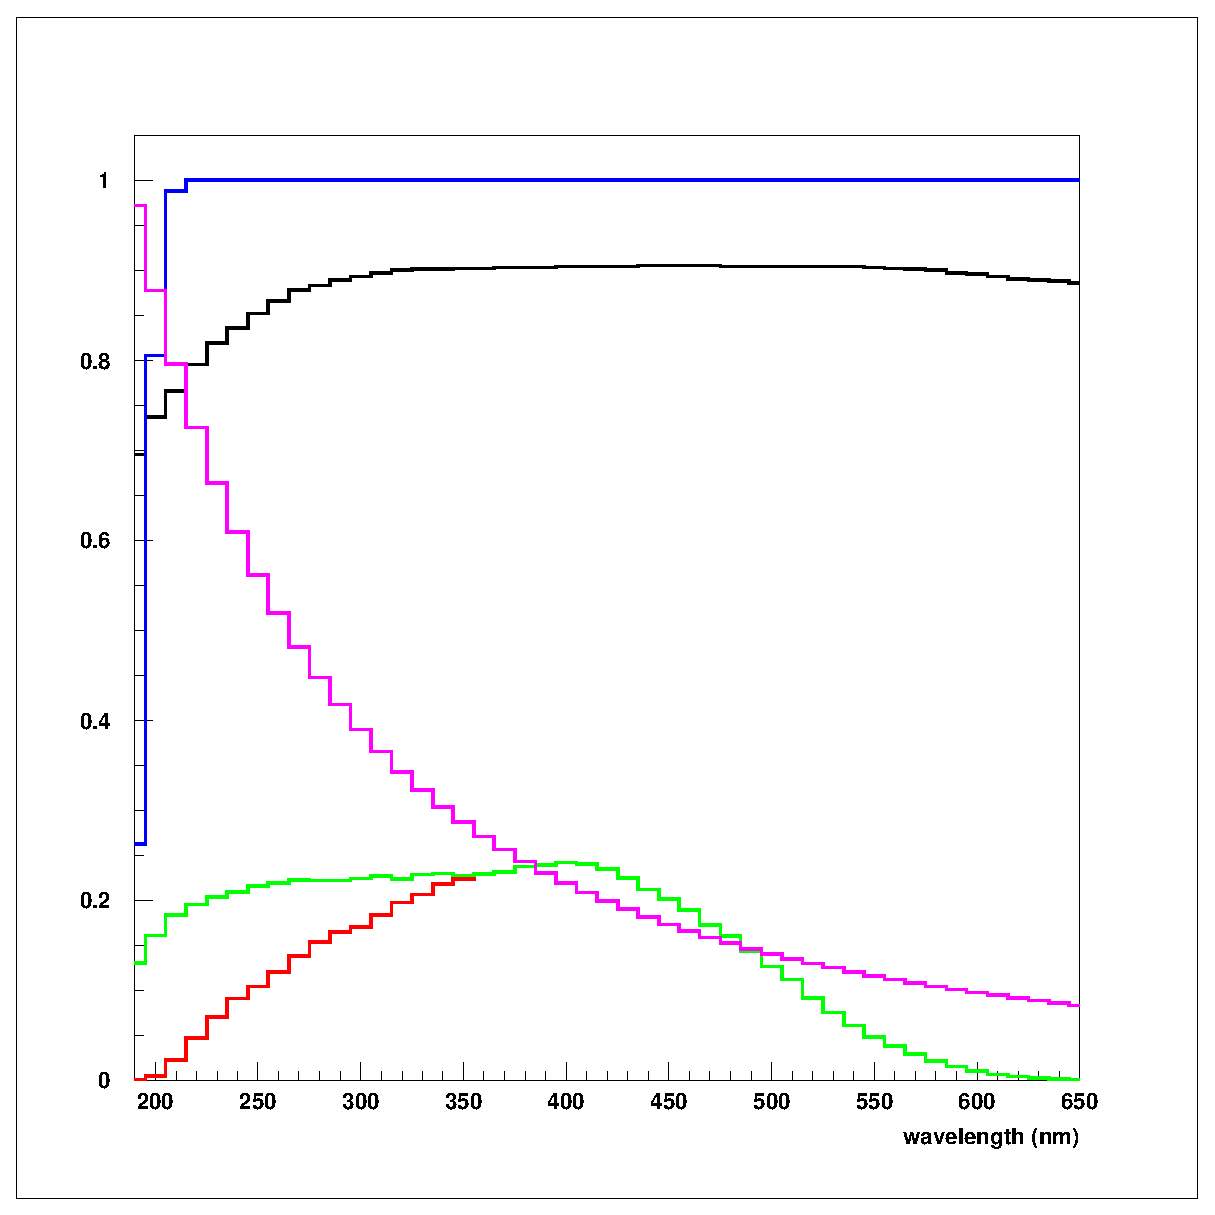
\includegraphics[height=12cm,angle=0]{MC-simulation/nphe_calc.eps}
\caption{\small{The optical properties of components of the HTCC
relative to maximizing the number of detected photoelectrons
as a function of photon wavelength.  The transparency of CO$_2$ is 
shown in blue, the reflectivity of aluminum in black, the photo-efficiency 
of a PMT with a UV glass window in red, and a quartz window in green. 
The magenta line represents the {\v C}erenkov spectrum (in arbitrary 
units).}}
\label{transparancy}
\end{figure}
%%%%%%%%%%%%%%%%%%%%%%%%%%%%%%%%%%%%%%%%%%%%%%%%%%%%%%%%%%%%%%%%%%%%%%

\subsubsection{Radiator Gas} 

The choice of radiator gas is CO$_2$, which has excellent optical 
transparency for wavelengths as low as 200~nm (see Fig.~\ref{transparancy}).
This is an important feature since the spectrum of {\v C}erenkov light is 
approximately $dn/d\lambda\propto 1/\lambda^2$.  The low index of 
refraction, $n \sim 1.00041$, corresponds to a pion threshold energy of 
4.7~GeV.  The trade-off is that fewer photons are produced at such low 
values of $n$. However, as will be seen, the number of collected photons 
is high enough to ensure a high detection efficiency. 

\subsubsection{Photomultiplier Tubes}

The use of 5-in photomultiplier tubes was chosen as the best match for the 
optical properties of the HTCC. This will be clear in the section on the 
photon spacial distributions at the face of the PMTs.  After consideration 
of PMTs from several manufacturers~\footnote{ElectronTubes, Burle, Hamamatsu, 
Photonis}, the Photonis XP4508 was chosen to have the best overall 
characteristics for our requirements. The window material is an important 
consideration.  Fig.~\ref{transparancy} compares the quantum efficiency of 
the Photonis XP4508 with UV glass and quartz windows. Clearly, the quartz 
window is superior in the low wavelength regime in which there are a large 
number of photons, and it matches the transparency range of the CO$_2$, as 
well as the reflectivity of the Al-MgF$_2$ mirror surfaces, which are also 
shown in Fig.~\ref{transparancy}.

The intensity and spectrum of \v{C}erenkov photons is given by the 
Frank-Tamm relation:

\begin{equation}
\frac{dN_{\gamma}}{dE} = \left( \frac{\alpha}{\hbar c} \right) Z^2 L
\left[1-(\frac{1}{n(E)\beta})^2 \right],
\end{equation} 

\noindent
where $Z$ is the particle charge, $n(E)$ is the index of refraction,
$L$ is particle trajectory length, and $(\frac{\alpha}{\hbar c}) = 
370$~eV$^{-1}$cm$^{-1}$. The expected number of obtained photoelectrons 
is then:
   
\begin{equation}
N_{ph.e.} = \int {}{}  \frac{dN_\gamma} {dE} \varepsilon(E)dE,
\end{equation}

\noindent
where $\varepsilon(E)$ is the detection efficiency of photons with energy 
$E$.  $\varepsilon(E)$ depends on the {\v C}erenkov gas transparency, 
reflection losses, quantum sensitivity of the PMT, and the probability of
missing the PMT because of geometry factors.  

The calculated mean number of photoelectrons per 1~cm of the trajectory is 
0.1477 for a UV glass PMT window and 0.2086 for a quartz PMT window.  The 
difference is essentially because of the fact that the {\v C}erenkov photon 
spectrum has an enhancement at low wavelengths -- see 
Fig.~\ref{transparancy}.  For our Monte Carlo simulations we assume quartz 
PMT windows.  The number of obtained photoelectrons was corrected for 
mirror imperfections and possible misalignments.  The correction 
coefficient, derived from the ratio of the Monte Carlo simulations and 
the experimental number of photoelectrons for the CLAS LTCC, was equal to 
2/3.

The shape of the PMT surface has also been considered, since the 
reflectivity of the PMT window, and thus the quantum efficiency, depends 
on the distribution of the angles of the photons relative to the PMT 
surface.   Fig.~\ref{angles} shows the simulated distribution of photon 
angles relative to the normal to the PMT surface for convex and flat 
windows, respectively.  It is seen that the distribution for the flat 
surface is closer to the surface normal than for the convex surface, and 
thus the flat surface quartz window was chosen as most appropriate for our 
purposes.

%%%%%%%%%%%%%%%%%%%%%%%%%%%%%%%%%%%%%%%%%%%%%%%%%%%%%%%%%%%%%%%%%%%%%%
\begin{figure}[htbp]
\centering
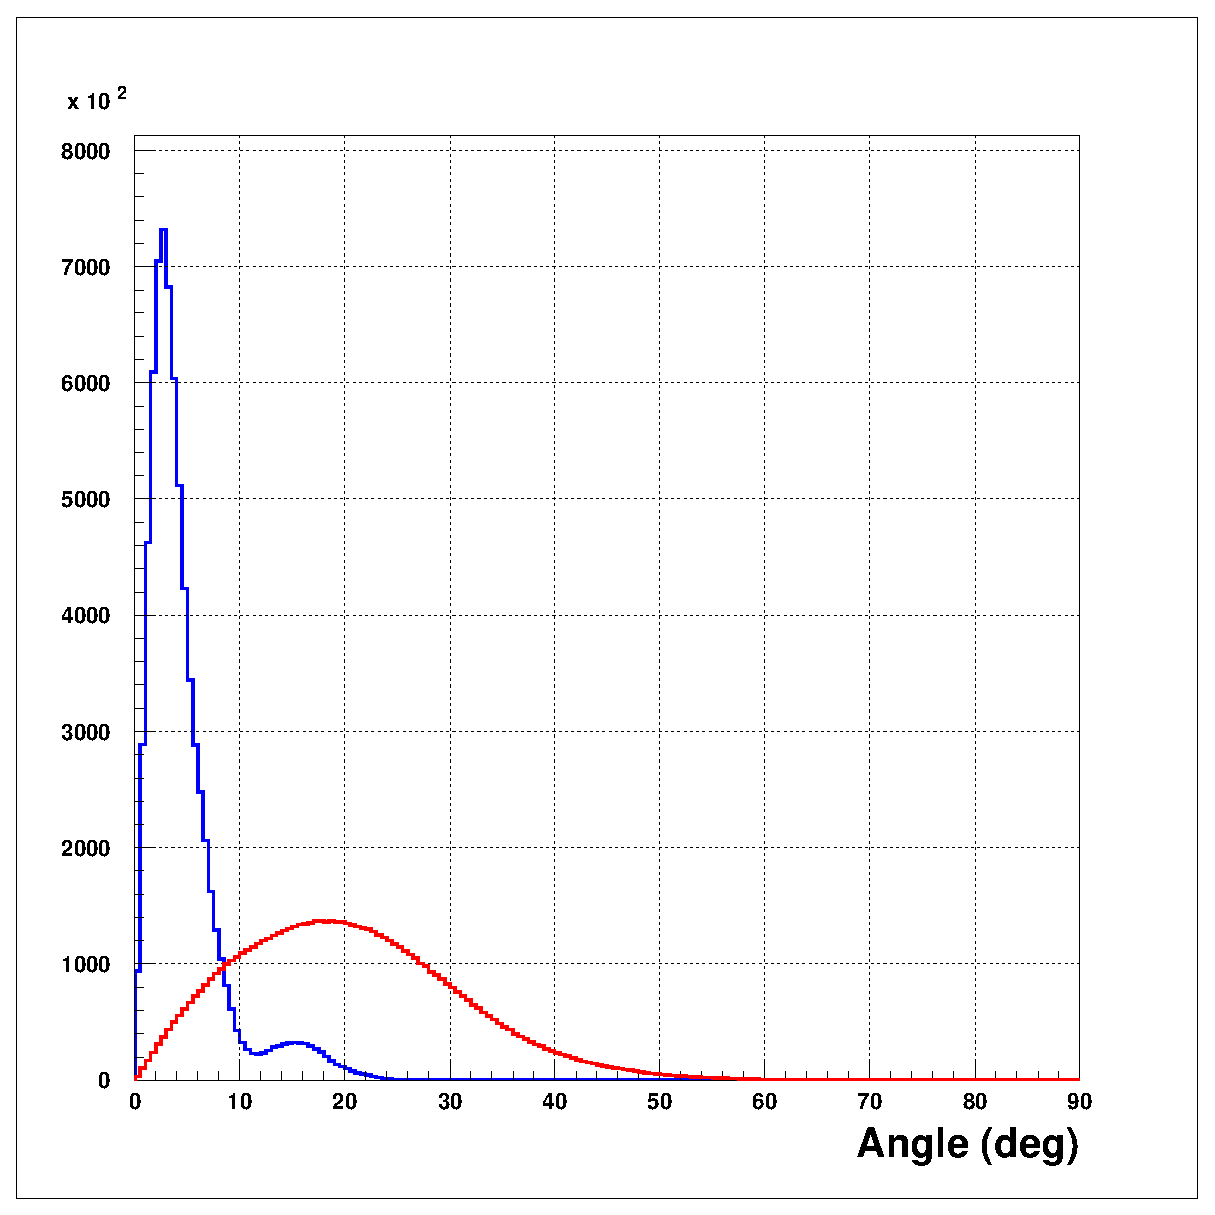
\includegraphics[height=8cm,angle=0]{MC-simulation/angles.eps}
\caption{\small{The simulated distribution of photon angles relative to 
the normal to the PMT surface for convex (red) and flat (blue) windows, 
respectively. The enhancement near the 15$^\circ$ (blue curve) is due to 
the photons, reflected off the Winston cone.}}
\label{angles}
\end{figure}
%%%%%%%%%%%%%%%%%%%%%%%%%%%%%%%%%%%%%%%%%%%%%%%%%%%%%%%%%%%%%%%%%%%%%%

\subsection{Distributions of Photons Incident on the PMT Faces}

Simulations were carried out to assess the HTCC response to scattered
electrons as a function of scattering angle in both $\theta$ and $\phi$.  
The results discussed in this section are for electrons of energy 2~GeV 
uniformly distributed in $d\Omega=\cos \theta d\theta d\phi$.  Each mirror 
is designed to direct the {\v C}erenkov light that impinges upon it onto 
the face of a specific PMT.  Fig.~\ref{four-tubes} shows the distribution 
of photons reaching PMTs in the PMT surface plane. 

The electrons originate from a target of length 10~cm, which is centered at 
the nominal central target position, with the full magnetic field 
configuration.  It is observed that the photons are constrained to circles 
of diameter approximately 16~cm, which is somewhat larger than the 11~cm 
PMT active diameters. Thus, light collection cones (Winston Cones) have 
been designed to redirect the photons that arrive outside of the 
photosensitive areas of the PMTs into the photosensitive areas.  All 
calculations were made for a Winston Cone window diameter of 7.5~in. 

%%%%%%%%%%%%%%%%%%%%%%%%%%%%%%%%%%%%%%%%%%%%%%%%%%%%%%%%%%%%%%%%%%%%%%
\begin{figure}[htbp]
\centering
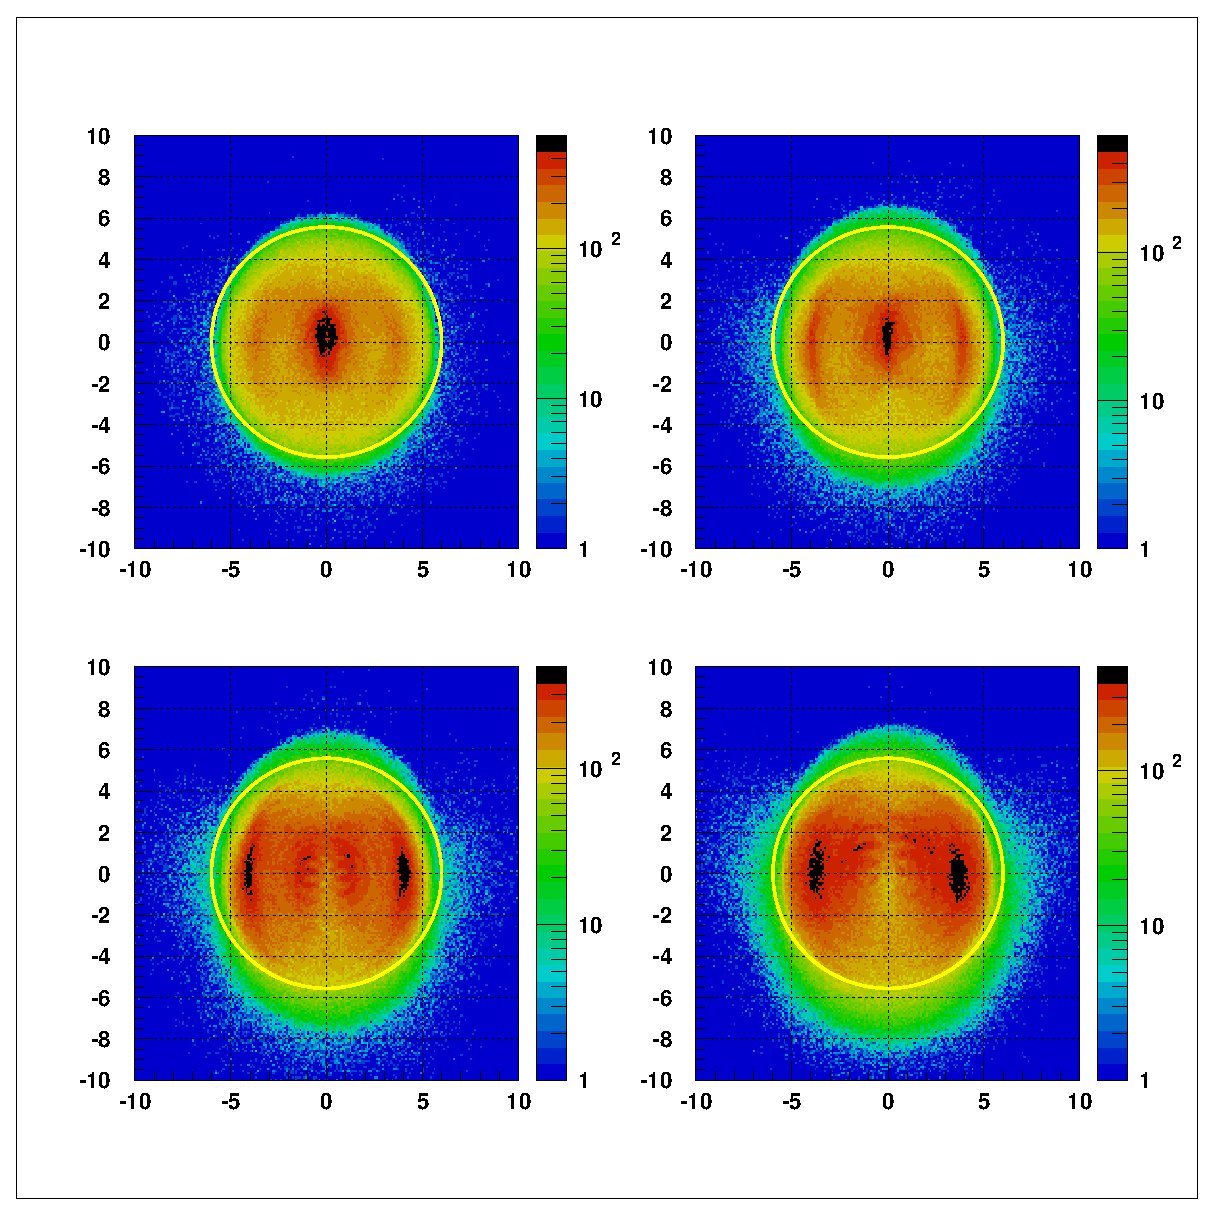
\includegraphics[height=14cm,angle=0]{MC-simulation/all_pmt.eps}
\caption{\small{The distribution of photons reaching the PMTs in the PMT
surface plane. Circles show the PMT size.}}
\label{four-tubes}
\end{figure}
%%%%%%%%%%%%%%%%%%%%%%%%%%%%%%%%%%%%%%%%%%%%%%%%%%%%%%%%%%%%%%%%%%%%%%

Fig.~\ref{nph-accept-2d} shows the overall acceptance in the number of 
photoelectrons as a function of $\theta$ and $\phi$ for one half of a 
sector, corresponding to the {\it standard} conditions described above. 
The results are the same for the 12 symmetrically placed half sectors 
corresponding to full $\Delta\phi = 2 \pi$.  Fig.~\ref{nph-vs-theta-phi} 
shows the projections of Fig.~\ref{nph-accept-2d} vs. $\theta$ and $\phi$,
respectively.  One observes that the mean number of photoelectrons is 
greater than 10 for scattered electrons in the angular range from about 
$5^\circ$ to $36^\circ$.  The $\theta$ dependence of the photoelectron 
number reflects the trajectory length dependence.

%%%%%%%%%%%%%%%%%%%%%%%%%%%%%%%%%%%%%%%%%%%%%%%%%%%%%%%%%%%%%%%%%%%%%%
\begin{figure}[htbp]
\centering
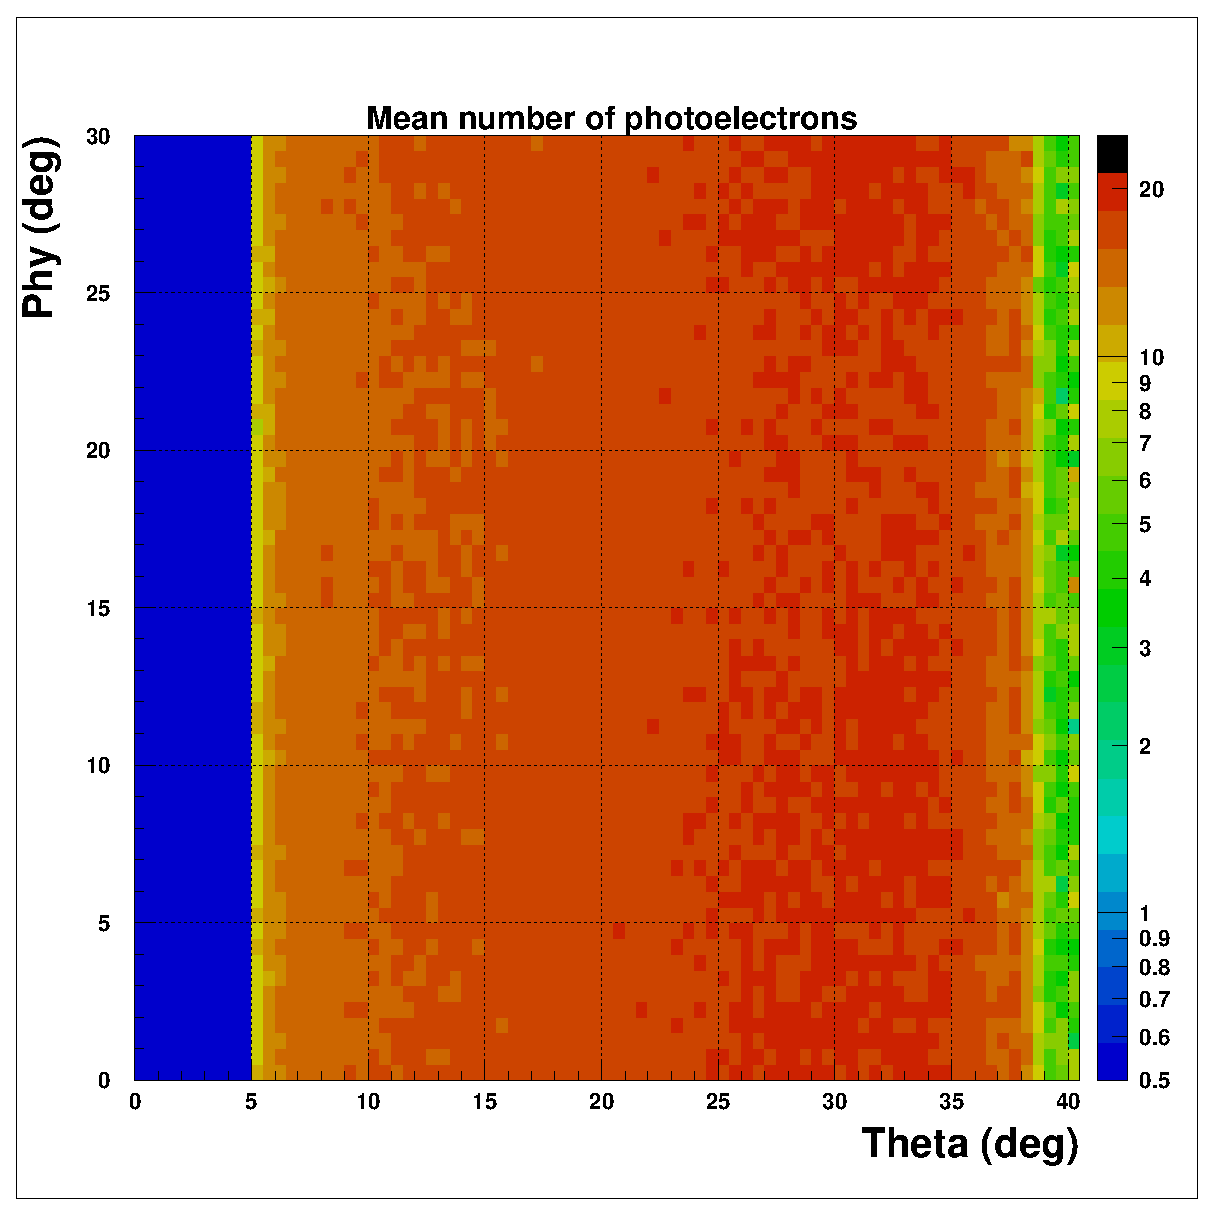
\includegraphics[height=12cm,angle=0]{MC-simulation/nph-accept-2d.eps}
\caption{\small{The overall acceptance in the number of photoelectrons
as a function of $\theta$ and $\phi$ for one half of a sector.}}
\label{nph-accept-2d}
\end{figure}
%%%%%%%%%%%%%%%%%%%%%%%%%%%%%%%%%%%%%%%%%%%%%%%%%%%%%%%%%%%%%%%%%%%%%%

%%%%%%%%%%%%%%%%%%%%%%%%%%%%%%%%%%%%%%%%%%%%%%%%%%%%%%%%%%%%%%%%%%%%%%
\begin{figure}[htbp]
\centering
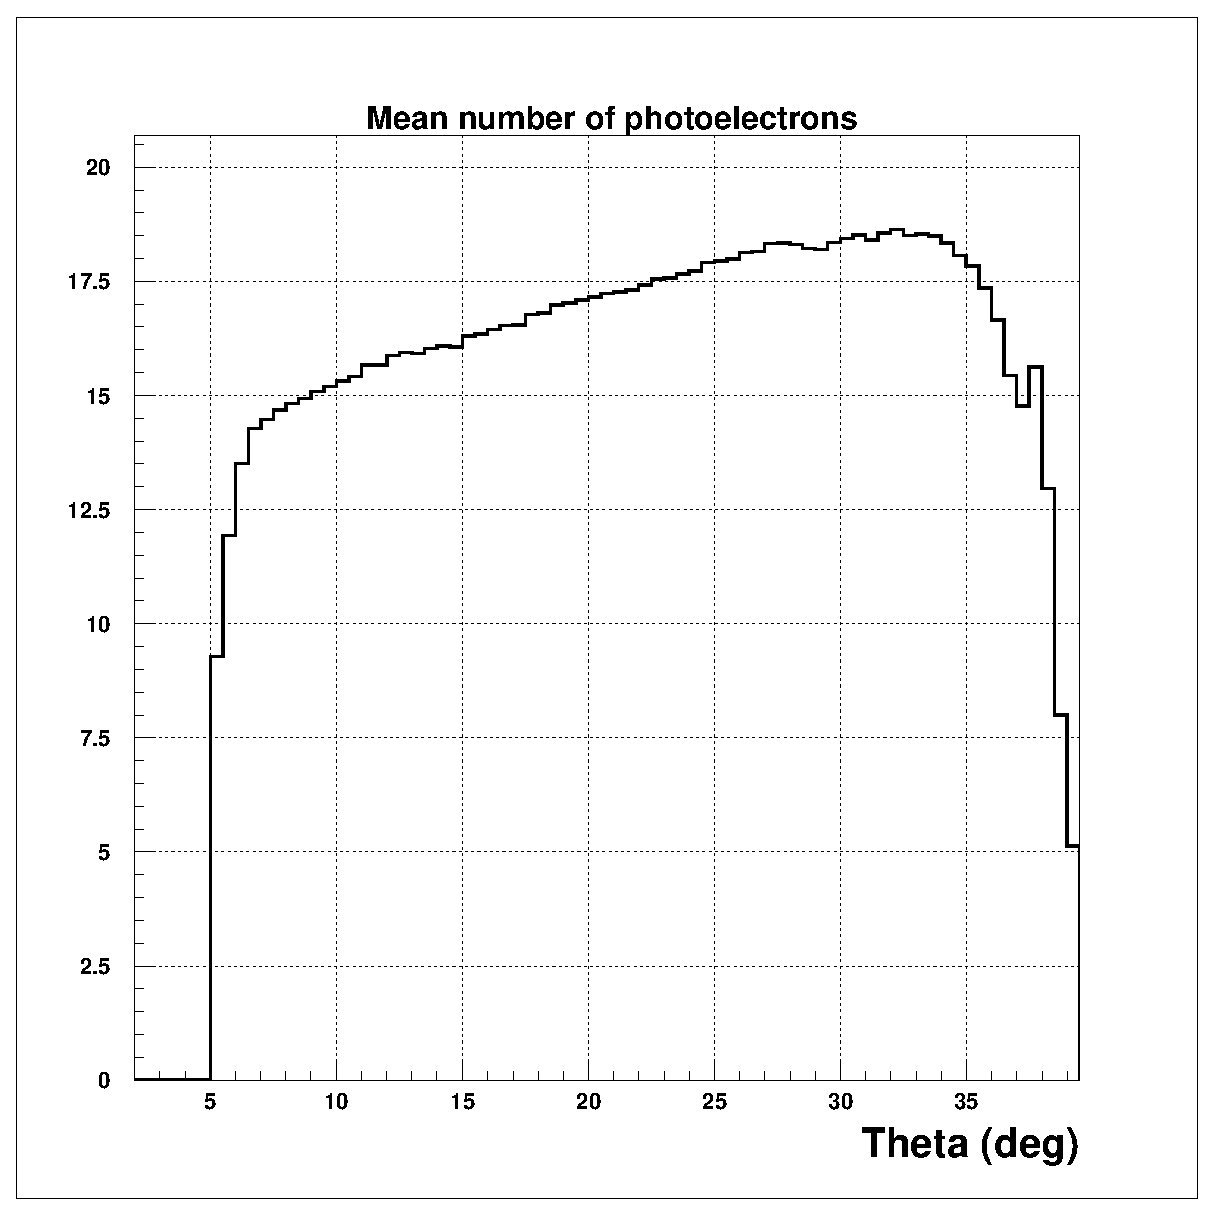
\includegraphics[height=8cm,angle=0]{MC-simulation/nph-vs-theta.eps}
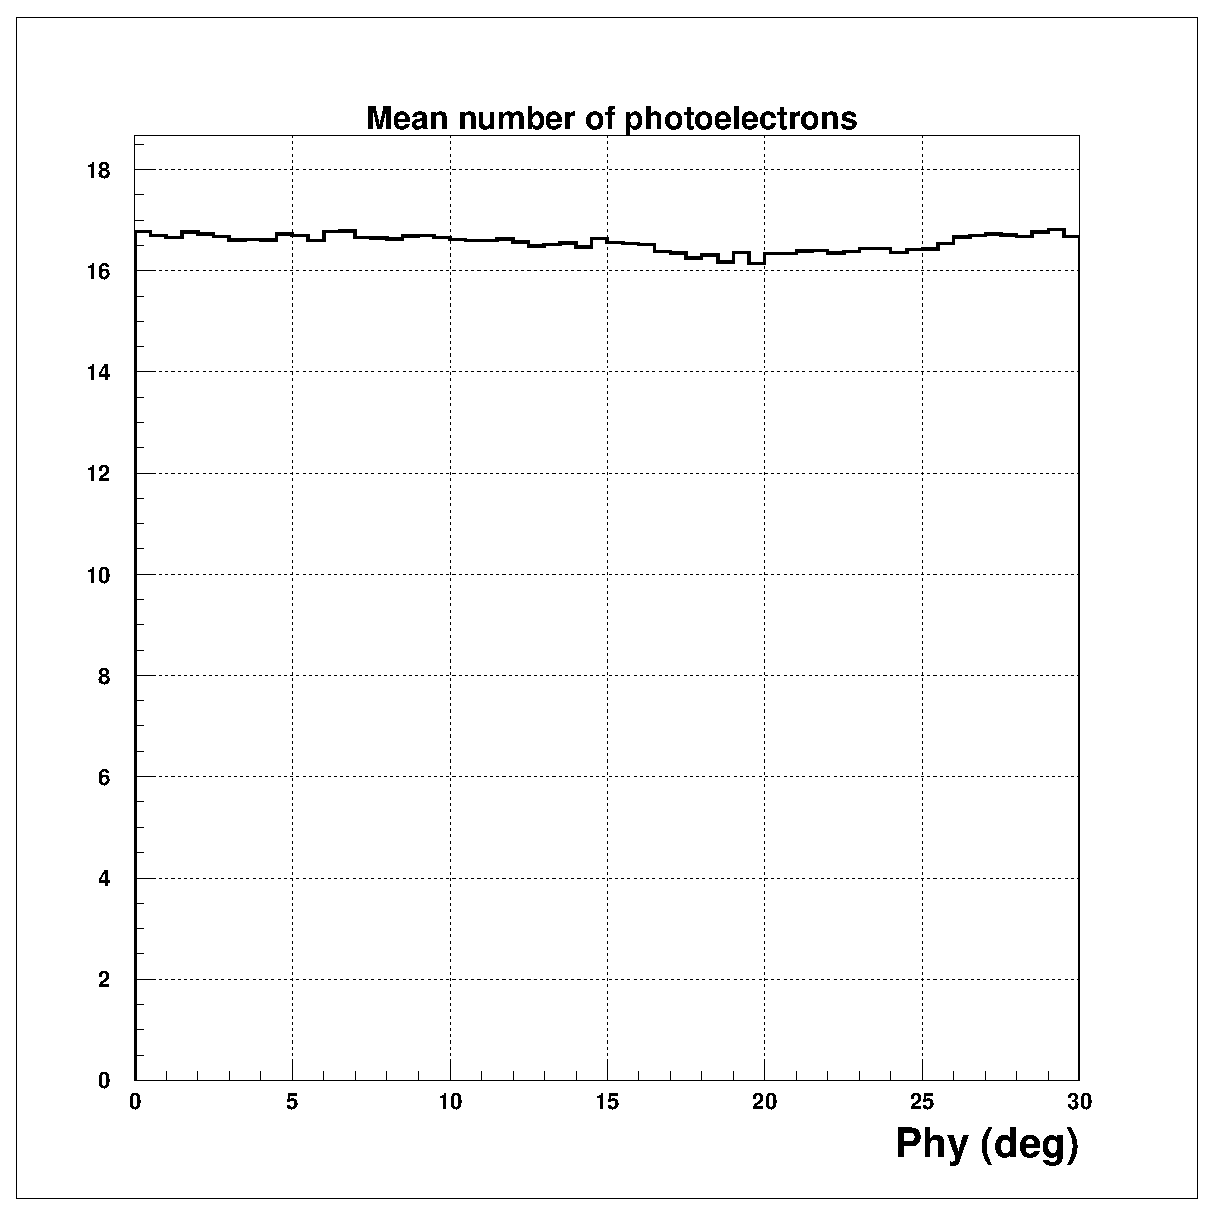
\includegraphics[height=8cm,angle=0]{MC-simulation/nph-vs-phi.eps}
\caption{\small{The projections of Fig.~\ref{nph-accept-2d} vs. 
$\theta$ and $\phi$, respectively.}}
\label{nph-vs-theta-phi}
\end{figure}
%%%%%%%%%%%%%%%%%%%%%%%%%%%%%%%%%%%%%%%%%%%%%%%%%%%%%%%%%%%%%%%%%%%%%%

%%%%%%%%%%%%%%%%%%%%%%%%%%%%%%%%%%%%%%%%%%%%%%%%%%%%%%%%%%%%%%%%%%%%%%
\begin{figure}[htbp]
\centering
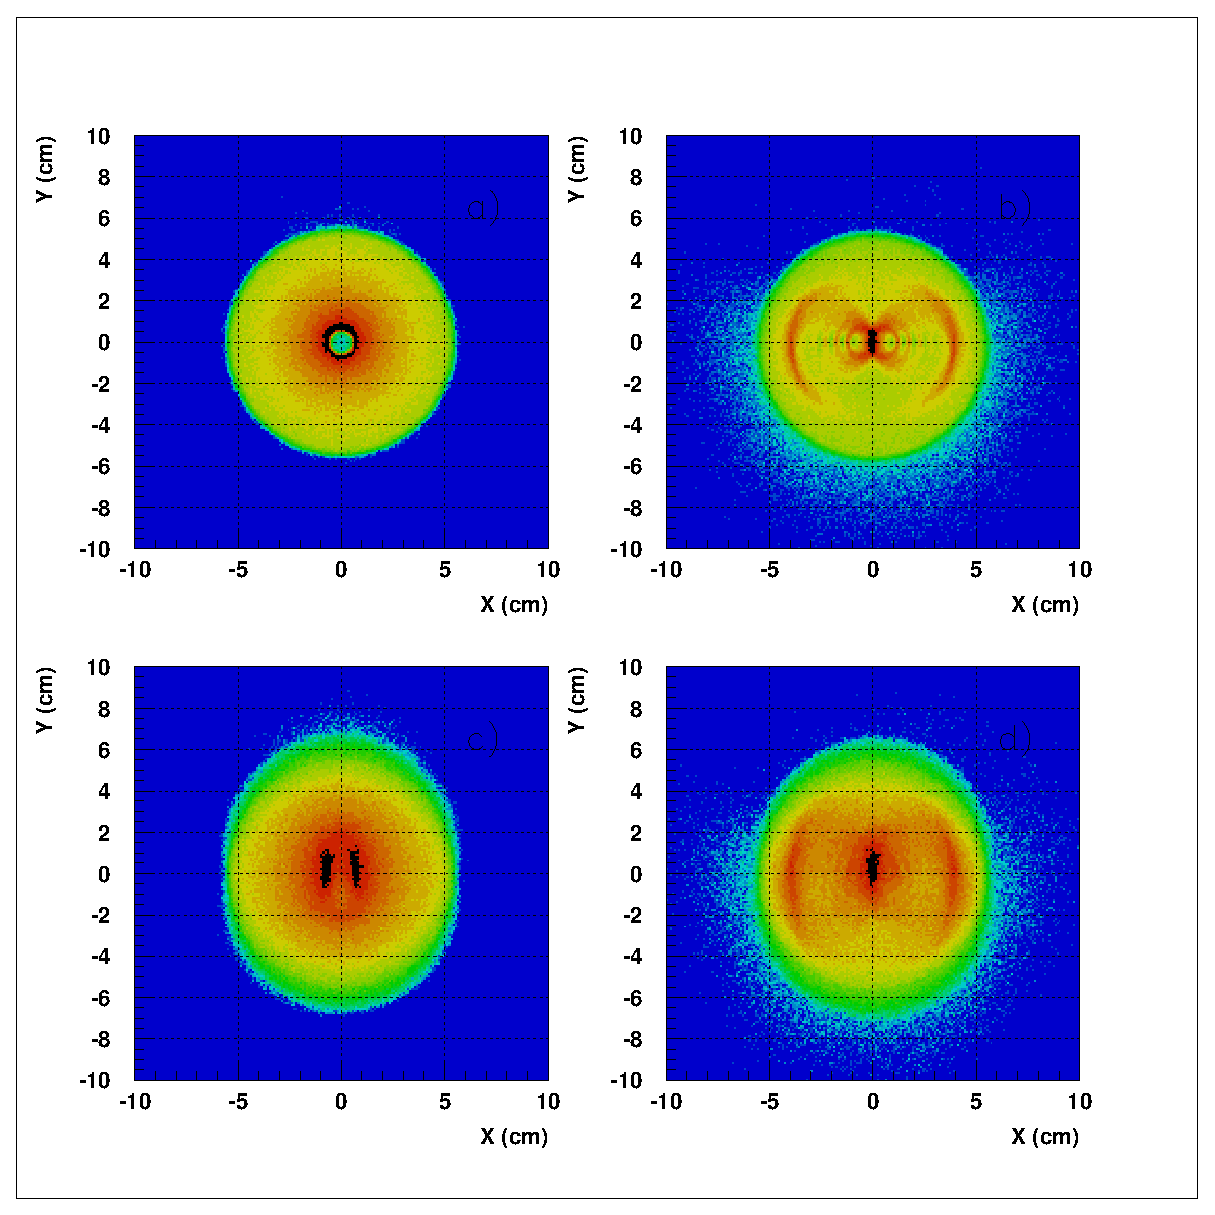
\includegraphics[height=12cm,angle=0]{MC-simulation/targ_field1.eps}
\caption{\small{The effect of the magnetic field and target length on the 
performance of the detector.  (a) is a point-like target, no magnetic field; 
(b) 10-cm target, no magnetic field; (c) and (d) are for a point-like target 
and a 10-cm target, respectively, in the 5~T solenoid magnetic field.}}
\label{fields}
\end{figure}
%%%%%%%%%%%%%%%%%%%%%%%%%%%%%%%%%%%%%%%%%%%%%%%%%%%%%%%%%%%%%%%%%%%%%%

The effect of the fields and target length on the performance of the 
detector are illustrated in Fig.~\ref{fields}a, b, c, and d, which show 
the distribution of photons on one PMT, number 2.  Case a) is a point-like 
target without magnetic field and case b) is a 10-cm target without magnetic 
field. Cases c) and d) are the point-like target and 10-cm target,
respectively, in the 5-T solenoid magnetic field.  Fig.~\ref{fields} shows 
that the distortions due to the target length and magnetic field are not 
very large, and the 7.5-inch diameter Winston Cone is an adequate choice
to collect all {\v C}erenkov light.

\subsection{Background Rates}

GEANT was used to estimate the background rate due to scattered electrons,
and electrons and positrons from secondary interactions with the detector 
materials.  Initial electrons with energy 11~GeV interact with the 5-cm 
liquid-hydrogen target in the 5-T solenoid magnetic field.  The beam pipe 
shielding starts from about 40~cm from the target.  The beam pipe shielding 
is between $2^\circ$ and $4^\circ$.  The PMT rates were reduced to the 
standard luminosity at 11~GeV, $10^{35}$~cm$^{-2}$s$^{-1}$.  The beam pipe 
shielding material was tungsten.

%%%%%%%%%%%%%%%%%%%%%%%%%%%%%%%%%%%%%%%%%%%%%%%%%%%%%%%%%%%%%%%%%%%%%%
\begin{figure}[htbp]
\centering
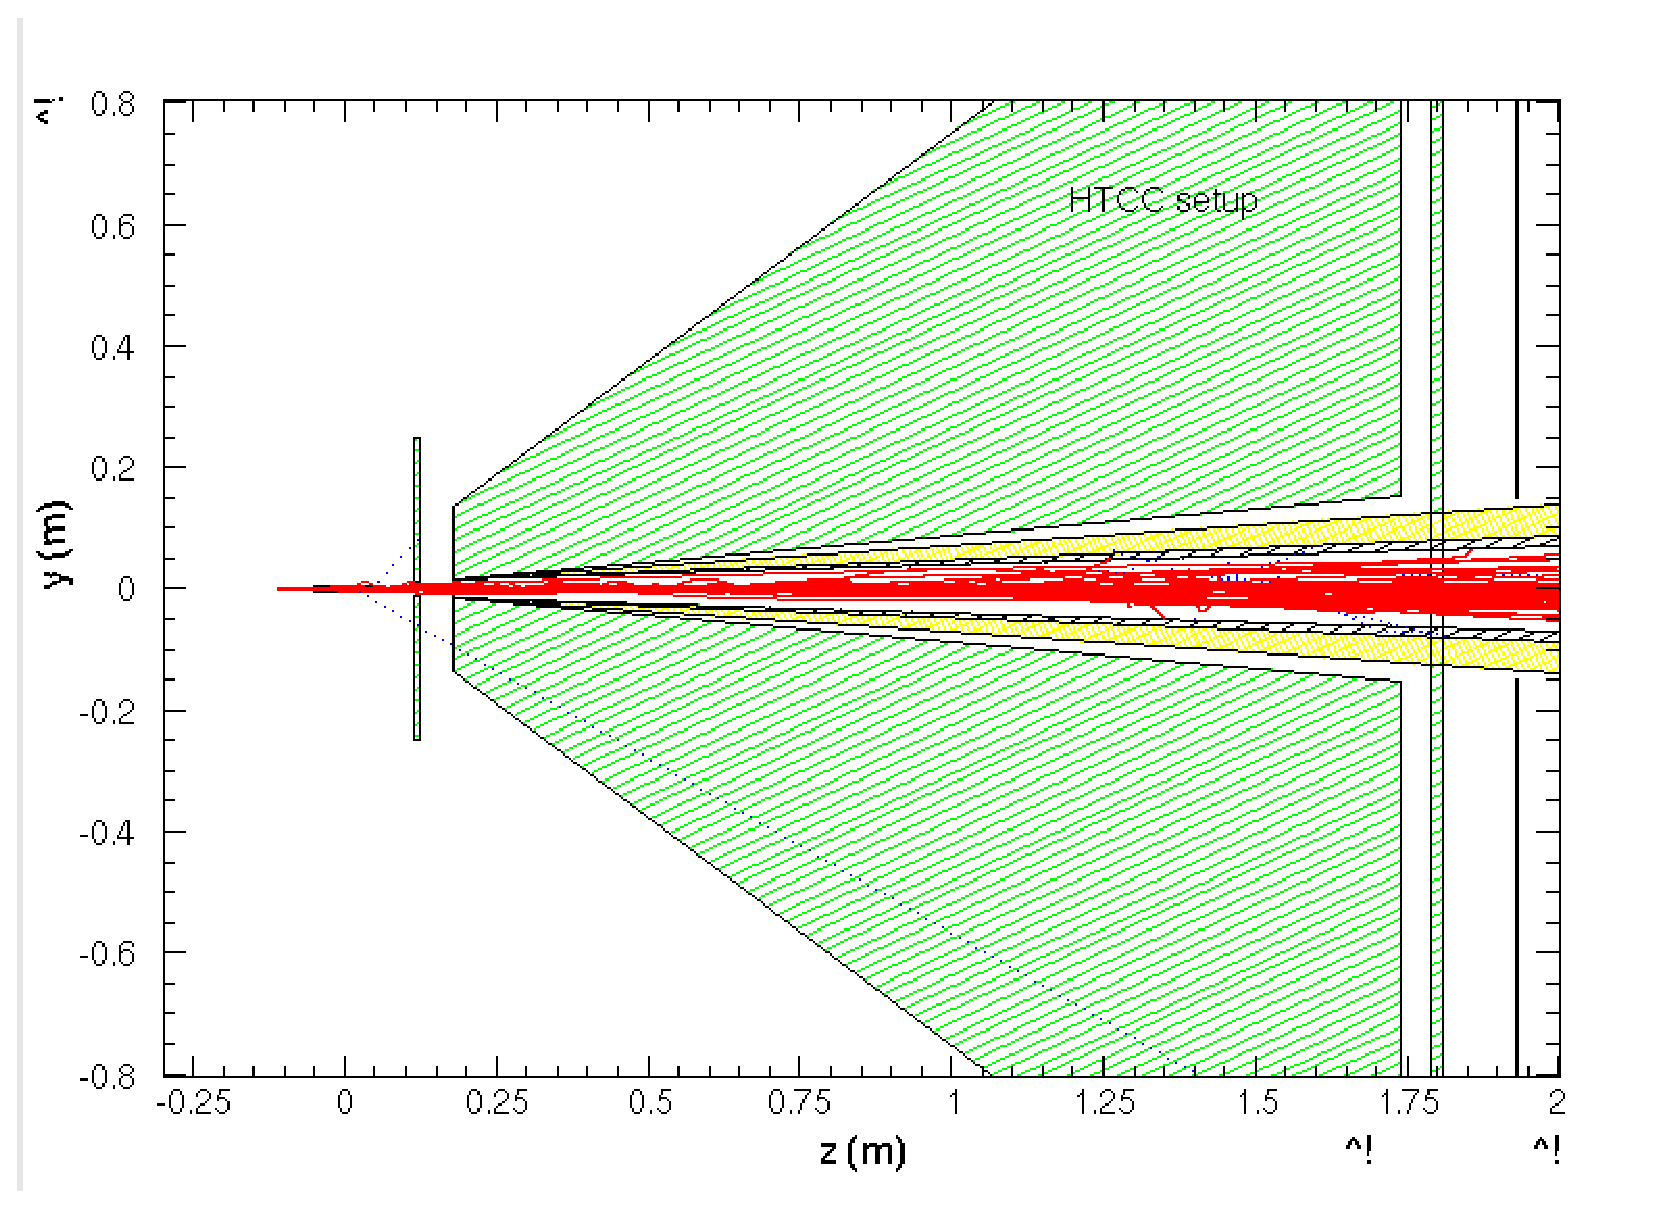
\includegraphics[height=6cm,angle=0]{MC-simulation/setup12.eps}
\includegraphics[height=6cm,angle=0]{MC-simulation/backgr1.eps}
\caption{\small{The experimental setup and background rates estimate.}}
\label{background1}
\end{figure}
%%%%%%%%%%%%%%%%%%%%%%%%%%%%%%%%%%%%%%%%%%%%%%%%%%%%%%%%%%%%%%%%%%%%%%

Fig.~\ref{background1} illustrates the beam pipe shielding setup and 
background PMT rates.  The highest rate is for the PMT at the lowest polar
angle.

For possible using the Inner Calorimeter for DVCS studies the other shielding
was designed. It covers the open angle from  $1^\circ$ to $1.5^\circ$,
and also the angle from  $5^\circ$ to $5.5^\circ$ . The setup and the
estimated background rate in this case is shown  in Fig.~\ref{background2}.
The background rate is a bit higher in this case, but
it can be easily handled by the data acquisition system.

 
%%%%%%%%%%%%%%%%%%%%%%%%%%%%%%%%%%%%%%%%%%%%%%%%%%%%%%%%%%%%%%%%%%%%%%
\begin{figure}[htbp]
\centering
\includegraphics[height=6cm,angle=0]{MC-simulation/dvcs12setup.eps}
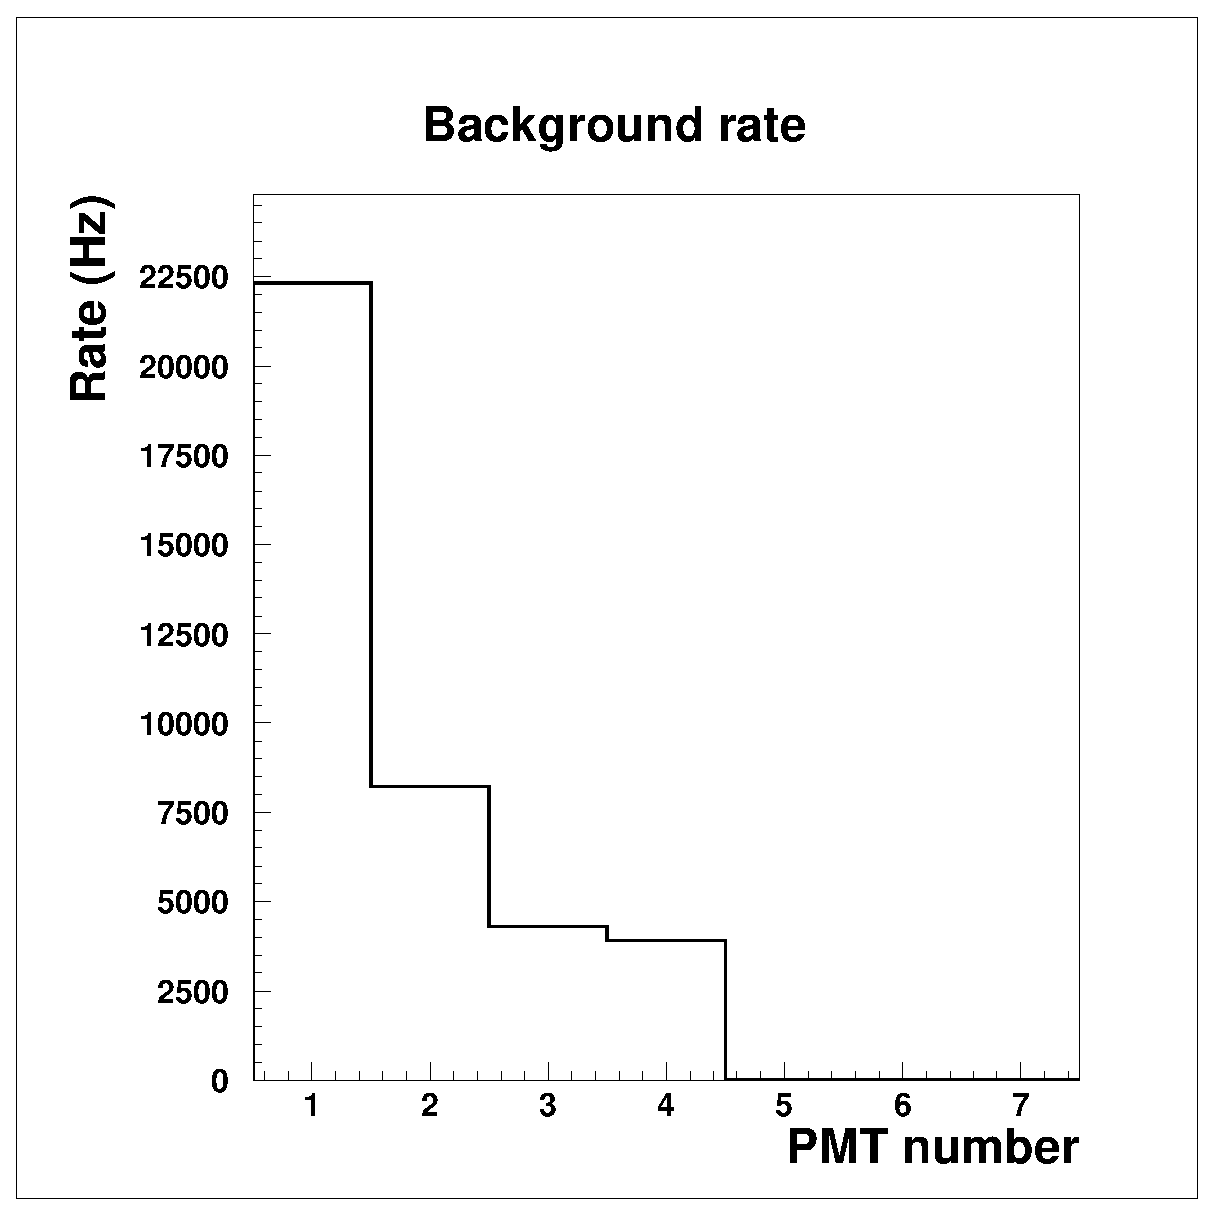
\includegraphics[height=6cm,angle=0]{MC-simulation/backgr2.eps}
\caption{\small{DVCS12 setup and background rates estimate.}}
\label{background2}
\end{figure}
%%%%%%%%%%%%%%%%%%%%%%%%%%%%%%%%%%%%%%%%%%%%%%%%%%%%%%%%%%%%%%%%%%%%%%

%%%%%%%%%%%%%%%%%%%%%%%%%%%%%%%%%%%%%%%%%%%%%%%%%%%%%%%%%%%%%%%%%%%%%%
%\begin{figure}[htbp]
%\centering
%\includegraphics[height=6cm,angle=0]{MC-simulation/dvcs12setup.eps}
%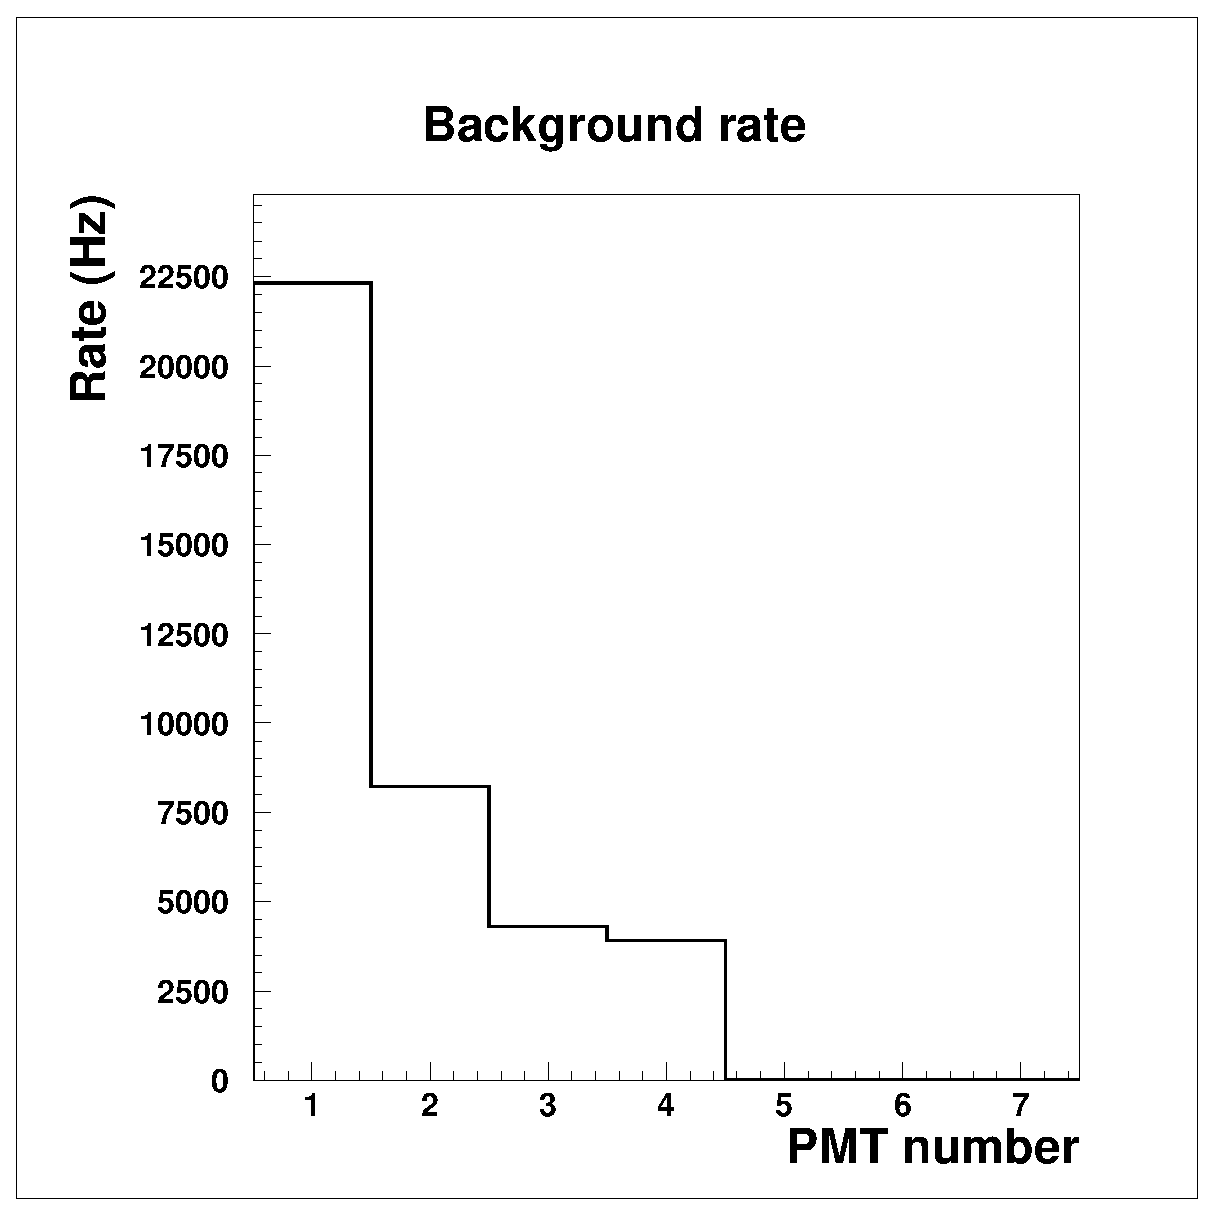
\includegraphics[height=6cm,angle=0]{MC-simulation/backgr2.eps}
%\caption{\small{The experimental setup and background rate estimate 
%(case 2).}}
%\label{background2}
%\end{figure}
%%%%%%%%%%%%%%%%%%%%%%%%%%%%%%%%%%%%%%%%%%%%%%%%%%%%%%%%%%%%%%%%%%%%%%

%%%%%%%%%%%%%%%%%%%%%%%%%%%%%%%%%%%%%%%%%%%%%%%%%%%%%%%%%%%%%%%%%%%%%%
\begin{figure}[htbp]
\centering
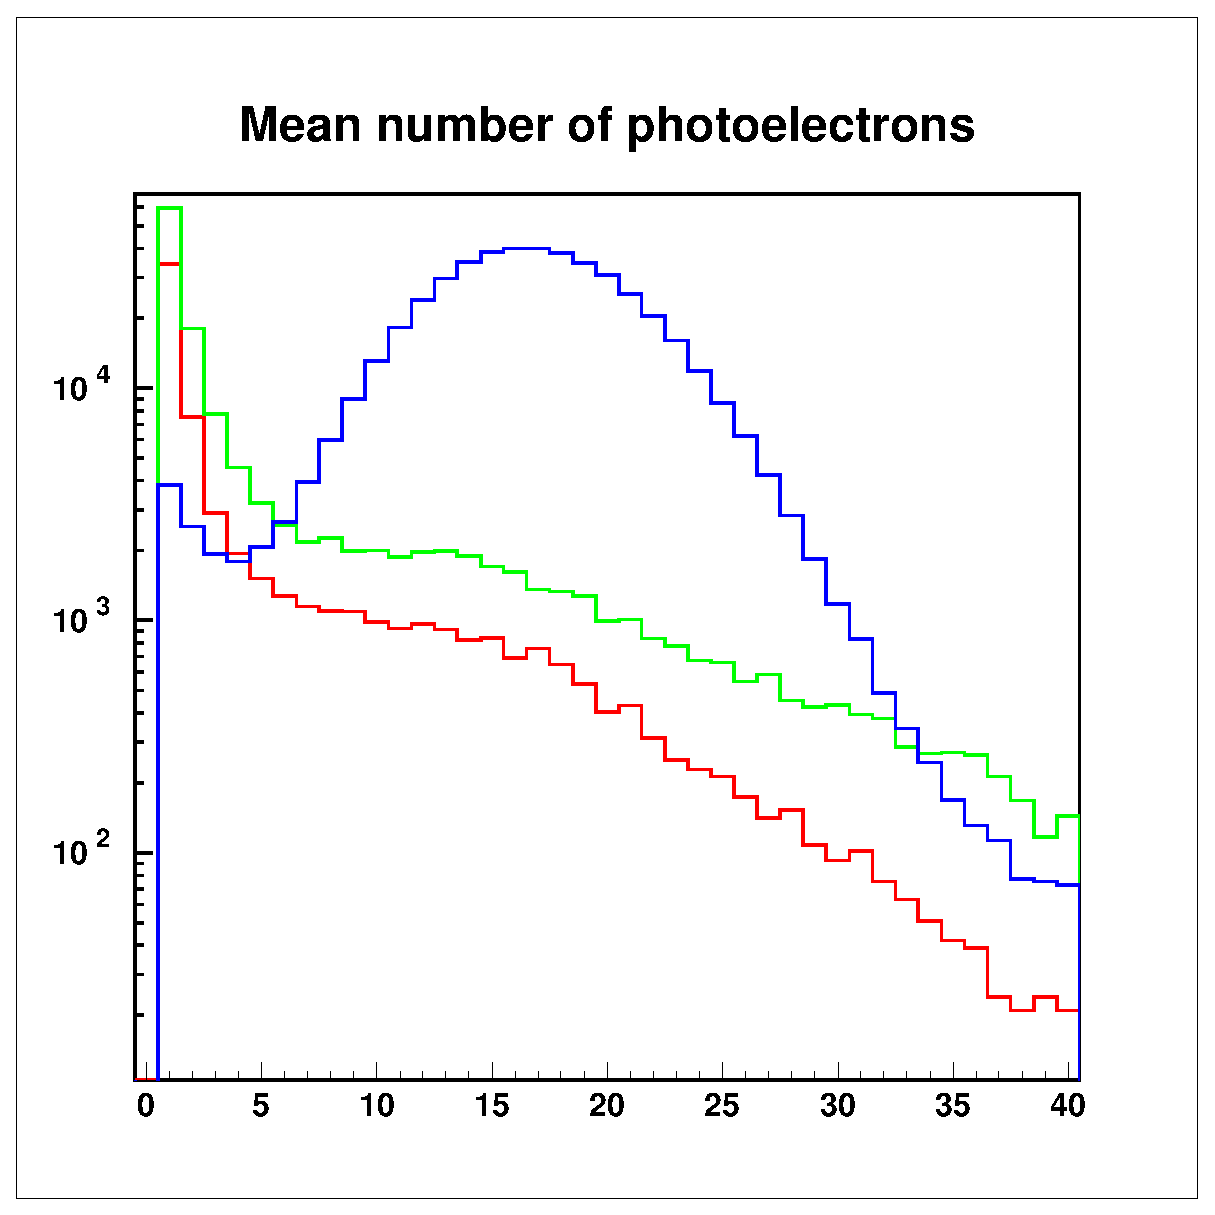
\includegraphics[height=8cm,angle=0]{MC-simulation/pions_nphe.eps}
\caption{\small{The amplitude distribution of detected pions (in 
photoelectrons) for 2~GeV (red curve) and 4~GeV pions (green curve).
The blue curve shows the amplitude distribution for the detected electrons.}}
\label{pions_nphe}
\end{figure}
%%%%%%%%%%%%%%%%%%%%%%%%%%%%%%%%%%%%%%%%%%%%%%%%%%%%%%%%%%%%%%%%%%%%%%

%%%%%%%%%%%%%%%%%%%%%%%%%%%%%%%%%%%%%%%%%%%%%%%%%%%%%%%%%%%%%%%%%%%%%%
\begin{figure}[htbp]
\centering
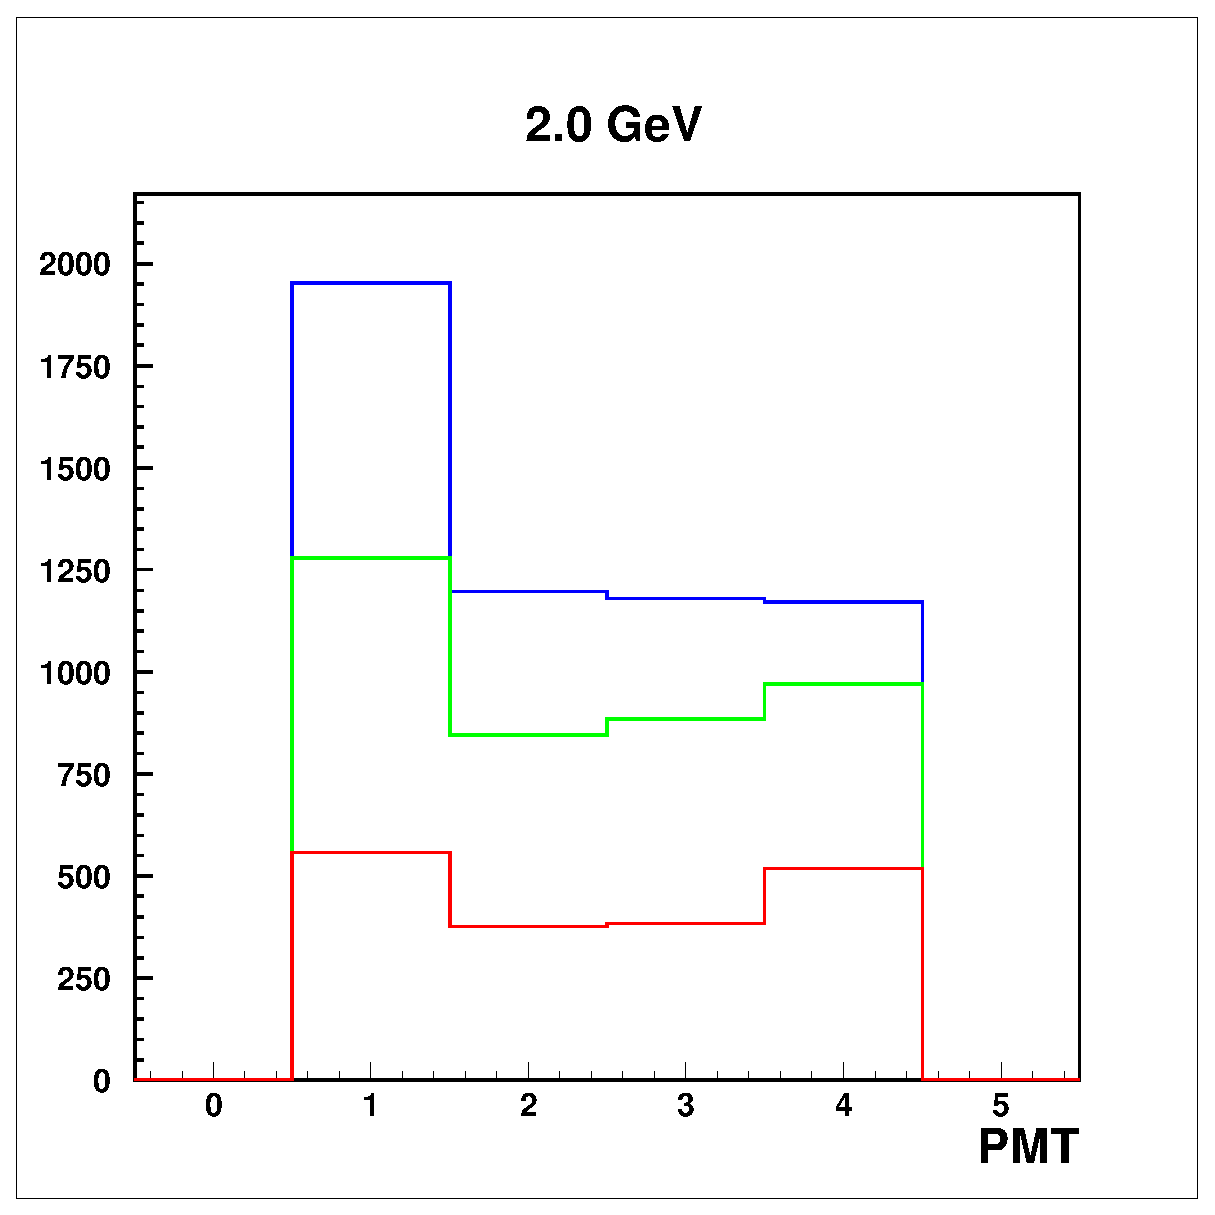
\includegraphics[height=8cm,angle=0]{MC-simulation/pions1a.eps}
\includegraphics[height=8cm,angle=0]{MC-simulation/pions1b.eps}
\caption{\small{The simulated pion rejection factor of pions to electron 
identification for initial 2~GeV and 4~GeV pions.  The different curves 
represent different amplitude thresholds: red is for one photoelectron, 
green for two photoelectrons, and blue for three photoelectrons.}}
\label{pion-rejection}
\end{figure}
%%%%%%%%%%%%%%%%%%%%%%%%%%%%%%%%%%%%%%%%%%%%%%%%%%%%%%%%%%%%%%%%%%%%%%

The $\pi/e$ rejection factor is very important for the {\v C}erenkov 
detector.  Pions can produce $\delta$-electrons, which can be detected in 
the HTCC.  However, the amplitude distribution of such events is low. 
Fig.~\ref{pions_nphe} shows the amplitude distribution of detected pions 
(in photoelectrons) for 2~GeV (blue curve) and 4~GeV pions (red curve).

Fig.~\ref{pion-rejection} shows the $\pi/e$ rejection factor, calculated as 
the ratio of electron to pion detection efficiency, for 2~GeV and 4~GeV 
pions.  The red line shows the $\pi/e$ rejection factor with a threshold 
of one photoelectron, green - two photoelectrons, and blue - three 
photoelectrons.  The $\pi/e$ rejection factor can be as high as 500 even 
for high momentum pions.  It must be noted that the electron detection 
efficiency is still very high at thresholds up to three photoelectrons: 
99.99\% for two photoelectrons and 99.90\% for three photoelectrons.

\subsection{Timing Parameters}

GEANT can be used to estimate the trajectory length and the ray-tracing 
length difference for {\v C}erenkov photons for different PMTs.  The 
detection time difference is shown in Fig.~\ref{timing}.  It is evident 
that HTCC signals can be used for good time-of flight measurements, because 
even at larger $\theta$ angles, the timing is within $\pm$0.2~ns.

%%%%%%%%%%%%%%%%%%%%%%%%%%%%%%%%%%%%%%%%%%%%%%%%%%%%%%%%%%%%%%%%%%%%%%
\begin{figure}[htbp]
\centering
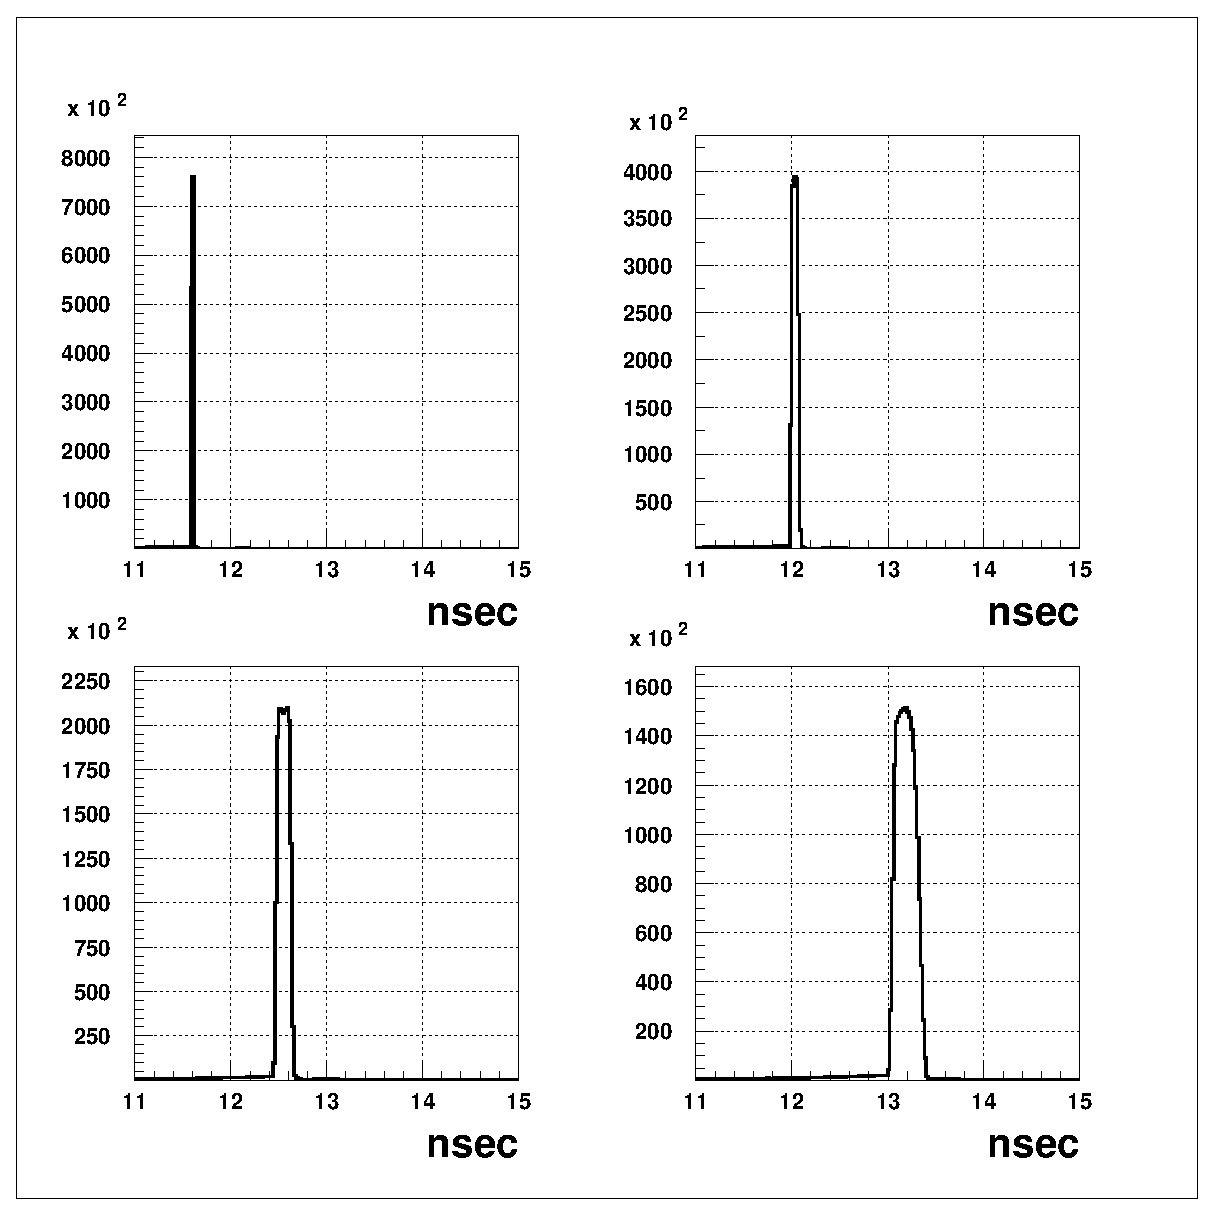
\includegraphics[height=10cm,angle=0]{MC-simulation/timing.eps}
\caption{\small{ The detection time difference for different HTCC PMTs.}}
\label{timing}
\end{figure}
%%%%%%%%%%%%%%%%%%%%%%%%%%%%%%%%%%%%%%%%%%%%%%%%%%%%%%%%%%%%%%%%%%%%%%

\section{PMT Studies}

\subsection{PMT Magnetic Shielding Studies}

The PMTs of the HTCC will be located in a region in which there will 
be a significant magnetic field, primarily from the solenoid magnet 
that surrounds the target and central detector system.  The field 
varies considerably with distance from the solenoid, with a maximum 
value of as much as 50~G in the region of the PMTs closest to the 
solenoid.  To give an idea of the magnitude of the problem, we note 
that for tests we have carried out, the PMT gain is reduced by a factor
of two for a magnetic field of 0.4~G perpendicular to the PMT axis    
and 1.3~G parallel to the PMT axis.  The standard PMT magnetic shield 
that can be obtained from the PMT manufacturer is totally inadequate to 
reduce the ambient field to even these levels, so that it is necessary 
to custom design a magnetic shielding system appropriate for the
{\tt CLAS12} HTCC configuration.  The design is being carried out with 
the aid of the TOSCA magnetic field program. 

Figs.~\ref{lin_r}, \ref{log_r}, \ref{lin_z}, and \ref{log_z} present the 
residual magnetic field at the PMT axis for a standard single-layer PMT 
magnetic shield for three values of the field: 50~G, 40~G, and 30~G, 
with the direction of the magnetic field perpendicular and parallel to the 
PMT axis (linear and logarithmic $y$-scales are shown).  In the first 
case, the residual magnetic field inside the PMT volume is around 8~G, 
2~G, and 1~G for a magnetic field of 50~G, 40~G, and 30~G, respectively. 
For the second case (the field is along the PMT axis), the field residual 
is significantly higher.  The residual magnetic field inside the PMT volume 
is around 30~G, 10~G, and 1-2~G for magnetic fields of 50~G, 40~G, and 
30~G, respectively.  We may conclude from this calculation that:

\begin{itemize}
\item We need additional magnetic shielding to suppress the residual 
magnetic field to the level of 0.5~G;
\item The residual field is significantly (several times) higher when 
the magnetic field is directed along the PMT axis;
\item The shielding needs to extend beyond the PMT window for at least 
one PMT diameter.
\end{itemize}

We modeled three-layer magnetic shielding configurations using the 
TOSCA program.  Fig.~\ref{3layers} shows the residual field for 3 
different configurations with cylindrical PMT magnetic shielding with 
the magnetic field directed along the PMT axis.  The magnetic shielding 
has 1-mm thickness for every layer.  For these studies, the following
conditions apply:

\begin{itemize}
\item Single layer tube made of co-netic $\mu$-metal (shown in black),
\item Two layers made of netic and co-netic $\mu$-metals (shown in red),
\item Three layers made of netic, co-netic, and co-netic $\mu$-metals 
(shown in blue).
\end{itemize}

The residual magnetic field with the three-layer shielding is below 1~G 
in the region $\pm$5~cm, which is inside the specifications for the
magnetic field parallel to the PMT axis.  The perpendicular field will 
be several times lower, based on our calculations with the standard PMT 
magnetic shielding.

%%%%%%%%%%%%%%%%%%%%%%%%%%%%%%%%%%%%%%%%%%%%%%%%%%%%%%%%%%%%%%%%%%%%%%%%
\begin{figure}
\hspace{0.5cm}
\begin{centering}
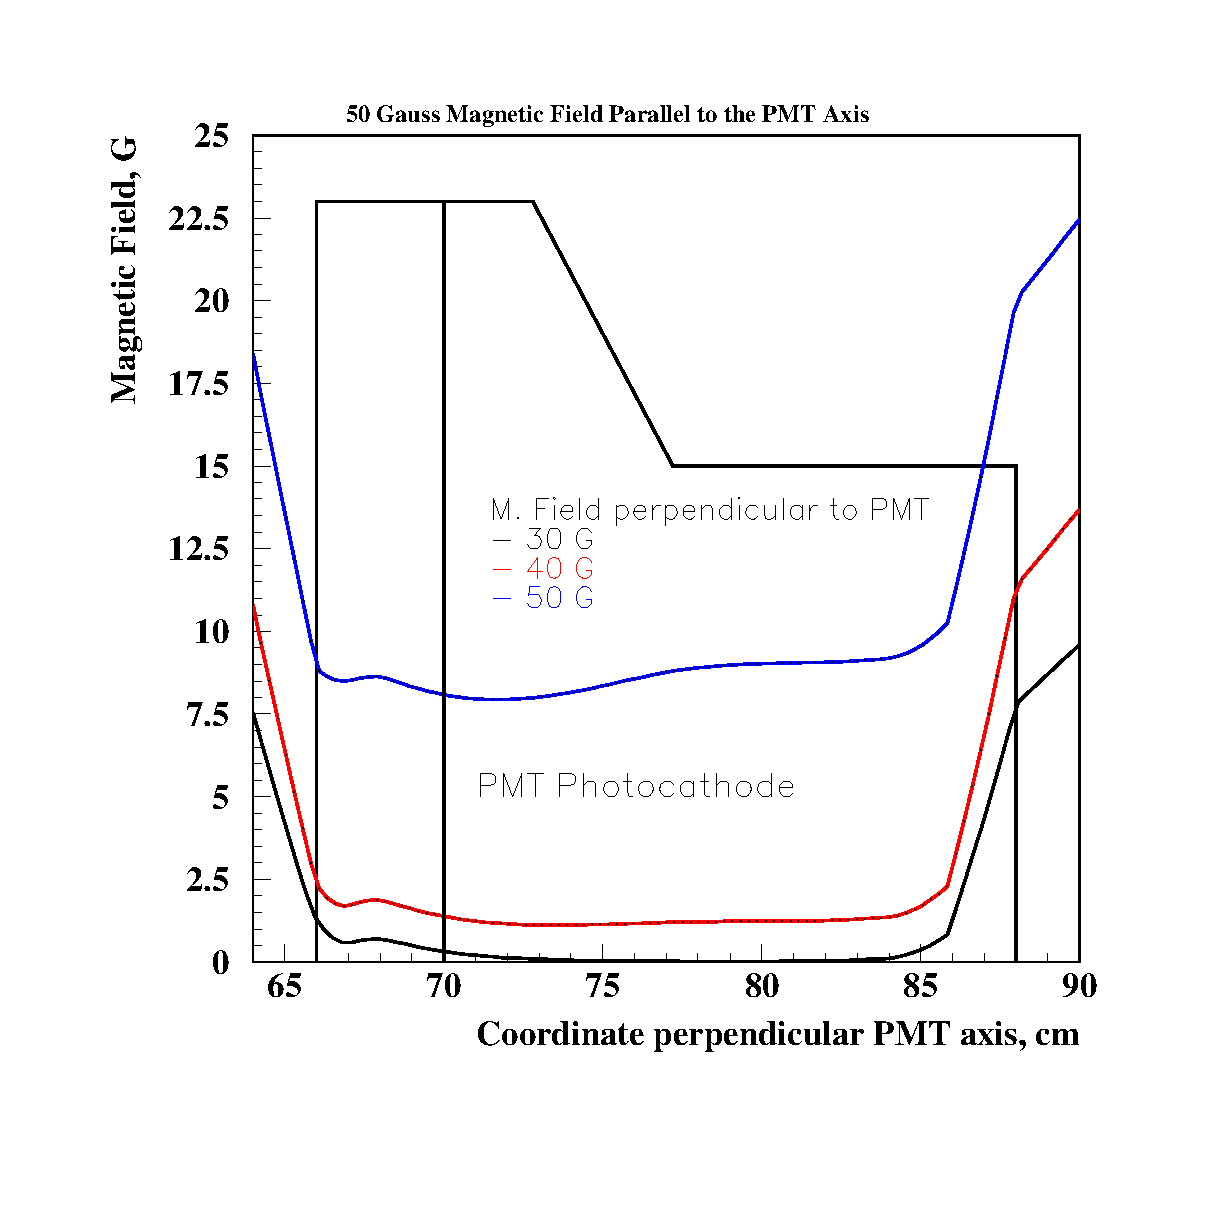
\includegraphics[height=7.5cm]{Magnetic-shielding/shield_r_lin.eps}
\vspace{0.5cm}
\caption{\small{Standard single-layer PMT magnetic shielding (shown in 
black).  The magnetic field is perpendicular to the PMT axis.  The result 
with applied external fields of 50~G is shown in blue, 40~G in red, and 
30~G in black.  The PMT photocathode position is shown by the black 
vertical line.}}
\label{lin_r}
\end{centering}
\end{figure}
%%%%%%%%%%%%%%%%%%%%%%%%%%%%%%%%%%%%%%%%%%%%%%%%%%%%%%%%%%%%%%%%%%%%%%%%

%%%%%%%%%%%%%%%%%%%%%%%%%%%%%%%%%%%%%%%%%%%%%%%%%%%%%%%%%%%%%%%%%%%%%%%%
\begin{figure}
\hspace{0.5cm}
\begin{centering}
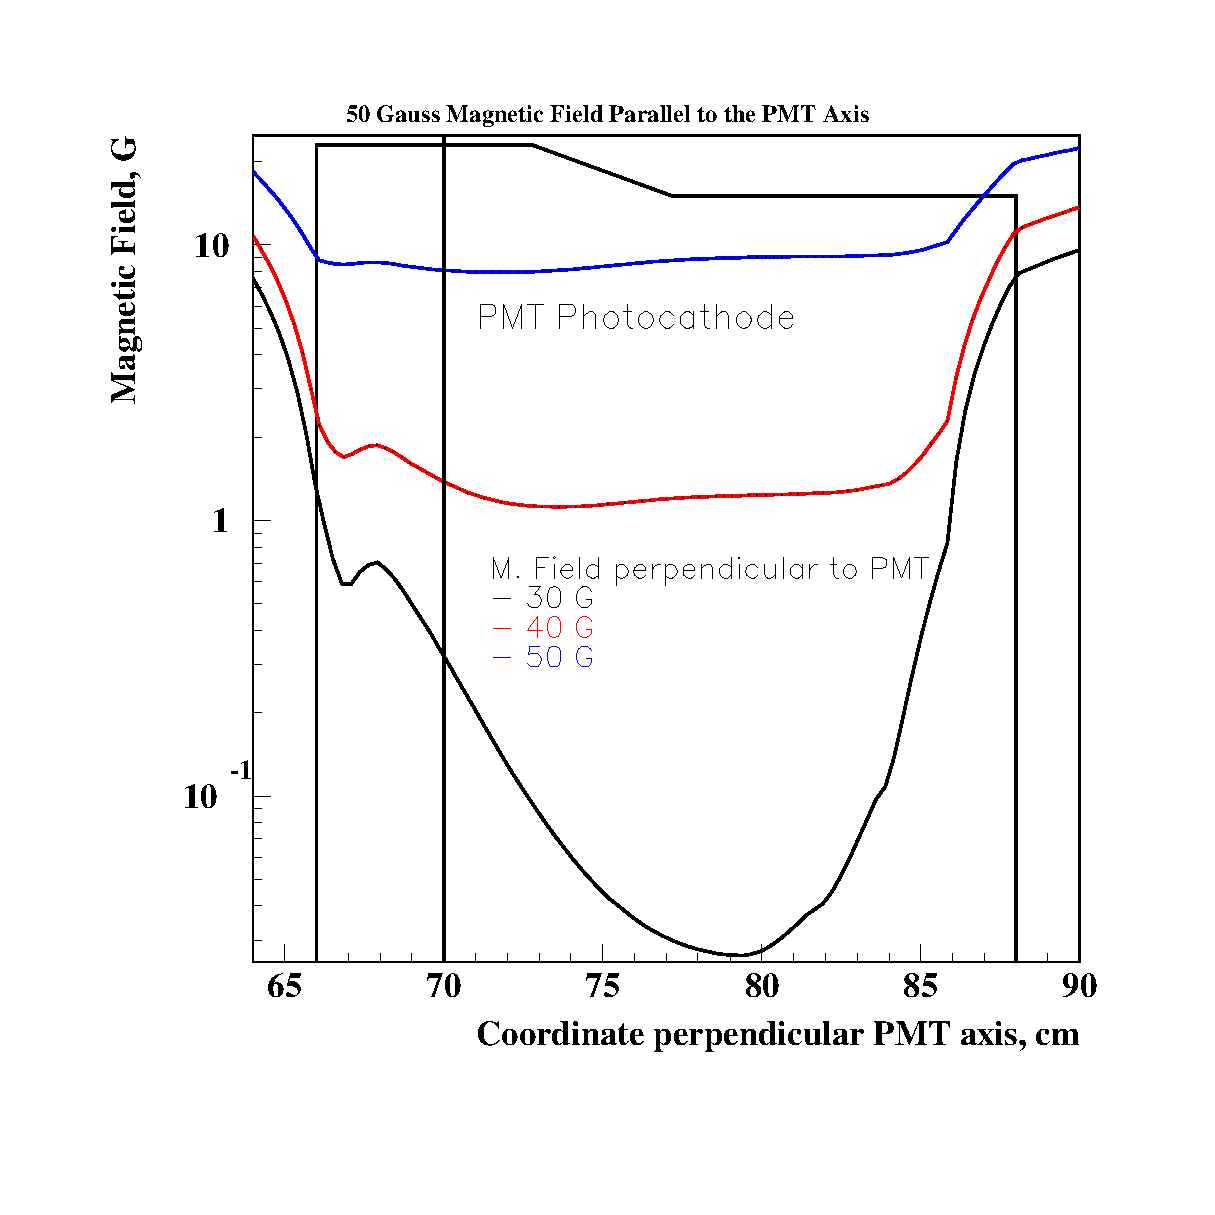
\includegraphics[height=7.5cm]{Magnetic-shielding/shield_r_log.eps}
\vspace{0.5cm}
\caption{\small{Same as in Fig.~\ref{lin_r} but with a logarithmic $y$-axis.
The PMT photocathode position is shown by the black vertical line.}}
\label{log_r}
\end{centering}
\end{figure}
%%%%%%%%%%%%%%%%%%%%%%%%%%%%%%%%%%%%%%%%%%%%%%%%%%%%%%%%%%%%%%%%%%%%%%%%

%%%%%%%%%%%%%%%%%%%%%%%%%%%%%%%%%%%%%%%%%%%%%%%%%%%%%%%%%%%%%%%%%%%%%%%%
\begin{figure}
\hspace{0.5cm}
\begin{centering}
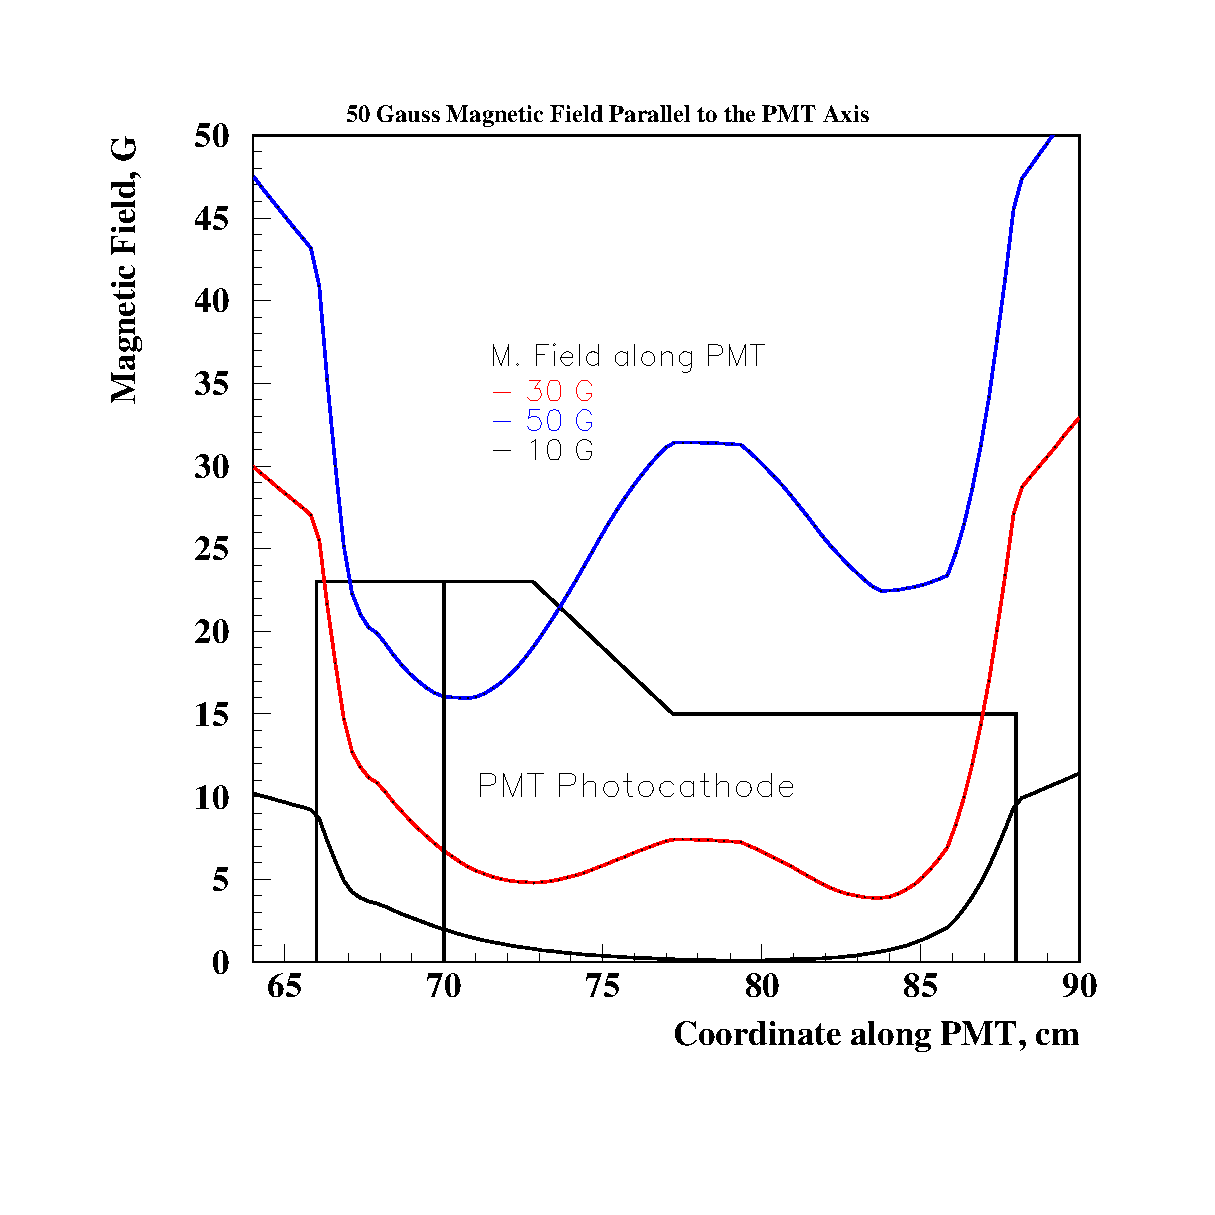
\includegraphics[height=7.5cm]{Magnetic-shielding/shield_z_lin.eps}
\vspace{0.5cm}
\caption{\small{Standard single-layer PMT magnetic shielding (shown in black).
The applied magnetic field is along the PMT axis: 50~G is shown in blue, 
40~G in red, and 30~G in black.  The PMT photocathode position is shown by 
the black the vertical line.}}
\label{lin_z}
\end{centering}
\end{figure}
%%%%%%%%%%%%%%%%%%%%%%%%%%%%%%%%%%%%%%%%%%%%%%%%%%%%%%%%%%%%%%%%%%%%%%%%

%%%%%%%%%%%%%%%%%%%%%%%%%%%%%%%%%%%%%%%%%%%%%%%%%%%%%%%%%%%%%%%%%%%%%%%%
\begin{figure}
\hspace{0.5cm}
\begin{centering}
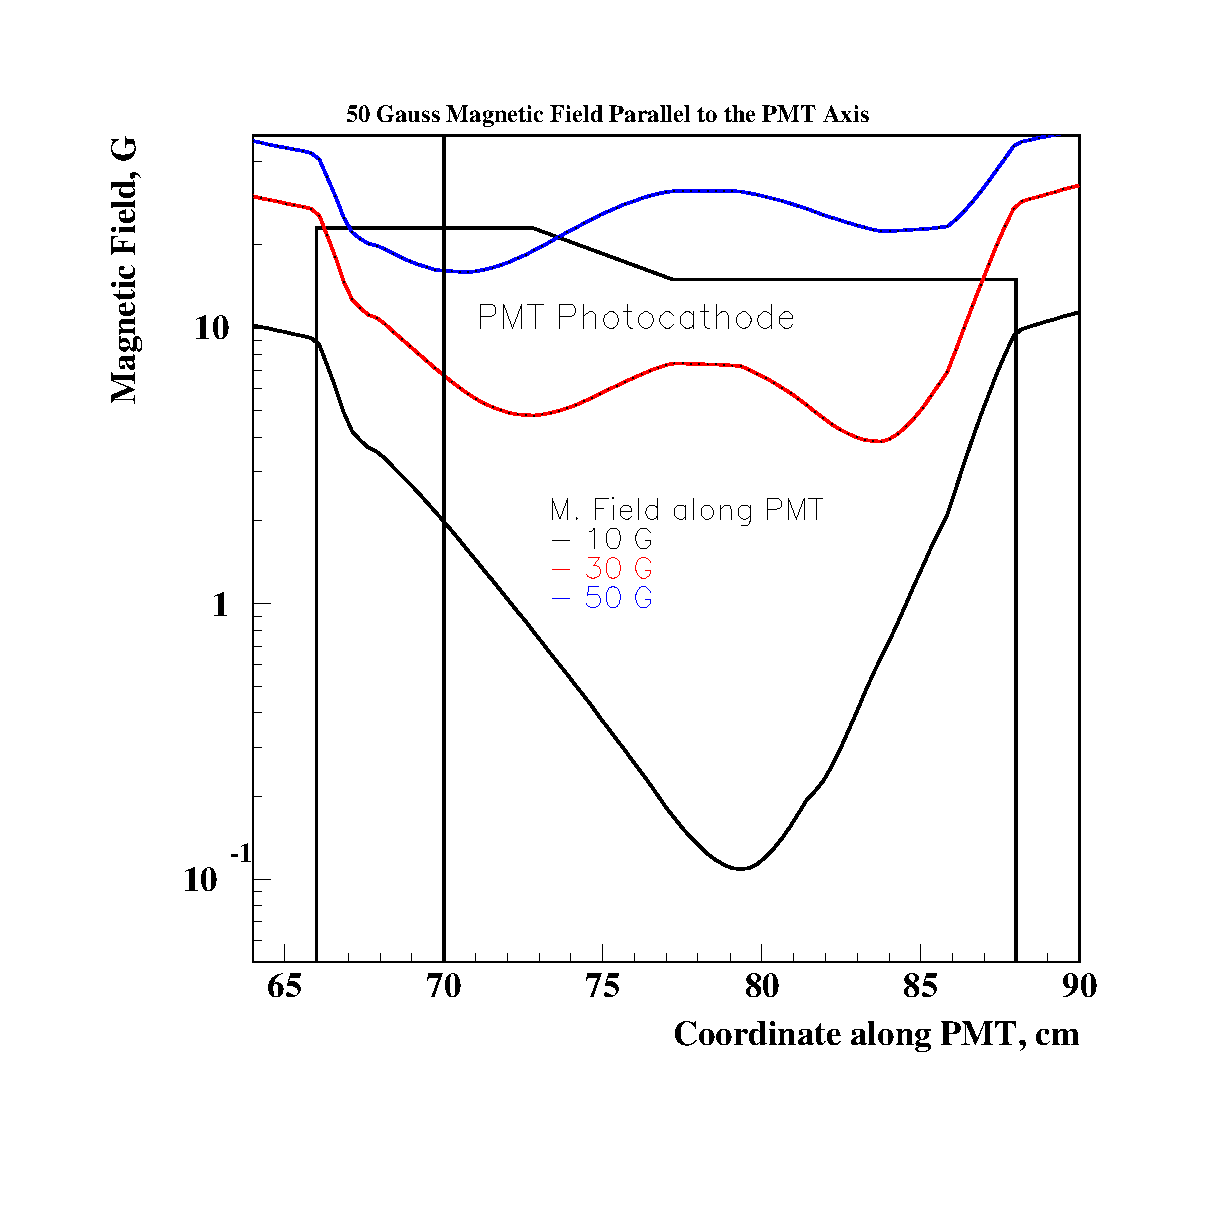
\includegraphics[height=7.5cm]{Magnetic-shielding/shield_z_log.eps}
\vspace{0.5cm}
\caption{\small{Same as Fig.~\ref{lin_z} but with a logarithmic $y$-axis.}}
\label{log_z}
\end{centering}
\end{figure}
%%%%%%%%%%%%%%%%%%%%%%%%%%%%%%%%%%%%%%%%%%%%%%%%%%%%%%%%%%%%%%%%%%%%%%%%

%%%%%%%%%%%%%%%%%%%%%%%%%%%%%%%%%%%%%%%%%%%%%%%%%%%%%%%%%%%%%%%%%%%%%%%%
\begin{figure}
\hspace{0.5cm}
\begin{centering}
\includegraphics[height=7.5cm]{Magnetic-shielding/3layers.eps}
\vspace{0.5cm}
\caption{\small{The effect of cylindrical PMT magnetic shielding, in which
the applied magnetic field is 20~G along the PMT axis. Single-layer shielding 
is shown in black, two-layer shielding is shown in red, and three-layer
shielding is shown in blue.  The PMT photocathode position is shown by 
the black vertical line.}}
\label{3layers}
\end{centering}
\end{figure}
%%%%%%%%%%%%%%%%%%%%%%%%%%%%%%%%%%%%%%%%%%%%%%%%%%%%%%%%%%%%%%%%%%%%%%%%

\subsection{Magnetic Shielding Test Stand}

A test stand (Fig.~\ref{magstand}) was used to study the magnetic 
shielding properties.  The magnetic shielding was placed inside a black 
box that is located between two circular magnetic coils that produce an 
external magnetic field.  A high-current power supply allows us to vary 
the current up to 107~A, which corresponds to a magnetic field value of 
68~G.  The calibration line showing the relation between current and the 
magnetic field is shown in Fig.~\ref{magcalibration}.  We have measured 
the magnetic field along the PMT axis inside the shielding by using the 
Gauss/Teslameter (Model 5070) measuring device. The results of the 
measurements for the single shielding layers are shown in 
Fig.~\ref{magshield1}.  Note that the first shielding layer is a prototype 
shield that was ordered for testing from the manufacturer.  It is a 
cylindrical magnetic shield, 50\% alloy of NiFe with a 6.19-in outer 
diameter, 6.06-in inner diameter, and 18.7-in long.  The second shield layer 
is a standard PMT magnetic shield.  Fig.~\ref{prototype-shielding} shows a 
drawing of the PMT and Winston Cone inserted inside the prototype shield. 
Results of the measurements for the double-layer shielding are shown in 
Fig.~\ref{magshield2}.  According to Fig.~\ref{magshield2}, we expect a
0.3~G magnetic field on the PMTs with the two-layer shield in a nominal 
30~G external magnetic field.  Studies of the PMT performance affected 
by different magnetic field conditions are underway.

%%%%%%%%%%%%%%%%%%%%%%%%%%%%%%%%%%%%%%%%%%%%%%%%%%%%%%%%%%%%%%%%%%%%%%%%
\begin{figure}
\hspace{0.5cm}
\begin{centering}
\includegraphics[height=7.5cm]{Magnetic-shielding/mag_stand.eps}
\vspace{0.5cm}
\caption{\small{Photograph of the magnetic shielding test stand.  The 
black box that contains the test shielding is located between the 
magnetic coils.}}
\label{magstand}
\end{centering}
\end{figure}
%%%%%%%%%%%%%%%%%%%%%%%%%%%%%%%%%%%%%%%%%%%%%%%%%%%%%%%%%%%%%%%%%%%%%%%%

%%%%%%%%%%%%%%%%%%%%%%%%%%%%%%%%%%%%%%%%%%%%%%%%%%%%%%%%%%%%%%%%%%%%%%%%
 \begin{figure}
 \hspace{0.5cm}
 \begin{centering}
  \includegraphics[height=7.5cm]{Magnetic-shielding/mag_calibration.eps}
 \vspace{0.5cm}
 \caption{\small{The current to magnetic field value calibration curve.}}
\label{magcalibration}
\end{centering}
 \end{figure}
%%%%%%%%%%%%%%%%%%%%%%%%%%%%%%%%%%%%%%%%%%%%%%%%%%%%%%%%%%%%%%%%%%%%%%%%

%%%%%%%%%%%%%%%%%%%%%%%%%%%%%%%%%%%%%%%%%%%%%%%%%%%%%%%%%%%%%%%%%%%%%%%%
 \begin{figure}
 \vspace{1.cm}
 \begin{centering}
  \includegraphics[height=7.5cm,angle=0]{Magnetic-shielding/magshield1.eps}
 \includegraphics[height=7.5cm,angle=0]{Magnetic-shielding/magshield2.eps}
 \hspace{0.1cm}
 \caption{\small{Results of the measurements of the magnetic field along 
the PMT axis inside the single-layer shield.  Left panel: The cylindrical 
shielding.  Right panel: The conventional PMT shielding.}}
\label{magshield1}
 \end{centering}
 \end{figure}
%%%%%%%%%%%%%%%%%%%%%%%%%%%%%%%%%%%%%%%%%%%%%%%%%%%%%%%%%%%%%%%%%%%%%%%%

%%%%%%%%%%%%%%%%%%%%%%%%%%%%%%%%%%%%%%%%%%%%%%%%%%%%%%%%%%%%%%%%%%%%%%%%
\begin{figure}
\hspace{0.5cm}
\begin{centering}
\includegraphics[height=10cm,angle=-90]{Magnetic-shielding/mag_shield.eps}
\vspace{0.5cm}
\caption{\small{Assembly of a photomultiplier tube with a Winston Cone 
magnetic shield.}}
\label{prototype-shielding}
\end{centering}
\end{figure}
%%%%%%%%%%%%%%%%%%%%%%%%%%%%%%%%%%%%%%%%%%%%%%%%%%%%%%%%%%%%%%%%%%%%%%%%

%%%%%%%%%%%%%%%%%%%%%%%%%%%%%%%%%%%%%%%%%%%%%%%%%%%%%%%%%%%%%%%%%%%%%%%%
 \begin{figure}
 \hspace{0.5cm}
 \begin{centering}
  \includegraphics[height=9.5cm]{Magnetic-shielding/magshield3.eps}
 \vspace{0.5cm}
 \caption{\small{Results of the measurements of the magnetic field along 
the PMT axis inside the double-layer shield combined from the two single 
layers shown in Fig.~\ref{magshield1}.}}  
\label{magshield2}
\end{centering}
 \end{figure}
%%%%%%%%%%%%%%%%%%%%%%%%%%%%%%%%%%%%%%%%%%%%%%%%%%%%%%%%%%%%%%%%%%%%%%%%

\subsection{PMT Laboratory Studies}

\subsubsection{Introduction}

Particles that pass through a medium with a higher velocity than the
phase velocity of light in that medium electromagnetically radiate
photons.  This is called {\v C}erenkov radiation.  The {\v C}erenkov 
photons are produced at an angle relative to the particle direction given by:

\begin{equation}
\cos\theta = \frac{1}{n\beta},
\end{equation}

\noindent
where $n$ is the index of refraction and $\beta=v/c$ is the particle 
velocity.

{\v C}erenkov detectors are usually used for particle identification.
Threshold {\v C}erenkov detectors make a yes/no decision based on whether 
the particle is above or below the threshold velocity $\beta_t=1/n$.
The more powerful use of {\v C}erenkov radiation comes from measuring the 
ring-correlated angles of emission of the {\v C}erenkov photons in a 
Ring Imaging {\v C}erenkov Counter (RICH).

The High Threshold {\v C}erenkov Counter for {\tt CLAS12} contains three 
main elements:

\begin{itemize}
\item a radiator through which the charged particle passes;
\item a mirror;
\item a photodetector.
\end {itemize} 

As  {\v C}erenkov radiation is a weak source of photons, light collection 
and photodetector efficiency must be as high as possible.

The number of photoelectrons ($N_{p.e.}$) per unit path length of a particle 
with charge $ze$ is:

\begin{equation}
\frac{dN_{p.e.}}{dx}=2\pi\alpha z^2\int{\frac {\epsilon(\lambda)}{\lambda^2}\displaystyle\left(1-\frac{1}{\beta^2n^2(\lambda)}\right)d\lambda},
\end{equation}

\noindent
where $x$ is the path length, $\epsilon(\lambda)$ is the efficiency for 
collecting the {\v C}erenkov light and transducing it into photoelectrons,
and $n(\lambda)$ is the index of refraction of the radiator, which is a 
function of photon energy or photon wavelength $\lambda$.  The typical 
energy-dependent variation of the index of refraction is modest, so we can 
write

\begin{equation}
\frac{dN_{p.e.}}{dx} = 2\pi\alpha z^2\displaystyle\left(1-\frac{1}{\beta^2n^2}\right)\int{\frac {\epsilon(\lambda)}{\lambda^2}d\lambda}.
\end{equation}

\noindent
The {\v C}erenkov detector quality factor (figure of merit) $N_0$ is defined 
as:

\begin{equation}
N_0 = 2\pi\alpha z^2\int{\frac {\epsilon(\lambda)}{\lambda^2}d\lambda},
\end{equation}

\noindent
So that

\begin{equation}
N_{p.e.}\approx L N_0 <sin^2\theta>,
\end{equation}

\noindent
where $L$ is the radiator length.

Careful designs of the {\v C}erenkov counter give values of $N_0$ for a 
PMT detection system working in the visible and near UV, that collect 
most of the {\v C}erenkov light of about 100~cm$^{-1}$.

The overall efficiency and rejection factors of the {\v C}erenkov counters 
are controlled by Poisson fluctuations, which can be especially critical for 
the separation of species where one particle type is dominant.  The 
effective number of photoelectrons is often less than the average number 
calculated above due to additional noise from the photodetector.  So, it is 
extremely important to design the detector with as high an average number of 
photoelectrons as possible.

The number of detected photoelectrons ($N_{p.e.}$), which is directly 
connected with the efficiency for collecting the {\v C}erenkov light and 
transducing it in photoelectrons $\epsilon(\lambda)$, contains several 
components:

\begin{equation}
\epsilon(\lambda) = \epsilon_{gas}(\lambda)\times\epsilon_{mirror}(\lambda)\times\epsilon_{PMT}(\lambda),
\end{equation}

\noindent
where $\epsilon_{gas}(\lambda)$ is the gas transparecy,
$\epsilon_{mirror}(\lambda)$ is the mirror reflectivity, and
$\epsilon_{PMT}(\lambda)$ is the PMT quantum efficiency.

One of the ways to increase the figure of merit $N_0$ is to use a PMT with 
a quartz input window.  The intensity of the photons produced in 
{\v C}erenkov radiation varies as $dN/d\lambda\sim1/\lambda^2$.  Therefore, 
it is critical to use PMTs that are efficient at low wavelengths where most 
of the light is produced.  The wavelength cutoff for a quartz PMT is in the 
region from 160--180~nm, in comparison with the 220--240~nm range for the 
UV glass PMT.  However, the quartz PMTs are more expensive.
 
\subsubsection{{\v C}erenkov Light Detection}
\label{sec:Cerenkov-Light-Detection}

The High Threshold {\v C}erenkov Counter (HTCC) for {\tt CLAS12} will 
contain a total of 48 mirrors and 48 PMTs.  The shape of the mirrors
and distribution of the PMTs for one sector of the detector is illustrated
in Fig.~\ref{HTCC_design}.  Two different types of PMTs were considered for 
the {\v C}erenkov Counters: the Photonis XP4508 quartz-faced PMT and the 
XP4500 UV glass-faced PMT.  Both models have uniform electron collection 
over their bialkali photocathodes and measure 5~in in diameter.  However, 
as seen in Fig.~\ref{quanteff_absorb}, the quartz PMTs are expected to have 
better quantum efficiency at low wavelengths than the UV glass PMTs. With 
increased efficiency, the quartz PMT should be able to detect more photons 
at higher energies than standard UV glass PMTs.
 
To study the performance of PMTs, a cosmic ray stand was used, which is 
described in Section~\ref{cosmicstand}.  In addition to studies of light 
collection by two different PMT types, we also measured the impact on light 
collection from different gas environments.  We used air and nitrogen.
Note that the HTCC will use CO$_2$ gas, but we will neglect the difference 
between CO$_2$ and nitrogen gas in our tests.  Nitrogen gas absorbs less 
light than air at low wavelengths.  The absorption factor of a gas, detailed 
in Fig.~\ref{quanteff_absorb}, is the fraction of light that the gas will 
allow to pass through it.  PMTs in a nitrogen gas environment should be able 
to detect more {\v C}erenkov light than those in air due to this improved 
transparency at low wavelengths. 

%%%%%%%%%%%%%%%%%%%%%%%%%%%%%%%%%%%%%%%%%%%%%%%%%%%%%%%%%%%%%%%%%%%%%%%
\begin{figure}
\hspace{0.5cm}
\begin{centering}
\includegraphics[height=9.0cm]{PMT-studies/vpk_2.eps}
\vspace{0.5cm}
\caption{\small{The current optical design for one sector of the HTCC. 
Eight PMTs will collect the {\v C}erenkov light reflected off of four 
mirrors.}}
\label{HTCC_design}
\end{centering}
\end{figure}
%%%%%%%%%%%%%%%%%%%%%%%%%%%%%%%%%%%%%%%%%%%%%%%%%%%%%%%%%%%%%%%%%%%%%%%

%%%%%%%%%%%%%%%%%%%%%%%%%%%%%%%%%%%%%%%%%%%%%%%%%%%%%%%%%%%%%%%%%%%%%%%
\begin{figure}
\vspace{0.5cm}
\begin{centering}
\includegraphics[height=6.0cm]{PMT-studies/pmt_2.eps}
\includegraphics[height=6.0cm]{PMT-studies/pmt_1.eps}
\vspace{0.5cm}
\caption{\small{Left: The quantum efficiency as a function of wavelength 
of the two Photonis PMT models being tested. Right: The absorption factors 
of nitrogen gas and air as a function of wavelength.}}
\label{quanteff_absorb}
\end{centering}
\end{figure}
%%%%%%%%%%%%%%%%%%%%%%%%%%%%%%%%%%%%%%%%%%%%%%%%%%%%%%%%%%%%%%%%%%%%%%%

Multiplying the gas absorption factor by the PMT quantum efficiency
and the $1/\lambda^2$ {\v C}erenkov light production dependence
gives, to a constant factor, the amount of {\v C}erenkov light collected
as a function of wavelength. The predicted amounts of light collected
for different gas and PMT-face configurations are plotted in 
Fig.~\ref{light_comparison}.  Taking the ratio of their integrals
for quartz and UV-glass in air gives:

\begin{equation}
\label{eq:light_ratio}
\frac{\textrm{Light}_{Quartz,\textrm{ }Air}}
{\textrm{Light}_{UV-Glass,\textrm{ }Air}} = 
\frac{\int_{0}^{\infty}QE_{Quartz}(\lambda)*AF_{Air}(\lambda)/\lambda^2d\lambda}
{\int_{0}^{\infty}QE_{UV-Glass}(\lambda)*AF_{Air}(\lambda)/\lambda^2\lambda}
= 1.2,
\end{equation}

\noindent
yielding a predicted 20\% improvement in light collection. Similarly,
in a nitrogen gas environment, this improvement increases to 25\%.
However, comparing the air and nitrogen gas environments for the quartz-faced
PMTs only results in a 4.5\% predicted increase in light collection.
The UV glass-faced PMT is predicted to achieve no appreciable improvement
in light collection in a nitrogen gas. This is because the quantum
efficiency of the XP4500 rapidly approaches zero for light with 
$\lambda < 200$~nm, the region where nitrogen gas has the most improvement 
over air.  These predictions are only preliminary, rough estimates as the
quantum efficiency measurements of the PMTs supplied by the manufacturer
are only characteristic approximations. 

%%%%%%%%%%%%%%%%%%%%%%%%%%%%%%%%%%%%%%%%%%%%%%%%%%%%%%%%%%%%%%%%%%%%%%%
\begin{figure}
\vspace{0.5cm}
\begin{centering}
\includegraphics[height=5.5cm]{PMT-studies/pmt_6.eps}
\includegraphics[height=5.5cm]{PMT-studies/pmt_5.eps}
\includegraphics[height=5.5cm]{PMT-studies/pmt_3.eps}
\includegraphics[height=5.5cm]{PMT-studies/pmt_4.eps}
\vspace{0.5cm}
\caption{\small{To a constant factor, the predicted amount of light collected 
as a function of wavelength for different PMT face and gas configurations,
plotted against each other for comparison.}}
\label{light_comparison}
\end{centering}
\end{figure}
%%%%%%%%%%%%%%%%%%%%%%%%%%%%%%%%%%%%%%%%%%%%%%%%%%%%%%%%%%%%%%%%%%%%%%%

\subsubsection{Cosmic Ray Stand}
\label{cosmicstand}

The predicted increase of detected photoelectrons in quartz-faced
PMTs is significant, so a test stand (see Fig.~\ref{test_stand})
was constructed to determine whether this performance increase is
reproducible.  A stack of 32 quartz plates was used as a medium for
{\v C}erenkov light generation as cosmic muons passed through them.
As diagrammed in Fig.~\ref{test_stand}, the {\v C}erenkov light was 
produced at a 46.7$^\circ$ angle from the incoming cosmic rays and was 
internally reflected until passing out of the end of the quartz plate. In 
a light-tight and air-tight box, the {\v C}erenkov radiation emitted by 
these cosmic rays was collected by two PMTs located an average of 11~cm 
away from the quartz plates.  While one of the PMTs was being tested, a 
second PMT was used as a reference to confirm the consistency of the 
experiment from test to test.  Three Photonis XP4508 quartz-faced PMTs and 
three Photonis XP4500 UV glass-faced PMTs were tested in air, and one of 
each type in nitrogen gas, which is close in optical properties to CO$_2$, 
which will be used in the HTCC.  A flow meter and pressure gauge were used 
to regulate the supply of nitrogen gas to the chamber during the final tests. 

%%%%%%%%%%%%%%%%%%%%%%%%%%%%%%%%%%%%%%%%%%%%%%%%%%%%%%%%%%%%%%%%%%%%%%%
\begin{figure}
\vspace{0.5cm}\begin{centering}
\includegraphics[height=5.0cm]{PMT-studies/IMG_0196.eps}
\includegraphics[height=5.0cm]{PMT-studies/cc_test.eps}
\vspace{0.5cm}
\caption{\small{A photograph (left) and schematic (right) of the cosmic 
ray stand used for testing the {\v C}erenkov light collection of different 
PMTs.  Trigger counters above and below the chamber detect a signal when 
a cosmic ray has passed through the quartz plates, and the two PMTs collect
the resulting {\v C}erenkov radiation. A flow meter and pressure gauge
are used to supply and regulate nitrogen gas to the chamber.}}
\label{test_stand}
\end{centering}
\end{figure}
%%%%%%%%%%%%%%%%%%%%%%%%%%%%%%%%%%%%%%%%%%%%%%%%%%%%%%%%%%%%%%%%%%%%%%%

To collect data, small scintillators attached to PMTs above and below
the test chamber were used to trigger event recording. A coincidence
between both PMTs indicated that a cosmic ray had passed through the
quartz plates, producing {\v C}erenkov light.  The trigger and data
acquisition systems are pictured and diagrammed in Fig.~\ref{trig_daq}.
The pulse height of the electrical signals from the PMT dynodes were
converted to digital ADCs for analysis. The ADC spectra of the two
trigger counters and the two {\v C}erenkov counters for one test run
are shown in Fig.~\ref{sample_adc}.  Cuts were placed around the peaks 
of the ADC spectra of the trigger PMTs to remove background events.  Also, 
the high voltage supplied to the PMTs was fixed throughout the experiment 
to make sure that the response of each of the PMTs was consistent. 

%%%%%%%%%%%%%%%%%%%%%%%%%%%%%%%%%%%%%%%%%%%%%%%%%%%%%%%%%%%%%%%%%%%%%%%
\begin{figure}
\vspace{0.5cm}\begin{centering}
\includegraphics[height=5.0cm]{PMT-studies/cerenk-daq.eps}
\includegraphics[height=5.0cm]{PMT-studies/daq.eps}
\vspace{0.5cm}
\caption{\small{Left: Data acquisition hardware. Right: Diagram of the 
triggering and DAQ process.}}
\label{trig_daq}
\end{centering}
\end{figure}
%%%%%%%%%%%%%%%%%%%%%%%%%%%%%%%%%%%%%%%%%%%%%%%%%%%%%%%%%%%%%%%%%%%%%%%

%%%%%%%%%%%%%%%%%%%%%%%%%%%%%%%%%%%%%%%%%%%%%%%%%%%%%%%%%%%%%%%%%%%%%%%
\begin{figure}
\vspace{0.5cm}\begin{centering}
\includegraphics[height=5.0cm]{PMT-studies/triggers.eps}
\includegraphics[height=5.0cm]{PMT-studies/cerenk_counters.eps}
\vspace{0.5cm}
\caption{\small{ADC spectra of the two trigger counters (top) and two 
{\v C}erenkov counters (bottom) for one test run.}}
\label{sample_adc}
\end{centering}
\end{figure}
%%%%%%%%%%%%%%%%%%%%%%%%%%%%%%%%%%%%%%%%%%%%%%%%%%%%%%%%%%%%%%%%%%%%%%%

\subsubsection{Calibration of the ADC Scale}

The ADC spectra of the test PMTs must be converted into units of collected
number of photoelectrons ($N_{p.e.}$) to judge PMT performance.  This 
conversion is linear because the multi-stage signal amplification process 
of the PMTs is independent of the number of photons detected.  The ADC
conversion factor for each PMT was found by using an LED to fix the
source intensity.  The LED and test PMTs were placed in a light-tight
box for testing.  Multiple tests were performed for each PMT, each
with a different intensity of LED source photons. 

The energy response of a PMT to a fixed intensity source of photons
is described by a Poisson-like distribution, 

\begin{equation}
N(ADC) = \frac{N_{0}\mu^{\frac{ADC}{\mu_1}}e^{-\mu}}{\mu_{1}
\Gamma(\frac{ADC}{\mu_1}+1)},\textrm{ }\Gamma(x)=\int_0^\infty t^{x-1}e^{-t}dt,
\end{equation}

\noindent
where $\mu$ is the average number of photoelectrons, $\mu_1$ is
the ADC to $N_{p.e.}$ conversion factor, and $N_0$ is the scaling factor.
The Poisson distribution fits to the ADC spectra of different light
intensities for the three UV-glass-faced PMTs and the three quartz-faced
PMTs are shown in Figs.~\ref{poisson_uvglass} and \ref{poisson_quartz},
respectively. To find the average conversion factor, the average ADC
vs. the average $N_{p.e.}$ were plotted in Figs.~\ref{linear_uvglass}
and \ref{linear_quartz} and fit to a linear function.  The slope
of these fits gives the ADC to $N_{p.e.}$ conversion factor for each 
test PMT. 

%%%%%%%%%%%%%%%%%%%%%%%%%%%%%%%%%%%%%%%%%%%%%%%%%%%%%%%%%%%%%%%%%%%%%%%
\begin{figure}
\vspace{0.5cm}
\begin{centering}
\includegraphics[height=10.0cm]{PMT-studies/uv_9700_v1_fits.eps}
\end{centering}
\begin{centering}
\includegraphics[height=9.5cm]{PMT-studies/uv_9705_v1_fits.eps}
\includegraphics[height=9.5cm]{PMT-studies/uv_9719_v1_fits.eps}
\vspace{0.5cm}
\caption{\small{Poisson fits to ADC spectra of the three UV glass-faced 
PMTs.  Here, $P1$ is the ADC to $N_{p.e.}$ conversion factor $\mu_1$, and 
$P2$ is the average number of photoelectrons, $\mu$.}}
\label{poisson_uvglass}
\end{centering}
\end{figure}
%%%%%%%%%%%%%%%%%%%%%%%%%%%%%%%%%%%%%%%%%%%%%%%%%%%%%%%%%%%%%%%%%%%%%%%

%%%%%%%%%%%%%%%%%%%%%%%%%%%%%%%%%%%%%%%%%%%%%%%%%%%%%%%%%%%%%%%%%%%%%%%
\begin{figure}
\vspace{0.5cm}
\begin{centering}
\includegraphics[height=10.0cm]{PMT-studies/qt_0100_v2_fits.eps}
\end{centering}
\begin{centering}
\includegraphics[height=9.5cm]{PMT-studies/qt_0102_v1_fits.eps}
\includegraphics[height=9.5cm]{PMT-studies/qt_0103_v1_fits.eps}
\vspace{0.5cm}
\caption{\small{Poisson fits to ADC spectra of the three quartz-faced 
PMTs.  Here, $P1$ is the ADC to $N_{p.e.}$ conversion factor $\mu_1$, 
and $P2$ is the average number of photoelectrons, $\mu$.}}
\label{poisson_quartz}
\end{centering}
\end{figure}
%%%%%%%%%%%%%%%%%%%%%%%%%%%%%%%%%%%%%%%%%%%%%%%%%%%%%%%%%%%%%%%%%%%%%%%

%%%%%%%%%%%%%%%%%%%%%%%%%%%%%%%%%%%%%%%%%%%%%%%%%%%%%%%%%%%%%%%%%%%%%%%
\begin{figure}
\vspace{0.5cm}
\begin{centering}
\includegraphics[height=8.5cm]{PMT-studies/uv_9700_v1_result.eps}
\end{centering}
\begin{centering}
\includegraphics[height=8.0cm]{PMT-studies/uv_9705_v1_result.eps}
\includegraphics[height=8.0cm]{PMT-studies/uv_9719_v1_result.eps}
\vspace{0.5cm}
\caption{\small{Linear fits to the average ADC value vs. the average 
$N_{p.e.}$ of the Poisson distributions of the three UV glass-faced PMTs. 
The slopes are the ADC to $N_{p.e.}$ conversion factors.}}
\label{linear_uvglass}
\end{centering}
\end{figure}
%%%%%%%%%%%%%%%%%%%%%%%%%%%%%%%%%%%%%%%%%%%%%%%%%%%%%%%%%%%%%%%%%%%%%%%

%%%%%%%%%%%%%%%%%%%%%%%%%%%%%%%%%%%%%%%%%%%%%%%%%%%%%%%%%%%%%%%%%%%%%%%
\begin{figure}
\vspace{0.5cm}
\begin{centering}
\includegraphics[height=8.5cm]{PMT-studies/qt_0100_v2_result.eps}
\end{centering}
\begin{centering}
\includegraphics[height=8.0cm]{PMT-studies/qt_0102_v1_result.eps}
\includegraphics[height=8.0cm]{PMT-studies/qt_0103_v1_result.eps}
\vspace{0.5cm}
\caption{\small{Linear fits to the average ADC value vs. the average 
$N_{p.e.}$ of the Poisson distributions of the three quartz-faced PMTs.  
The slopes are the ADC to $N_{p.e.}$ conversion factors.}}
\label{linear_quartz}
\end{centering}
\end{figure}
%%%%%%%%%%%%%%%%%%%%%%%%%%%%%%%%%%%%%%%%%%%%%%%%%%%%%%%%%%%%%%%%%%%%%%%

To check that these conversion factors were correct, each PMT was tested
with the LED emitting only a single photon.  As seen in 
Fig.~\ref{numphe_check}, the conversion factors were applied to the ADC 
spectra and the mean number of photoelectrons for each distribution was 
approximately one, indicating that the conversion factors are correct. 

%%%%%%%%%%%%%%%%%%%%%%%%%%%%%%%%%%%%%%%%%%%%%%%%%%%%%%%%%%%%%%%%%%%%%%%
\begin{figure}
\hspace{0.5cm}
\begin{centering}
\includegraphics[height=10.5cm]{PMT-studies/al_phe.eps}
\vspace{0.5cm}
\caption{\small{$N_{p.e.}$ spectra for a single-photon LED source for 
the six test PMTs.  The means of each distribution are all near one, 
indicating that the ADC to $N_{p.e.}$ conversion factors are correct.}}
\label{numphe_check}
\end{centering}
\end{figure}
%%%%%%%%%%%%%%%%%%%%%%%%%%%%%%%%%%%%%%%%%%%%%%%%%%%%%%%%%%%%%%%%%%%%%%%

\subsubsection{{\v C}erenkov Light Test Results}

Using the ADC to $N_{p.e.}$ conversion factors, the three Photonis XP4508
quartz- and three Photonis XP4500 UV glass-faced PMTs were tested with 
the cosmic ray stand filled with air.  The results of the tests, with each
measured for about a week, are shown in Fig.~\ref{numphe_all}, which
highlights the $N_{p.e.}$ spectra from collecting the {\v C}erenkov
radiation.  Fig.~\ref{avg_numphe} illustrates the average $N_{p.e.}$ for 
each PMT-face type, yielding an increase of $45 \pm 4$\% in the number of 
detected {\v C}erenkov photoelectrons in quartz-faced PMTs over UV 
glass-faced PMTs.  This result is larger than the predicted increase of 20\% 
found in eq.(\ref{eq:light_ratio}).  This difference is most likely due to 
an error in the rough quantum efficiency estimate that the manufacturer 
supplied.  Fig.~\ref{ref_pmt} shows a fit to the average number of 
photoelectrons collected by the quartz reference PMT throughout the two 
months of testing.  In five tests, the maximum deviation from the average of 
58 photoelectrons was 4.1\%, which may be considered as an estimate of the 
systematic uncertainty of the experiment. 

%%%%%%%%%%%%%%%%%%%%%%%%%%%%%%%%%%%%%%%%%%%%%%%%%%%%%%%%%%%%%%%%%%%%%%%
\begin{figure}
\hspace{0.5cm}
\begin{centering}
\includegraphics[height=10.5cm]{PMT-studies/all_phe_spectra.eps}
\vspace{0.5cm}
\caption{\small{$N_{p.e.}$ spectra from collecting {\v C}erenkov light in 
the cosmic ray stand for the three UV glass- and three quartz-faced PMTs.}}
\label{numphe_all}
\end{centering}
\end{figure}
%%%%%%%%%%%%%%%%%%%%%%%%%%%%%%%%%%%%%%%%%%%%%%%%%%%%%%%%%%%%%%%%%%%%%%%

%%%%%%%%%%%%%%%%%%%%%%%%%%%%%%%%%%%%%%%%%%%%%%%%%%%%%%%%%%%%%%%%%%%%%%%
\begin{figure}
\hspace{0.5cm}
\begin{centering}
\includegraphics[height=7.5cm]{PMT-studies/uv.eps}
\includegraphics[height=7.5cm]{PMT-studies/qt.eps}
\vspace{0.5cm}
\caption{\small{Fits to find the average $N_{p.e.}$ for UV glass- and 
quartz-faced PMTs.}}
\label{avg_numphe}
\end{centering}
\end{figure}
%%%%%%%%%%%%%%%%%%%%%%%%%%%%%%%%%%%%%%%%%%%%%%%%%%%%%%%%%%%%%%%%%%%%%%%

%%%%%%%%%%%%%%%%%%%%%%%%%%%%%%%%%%%%%%%%%%%%%%%%%%%%%%%%%%%%%%%%%%%%%%%
\begin{figure}
\hspace{0.5cm}
\begin{centering}
\includegraphics[height=9.5cm]{PMT-studies/stab.eps}
\vspace{0.5cm}
\caption{\small{The number of photoelectrons collected by the reference 
PMT during testing.  The maximum deviation of 4.1\% is a reflection of 
the systematic uncertainty of the experiment.}}
\label{ref_pmt}
\end{centering}
 \end{figure}
%%%%%%%%%%%%%%%%%%%%%%%%%%%%%%%%%%%%%%%%%%%%%%%%%%%%%%%%%%%%%%%%%%%%%%%

%%%%%%%%%%%%%%%%%%%%%%%%%%%%%%%%%%%%%%%%%%%%%%%%%%%%%%%%%%%%%%%%%%%%%%%
\begin{figure}
\hspace{0.5cm}
\begin{centering}
\includegraphics[height=9.5cm]{PMT-studies/gas_spectra.eps}
\vspace{0.5cm}
\caption{\small{$N_{p.e.}$ spectra for UV-glass and quartz-faced PMTs in 
a nitrogen gas environment.}}
\label{ntogas}
\end{centering}
\end{figure}
%%%%%%%%%%%%%%%%%%%%%%%%%%%%%%%%%%%%%%%%%%%%%%%%%%%%%%%%%%%%%%%%%%%%%%%

%%%%%%%%%%%%%%%%%%%%%%%%%%%%%%%%%%%%%%%%%%%%%%%%%%%%%%%%%%%%%%%%%%%%%%%
\begin{figure}
\hspace{0.5cm}
\begin{centering}
\includegraphics[height=9.5cm]{PMT-studies/gas.eps}
\vspace{0.5cm}
\caption{\small{Ratio of light collection in nitrogen gas to the air 
environment for UV-glass and quartz`faced PMTs.}}
\label{gas}
\end{centering}
\end{figure}
%%%%%%%%%%%%%%%%%%%%%%%%%%%%%%%%%%%%%%%%%%%%%%%%%%%%%%%%%%%%%%%%%%%%%%%

One quartz- and one UV glass-faced PMT were tested in the cosmic ray
stand with the chamber filled with nitrogen gas.  Fig.~\ref{ntogas}
illustrates the $N_{p.e.}$ spectra for these tests, yielding an average
photoelectron detection increase of 82\%.  This is much larger than
the predicted increase of 25\% from Section~\ref{sec:Cerenkov-Light-Detection}.
As mentioned previously, the rough quantum efficiency distributions
supplied by Photonis are likely incorrect.  Additionally, only one PMT 
of each type was tested; thus this difference may be inflated by the 
inconsistent response between PMTs of the same model.  So, this estimate 
based on a single measurement is very crude.  The amount of light collected 
by the quartz-faced PMT in a nitrogen gas environment was 7\% more than in 
air, similar to the predicted increase of 4.5\% from
Section~\ref{sec:Cerenkov-Light-Detection}.  The amount of light collected 
by the UV glass-faced PMT actually decreased by 2\% in nitrogen gas, as 
opposed to the negligible difference that was predicted (see Fig.~\ref{gas}). 

In summary, using a cosmic ray test stand, the Photonis XP4508 quartz-faced 
PMTs were found to collect 45\% more {\v C}erenkov radiated photoelectrons
in air than the Photonis XP4500 UV glass-faced PMTs.  In a nitrogen gas 
environment, the {\v C}erenkov light collection of the quartz-faced
PMTs improved by an additional 7\%, so the total gain is estimated  
to be 55\% ($1.45\times1.07$=1.55). 

\section{Mechanical Design}

The basic shape of the HTCC is naturally generated by a combination of 
the dimensions and positions of the surrounding equipment, certain 
required acceptance angles, and the planned focal points of the mirror 
within.  The body will serve primarily as a gas volume container, and 
should have as little material as possible within to obstruct either the 
{\v C}erenkov light, or particles to other detectors.  An overall view of 
the appearance of the HTCC is shown in Fig.~\ref{overall}.
 
%%%%%%%%%%%%%%%%%%%%%%%%%%%%%%%%%%%%%%%%%%%%%%%%%%%%%%%%%%%%%%%%%%%%%%%%%
\begin{figure}[h]
\vspace{0.5cm}
\begin{centering}
\includegraphics[height=9.0cm,angle=-0]{Mechanical/CD3_Cyril_1.eps}
\hspace{0.1cm}
\caption{\small{Overall appearance of the HTCC viewed from upstream side.}}
\label{overall}
\end{centering}
\end{figure}
%%%%%%%%%%%%%%%%%%%%%%%%%%%%%%%%%%%%%%%%%%%%%%%%%%%%%%%%%%%%%%%%%%%%%%%%%

\subsection{Main Structure}

The geometry of the detector strongly dictates the shape of the HTCC's main 
structure.  The mirror design is a twelve segment combined mirror, and the 
light is focused to twelve banks of 4 photomultiplier tubes per bank.  For 
this mirror, a twelve-sided shell centered around the beamline was designed, 
with space on each segment to mount one row of four PMTs. The shell was 
designed to completely enclose all of the PMTs, mounting hardware, shielding, 
etc..  The strength of the structure comes from the entry cone, the downstream 
mirror housing, and the connecting ribs of rectangular tubing.  The outer 
web of aluminum angles and tees will add to the strength of the unit, but 
is primarily to serve as a frame for panels used to seal the gas volume. The 
structure is still simple, and can be constructed of flat and rolled, 
machined and welded plates, tees, and/or angles of Aluminum (see 
Fig.~\ref{structure}).

%%%%%%%%%%%%%%%%%%%%%%%%%%%%%%%%%%%%%%%%%%%%%%%%%%%%%%%%%%%%%%%%%%%%%%%%%
\begin{figure}[h]
\vspace{0.5cm}
\begin{centering}
\includegraphics[height=9.0cm,angle=-90]{Mechanical/CD3_Cyril_2.eps}
\hspace{0.1cm}
\caption{\small{Mechanical housing of the HTCC.}}
\label{structure}
\end{centering}
\end{figure}
%%%%%%%%%%%%%%%%%%%%%%%%%%%%%%%%%%%%%%%%%%%%%%%%%%%%%%%%%%%%%%%%%%%%%%%%%

\subsection{PMT Mount}

Our original goal was to have the PMTs mounted to the outer surface of 
the HTCC to make maintenance easier, but finding an effective way to seal 
the gas volume, while maintaining some degree of adjustability at each PMT 
within the space available proved to be challenging.  Instead, each PMT, 
Light Concentrator, and any shielding is mounted to one bracket, as shown
in Fig.~\ref{bracket}.  The brackets are mounted to a plate (eight each) as
shown in Fig.~\ref{plate}, and the gas volume of the HTCC is sealed via 
access panels located radially beyond the PMTs as shown in Fig.~\ref{pannels}.
This system is relatively easier and less expensive to manufacture, easy to 
assemble, and each PMT is independently adjustable.

%%%%%%%%%%%%%%%%%%%%%%%%%%%%%%%%%%%%%%%%%%%%%%%%%%%%%%%%%%%%%%%%%%%%%%%%%
\begin{figure}[h]
\vspace{0.5cm}
\begin{centering}
\includegraphics[height=8.0cm,angle=-0]{Mechanical/CD3_Cyril_3.eps}
\hspace{0.1cm}
\caption{\small{Photomultiplier tube with Winston Light Concentrator, 
magnetic shield layers, and mounting block.}}
\label{bracket}
\end{centering}
\end{figure}
%%%%%%%%%%%%%%%%%%%%%%%%%%%%%%%%%%%%%%%%%%%%%%%%%%%%%%%%%%%%%%%%%%%%%%%%%

%%%%%%%%%%%%%%%%%%%%%%%%%%%%%%%%%%%%%%%%%%%%%%%%%%%%%%%%%%%%%%%%%%%%%%%%%
\begin{figure}[h]
\begin{centering}
\includegraphics[height=11.0cm,angle=-90]{Mechanical/CD3_Cyril_4.eps}
\hspace{0.1cm}
\caption{\small{Four photomultiplier tubes with Winston Light Concentrators 
and magnetic shield layers mounted to a plate.}}
\label{plate}
\end{centering}
\end{figure}
%%%%%%%%%%%%%%%%%%%%%%%%%%%%%%%%%%%%%%%%%%%%%%%%%%%%%%%%%%%%%%%%%%%%%%%%%

%%%%%%%%%%%%%%%%%%%%%%%%%%%%%%%%%%%%%%%%%%%%%%%%%%%%%%%%%%%%%%%%%%%%%%%%%
\begin{figure}[h]
\vspace{0.5cm}
\begin{centering}
\includegraphics[height=14cm,angle=-90]{Mechanical/CD3_Cyril_5.eps}
\hspace{0.1cm}
\caption{\small{Access panels covering identical banks of 4 PMTs.}}
\label{pannels}
\end{centering}
\end{figure}
%%%%%%%%%%%%%%%%%%%%%%%%%%%%%%%%%%%%%%%%%%%%%%%%%%%%%%%%%%%%%%%%%%%%%%%%%

\subsection{Mirror Positioning and Alignment}

Using six dual ball-socket adjustment linkages that contact the mirror in 
three places, the mirror can be securely supported and adjusted in all 
directions without inducing any torsional stress upon the mirror.  With 
this system (see Fig.~\ref{linkage}), the mirror would also be protected 
from possible stresses that the main shell may sustain, whether via 
temperature changes, transport, maintenance, or other unforeseen events. 

%%%%%%%%%%%%%%%%%%%%%%%%%%%%%%%%%%%%%%%%%%%%%%%%%%%%%%%%%%%%%%%%%%%%%%%%%
\begin{figure}[h]
\begin{centering}
\includegraphics[height=7.0cm,angle=-0]{Mechanical/CD_2_Cyril_6.eps}
\hspace{0.1cm}
\caption{\small{HTCC mirror supported in three places using adjustment 
linkages.}}
\label{linkage}
\end{centering}
\end{figure}
%%%%%%%%%%%%%%%%%%%%%%%%%%%%%%%%%%%%%%%%%%%%%%%%%%%%%%%%%%%%%%%%%%%%%%%%%

\subsection{Upstream and Entry}

The upstream end of the HTCC must wrap closely around the CTOF and 
solenoid magnet, to both avoid interfering with the light paths, and to 
allow for the greatest possible acceptance angle from the target. This 
results in a cup shape that reaches from the outside of the solenoid magnet, 
around the downstream CTOF light guides, with a cone in the center that 
follows the light guides back in toward the center of the solenoid, stopping 
just before the SVT.  This entry cone must be as thin as possible to retain 
every available degree of entry angle.  Currently, the optimized entry 
acceptance angle of 36$^\circ$ is limited by the solenoid shape and the 
position of the CTOF light guides.  This angle is only achievable using 
equipment clearances as low as 0.20~in, and an entry cone thickness of 
0.040~in.  At this thickness, the cone could be made of aluminum or a 
carbon composite; it is not a structural member, and only needs to be 
strong enough to support itself and the entry window.  A view of the entry 
structure is shown in Fig.~\ref{entry}.

%%%%%%%%%%%%%%%%%%%%%%%%%%%%%%%%%%%%%%%%%%%%%%%%%%%%%%%%%%%%%%%%%%%%%%%%%
\begin{figure}[h]
\begin{centering}
\includegraphics[height=16.0cm,angle=270]{Mechanical/CD3_Cyril_7.eps}
\hspace{0.1cm}
\caption{\small{HTCC mechanical entry structure.}}
\label{entry}
\end{centering}
\end{figure}
%%%%%%%%%%%%%%%%%%%%%%%%%%%%%%%%%%%%%%%%%%%%%%%%%%%%%%%%%%%%%%%%%%%%%%%%%

\subsection{Exit Scheme}

From the portion of the shell where the photomultiplier tubes are mounted, 
a cylindrical tube reaches downstream to house and support the mirror and 
adjustment fixtures, and finally interfaces with the exit window.  The 
exit window of the HTCC is located approximately 0.5~in past the mirror of 
the HTCC. It must allow up to 41$^\circ$ particles to pass through the gas 
volume unobstructed.  Because of the shape of the next detector in the 
beamline (Region~1 drift chamber), the outer edge of the HTCC exit window 
must be beveled to avoid interference with Region~1, see Fig.~\ref{exit}.

%%%%%%%%%%%%%%%%%%%%%%%%%%%%%%%%%%%%%%%%%%%%%%%%%%%%%%%%%%%%%%%%%%%%%%%%%
\begin{figure}[h]
\vspace{1cm}
\begin{centering}
\includegraphics[height=15.0cm,angle=-90]{Mechanical/CD3_Cyril_8.eps}
\hspace{0.1cm}
\vspace{1cm}
\caption{\small{View of the mechanical components of the outer shell.}} 
\label{exit}
\end{centering}
\end{figure}
%%%%%%%%%%%%%%%%%%%%%%%%%%%%%%%%%%%%%%%%%%%%%%%%%%%%%%%%%%%%%%%%%%%%%%%%%

 
\section{Cost estimates}
\label{Cost}

The following table summarizes estimated costs of expected procurement of items for HTCC and expenses on manufacturing related components. Costs for all procurement items were obtained from budgetary estimates provided by vendors upon official requests, or from catalogs when possible.
Expenses on construction were estimated either from most recent actual payments in FY06 for manufacturing of items very similar of those listed in table, or were based on engineering judgment and provided by vendor. 




\begin{table}
\centering
\caption{Cost for HTCC Construction}
\label{HTCC}
\vspace{0.5cm}
\begin{tabular}{|c|p{3.7cm}|c|c|p{1.4cm}|p{1.6cm}|p{1.5cm}|p{1.2cm}|p{2.5cm}|}
\hline
 & {\footnotesize\bf Item} & {\footnotesize\bf Un} & {\footnotesize\bf Amn} & {\footnotesize\bf Price, \$} & {\footnotesize\bf Source} & {\footnotesize\bf Cost, k\$}& {\footnotesize\bf Date} & {\footnotesize\bf Comments} \\ \hline

{\footnotesize 1} & {\footnotesize Winston Cone} & {\footnotesize EA} & {\footnotesize 96} & {\footnotesize 325.00} & {\footnotesize Budg Est} & {\footnotesize 38.70} & {\footnotesize 02.07.07} & {\footnotesize 7.5k set-up fee}\\ \hline

{\footnotesize 2} & {\footnotesize PMT XP4508, Quartz} & {\footnotesize EA} & {\footnotesize 96} & {\footnotesize 3256.00} & {\footnotesize Budg Est} & {\footnotesize 312.58} & {\footnotesize 05.09.07} & {\footnotesize }\\ \hline

{\footnotesize 3} & {\footnotesize HV divider VD105K} & {\footnotesize EA} & {\footnotesize 96} & {\footnotesize 152.00} & {\footnotesize Budg Est} & {\footnotesize 14.59} & {\footnotesize 05.09.07} & {\footnotesize }\\ \hline

{\footnotesize 4} & {\footnotesize Magnetic Shield} & {\footnotesize EA} & {\footnotesize 96} & {\footnotesize 402.15} & {\footnotesize Budg Est} & {\footnotesize 38.61} & {\footnotesize 03.16.07} & {\footnotesize }\\ \hline


{\footnotesize 5} & {\footnotesize Al+MgF$_{2}$ deposition} & {\footnotesize EA} & {\footnotesize 96} & {\footnotesize 177.08} & {\footnotesize Budg Est} & {\footnotesize 17.00} & {\footnotesize 03.09.07} & {\footnotesize }\\ \hline

{\footnotesize 6} & {\footnotesize HV Cable RG8X} & {\footnotesize ft} & {\footnotesize 9850} & {\footnotesize 0.60} & {\footnotesize Catalog} & {\footnotesize 5.91} & {\footnotesize 06.11.07} & {\footnotesize 2500V rated}\\ \hline

{\footnotesize 7} & {\footnotesize HV Connector PE-4193} & {\footnotesize EA} & {\footnotesize 100} & {\footnotesize 10.00} & {\footnotesize Catalog} & {\footnotesize 1.00} & {\footnotesize 06.11.07} & {\footnotesize Front Mount}\\ \hline

{\footnotesize 8} & {\footnotesize HV Connector PE-4493} & {\footnotesize EA} & {\footnotesize 192} & {\footnotesize 16.68} & {\footnotesize Catalog} & {\footnotesize 3.20} & {\footnotesize 06.11.07} & {\footnotesize For RG8X cable}\\ \hline

{\footnotesize 9} & {\footnotesize Signal Cable PE-B3199} & {\footnotesize ft} & {\footnotesize 25200} & {\footnotesize 0.63} & {\footnotesize Catalog} & {\footnotesize 15.90} & {\footnotesize 06.11.07} & {\footnotesize }\\ \hline

{\footnotesize 10} & {\footnotesize BNC Connector PE4386} & {\footnotesize EA} & {\footnotesize 192} & {\footnotesize 8.32} & {\footnotesize Catalog} & {\footnotesize 1.60} & {\footnotesize 06.11.07} & {\footnotesize For PE-B3199}\\ \hline

{\footnotesize 11} & {\footnotesize BNC Connector PE4014} & {\footnotesize EA} & {\footnotesize 100} & {\footnotesize 3.32} & {\footnotesize Catalog} & {\footnotesize 0.33} & {\footnotesize 06.11.07} & {\footnotesize Panel Mount}\\ \hline

{\footnotesize 12} & {\footnotesize Pump EW-07061-42} & {\footnotesize EA} & {\footnotesize 1} & {\footnotesize 398.00} & {\footnotesize Catalog} & {\footnotesize 0.40} & {\footnotesize 06.12.07} & {\footnotesize For Gas System}\\ \hline

{\footnotesize 13} & {\footnotesize Power Supply S-240-15} & {\footnotesize EA} & {\footnotesize 1} & {\footnotesize 93.48} & {\footnotesize Catalog} & {\footnotesize 0.1} & {\footnotesize 06.12.07} & {\footnotesize }\\ \hline

{\footnotesize 14} & {\footnotesize Controller 250E-4-D} & {\footnotesize EA} & {\footnotesize 1} & {\footnotesize 2496.00} & {\footnotesize Catalog} & {\footnotesize 2.50} & {\footnotesize 06.12.07} & {\footnotesize }\\ \hline


{\footnotesize 15} & {\footnotesize Transformer F-108U} & {\footnotesize EA} & {\footnotesize 1} & {\footnotesize 29.26} & {\footnotesize Catalog} & {\footnotesize 0.09} & {\footnotesize 06.12.07} & {\footnotesize }\\ \hline

{\footnotesize 16} & {\footnotesize Utl Chassis CHA-5X21} & {\footnotesize EA} & {\footnotesize 2} & {\footnotesize 133.51} & {\footnotesize Catalog} & {\footnotesize 0.27} & {\footnotesize 06.12.07} & {\footnotesize }\\ \hline

{\footnotesize 17} & {\footnotesize Controller DP25B-EAR} & {\footnotesize EA} & {\footnotesize 1} & {\footnotesize 395.00} & {\footnotesize Catalog} & {\footnotesize 0.40} & {\footnotesize 06.12.07} & {\footnotesize }\\ \hline

{\footnotesize 18} & {\footnotesize 1/2'' Stl Steel Tubing} & {\footnotesize ft} & {\footnotesize 400} & {\footnotesize 2.92(Sc)} & {\footnotesize Prev Proc} & {\footnotesize 1.17} & {\footnotesize 06.12.07} & {\footnotesize }\\ \hline

{\footnotesize 19} & {\footnotesize Cable 1255/8BK002} & {\footnotesize ft} & {\footnotesize 500} & {\footnotesize 1969.06} & {\footnotesize Catalog} & {\footnotesize 1.97} & {\footnotesize 06.12.07} & {\footnotesize Shielded}\\ \hline

{\footnotesize 20} & {\footnotesize Miscellaneous parts} & {\footnotesize } & {\footnotesize } & {\footnotesize } & {\footnotesize Eng Jdgm} & {\footnotesize 2.00} & {\footnotesize 06.12.07} & {\footnotesize }\\ \hline


\multicolumn{9}{|l|}{ \bf \hspace{0.5cm} Subtotal (procurement of components): \hspace{1.6cm} 458.32k }  \\ \hline


{\footnotesize 1} & {\footnotesize Mechanical Structure} & {\footnotesize HR} & {\footnotesize 700} & {\footnotesize 50.00} & {\footnotesize Eng Jdgm} & {\footnotesize 35.00} & {\footnotesize 04.02.07} & {\footnotesize }\\ \hline

{\footnotesize 2} & {\footnotesize Tooling Manufacturing} & {\footnotesize HR} & {\footnotesize 1008} & {\footnotesize 50.00} & {\footnotesize Budg Est} & {\footnotesize 50.40} & {\footnotesize 06.15.07} & {\footnotesize One set }\\ \hline

{\footnotesize 3} & {\footnotesize Substrates Manufactur.} & {\footnotesize HR} & {\footnotesize 2784} & {\footnotesize 50.00} & {\footnotesize Budg Est} & {\footnotesize 139.2} & {\footnotesize 06.15.07} & {\footnotesize Tot=96 substr}\\ \hline

{\footnotesize 4} & {\footnotesize Material, Al Profile} & {\footnotesize Lb} & {\footnotesize 5819} & {\footnotesize 6.00} & {\footnotesize Budg Est} & {\footnotesize 34.91} & {\footnotesize 04.03.07} & {\footnotesize For Mech Struct}\\ \hline

{\footnotesize 5} & {\footnotesize Rohacell foam HF31} & {\footnotesize EA} & {\footnotesize 1.5} & {\footnotesize 2800.00} & {\footnotesize Prev Proc} & {\footnotesize 4.20} & {\footnotesize 05.04.07} & {\footnotesize For 96 Substr.}\\ \hline

\multicolumn{9}{|l|}{ \bf \hspace{0.5cm} Subtotal (machine shop expenses): \hspace{2.6cm} 263.71k }  \\ \hline
\multicolumn{9}{|l|}{ \bf \hspace{0.5cm} Total: \hspace{8.6cm} 722.03k }  \\ \hline

\end{tabular}
\end{table}



\normalsize

\section{HTCC System Quality Assurance Procedures}

This section provides a list of quality assurance (QA) steps for the 
construction of the HTCC counter for {\tt CLAS12}.  The information
given here is based on experience from construction of the {\v C}erenkov 
counter for the existing {\tt CLAS} detector and on the HTCC R\&D results.

\subsection{QA Procedures for the Combined Mirror Construction}

Quality assurance procedures for the HTCC combined mirror construction
include several items:

\begin{itemize}

\item {\it Mirror Substrates}: All constructed mirror substrates (96 
segments) will be checked to ensure all dimensions and tolerances meet
the design requirements.  The substrates will then be sent to the vendor
for the reflector and protection coating deposition;

\item {\it Reflectivity}: All coated mirror segments will be tested in 
several randomly chosen points to provide input control to ensure the
reflectivity is as specified in the design requirements;

\item {\it Assembly}: The assembly of the sections of the mirror sector 
will be done separately using positioning tables and a class-2 laser for 
orientation checks;

\item {\it Preparation for Assembly}: The overall dimensions of the portions 
will be checked one more time before final assembly;

\item {\it Final Assembly}: Assembly will be performed using a foam
assembly table that will consist of 12 separate identical portions of 
smaller size, aligned and attached to the flat metal base plate.  A metal 
ring with inner diameter equal to the outer diameter of the combined mirror 
will be used as a part of the final assembled product.  The alignment 
(position and orientation) for each of the left and right mirror portions 
will be controlled with a laser.

\end{itemize}

\subsection{PMT Quality Control}

\begin{itemize}

\item {\it PMT Handling}: The PMTs are susceptible to damage from shock,
and care must be taken when handling them both before and after they
are mounted.  In addition, care must be taken to avoid any scratches on
the PMT face during handling and installation;

\item {\it PMT HV Testing}: HV checks of the detectors will be performed
and the dark current will be measured for each PMT.  Any measured
dark current more than 100~nA is an indication of a bad PMT;

\item {\it PMT Testing}:  The PMT output signals will be checked using 
light emitting diodes (LEDs).  During these measurements, the HV will 
be adjusted to make sure that the one-photoelectron signals have the same 
pulse height.  The output signal will be checked by studying the ADC 
spectrum.  All ADC spectra will be written to a database for future 
reference. 

\end{itemize}

\subsection{QA for Magnetic Shielding}

The PMT magnetic shielding consists of several layers of magnetic material.
It is very important to check that the magnetic properties of the PMT 
shielding correspond to specifications.  The assembled magnetic shielding 
should be tested at the magnetic test stand.  The PMT signal from an LED 
should be within specifications at a magnetic field of 50~G.

\section{HTCC System Safety Issues}

There is potential shock hazard if the high voltage is contacted or if 
grounding fails.  The safety concerns include:

\begin{itemize}

\item Grounding scheme - necessary to prevent electrical shock;

\item Every PMT should have a cover that electrically protects the PMT  
from the support structure;

\item The HV to the phototubes should be turned off if maintenance of 
the tubes or based required;

\item An interlock on the HV should be implemented to protect personnel and 
equipment;

\item Access to the test area and dark box should be key protected;

\item Eyes should be protected when handling PMTs;

\item Under normal operation the HV should be controlled by a slow-controls 
system.  The control should indicate an {\it off for maintenance} option;

\item The HV power supply should have low current trip limits on each PMT 
line, thus sustained currents are not possible;

\item Only HV-rated connectors and coaxial cables should be used;
 
\item Elevated work areas - access to the HTCC system for installation
and repairs will be via man-lifts.  Operators will employ appropriate
harnessing and fall protection;

\item Staging and installation - special procedures will have to be 
detailed for the installation of the mirrors and PMTs.

\end{itemize}

It is expected that the safety issues involved with this work involve
low risk for personnel injury or equipment damage, especially with the
use of appropriately planned and supervised work activities.

\end{document}
